% Options for packages loaded elsewhere
\PassOptionsToPackage{unicode}{hyperref}
\PassOptionsToPackage{hyphens}{url}
\PassOptionsToPackage{dvipsnames,svgnames,x11names}{xcolor}
%
\documentclass[
]{article}

\usepackage{amsmath,amssymb}
\usepackage{lmodern}
\usepackage{iftex}
\ifPDFTeX
  \usepackage[T1]{fontenc}
  \usepackage[utf8]{inputenc}
  \usepackage{textcomp} % provide euro and other symbols
\else % if luatex or xetex
  \usepackage{unicode-math}
  \defaultfontfeatures{Scale=MatchLowercase}
  \defaultfontfeatures[\rmfamily]{Ligatures=TeX,Scale=1}
  \setmainfont[]{MINIONPRO-REGULAR.OTF}
  \setsansfont[]{MORISTONPERSONAL-REGULAR.OTF}
\fi
% Use upquote if available, for straight quotes in verbatim environments
\IfFileExists{upquote.sty}{\usepackage{upquote}}{}
\IfFileExists{microtype.sty}{% use microtype if available
  \usepackage[]{microtype}
  \UseMicrotypeSet[protrusion]{basicmath} % disable protrusion for tt fonts
}{}
\makeatletter
\@ifundefined{KOMAClassName}{% if non-KOMA class
  \IfFileExists{parskip.sty}{%
    \usepackage{parskip}
  }{% else
    \setlength{\parindent}{0pt}
    \setlength{\parskip}{6pt plus 2pt minus 1pt}}
}{% if KOMA class
  \KOMAoptions{parskip=half}}
\makeatother
\usepackage{xcolor}
\setlength{\emergencystretch}{3em} % prevent overfull lines
\setcounter{secnumdepth}{5}
% Make \paragraph and \subparagraph free-standing
\ifx\paragraph\undefined\else
  \let\oldparagraph\paragraph
  \renewcommand{\paragraph}[1]{\oldparagraph{#1}\mbox{}}
\fi
\ifx\subparagraph\undefined\else
  \let\oldsubparagraph\subparagraph
  \renewcommand{\subparagraph}[1]{\oldsubparagraph{#1}\mbox{}}
\fi


\providecommand{\tightlist}{%
  \setlength{\itemsep}{0pt}\setlength{\parskip}{0pt}}\usepackage{longtable,booktabs,array}
\usepackage{calc} % for calculating minipage widths
% Correct order of tables after \paragraph or \subparagraph
\usepackage{etoolbox}
\makeatletter
\patchcmd\longtable{\par}{\if@noskipsec\mbox{}\fi\par}{}{}
\makeatother
% Allow footnotes in longtable head/foot
\IfFileExists{footnotehyper.sty}{\usepackage{footnotehyper}}{\usepackage{footnote}}
\makesavenoteenv{longtable}
\usepackage{graphicx}
\makeatletter
\def\maxwidth{\ifdim\Gin@nat@width>\linewidth\linewidth\else\Gin@nat@width\fi}
\def\maxheight{\ifdim\Gin@nat@height>\textheight\textheight\else\Gin@nat@height\fi}
\makeatother
% Scale images if necessary, so that they will not overflow the page
% margins by default, and it is still possible to overwrite the defaults
% using explicit options in \includegraphics[width, height, ...]{}
\setkeys{Gin}{width=\maxwidth,height=\maxheight,keepaspectratio}
% Set default figure placement to htbp
\makeatletter
\def\fps@figure{htbp}
\makeatother
\newlength{\cslhangindent}
\setlength{\cslhangindent}{1.5em}
\newlength{\csllabelwidth}
\setlength{\csllabelwidth}{3em}
\newlength{\cslentryspacingunit} % times entry-spacing
\setlength{\cslentryspacingunit}{\parskip}
\newenvironment{CSLReferences}[2] % #1 hanging-ident, #2 entry spacing
 {% don't indent paragraphs
  \setlength{\parindent}{0pt}
  % turn on hanging indent if param 1 is 1
  \ifodd #1
  \let\oldpar\par
  \def\par{\hangindent=\cslhangindent\oldpar}
  \fi
  % set entry spacing
  \setlength{\parskip}{#2\cslentryspacingunit}
 }%
 {}
\usepackage{calc}
\newcommand{\CSLBlock}[1]{#1\hfill\break}
\newcommand{\CSLLeftMargin}[1]{\parbox[t]{\csllabelwidth}{#1}}
\newcommand{\CSLRightInline}[1]{\parbox[t]{\linewidth - \csllabelwidth}{#1}\break}
\newcommand{\CSLIndent}[1]{\hspace{\cslhangindent}#1}

\usepackage{flafter, amsmath, booktabs, caption, longtable, changepage, multirow}
\newenvironment{widestuff}{\begin{table}[h]\begin{adjustwidth}{-4.5cm}{-4.5cm}\centering}{\end{adjustwidth}\end{table}}
\makeatletter
\makeatother
\makeatletter
\makeatother
\makeatletter
\@ifpackageloaded{caption}{}{\usepackage{caption}}
\AtBeginDocument{%
\ifdefined\contentsname
  \renewcommand*\contentsname{Table of contents}
\else
  \newcommand\contentsname{Table of contents}
\fi
\ifdefined\listfigurename
  \renewcommand*\listfigurename{List of Figures}
\else
  \newcommand\listfigurename{List of Figures}
\fi
\ifdefined\listtablename
  \renewcommand*\listtablename{List of Tables}
\else
  \newcommand\listtablename{List of Tables}
\fi
\ifdefined\figurename
  \renewcommand*\figurename{Figure}
\else
  \newcommand\figurename{Figure}
\fi
\ifdefined\tablename
  \renewcommand*\tablename{Table}
\else
  \newcommand\tablename{Table}
\fi
}
\@ifpackageloaded{float}{}{\usepackage{float}}
\floatstyle{ruled}
\@ifundefined{c@chapter}{\newfloat{codelisting}{h}{lop}}{\newfloat{codelisting}{h}{lop}[chapter]}
\floatname{codelisting}{Listing}
\newcommand*\listoflistings{\listof{codelisting}{List of Listings}}
\makeatother
\makeatletter
\@ifpackageloaded{caption}{}{\usepackage{caption}}
\@ifpackageloaded{subcaption}{}{\usepackage{subcaption}}
\makeatother
\makeatletter
\@ifpackageloaded{tcolorbox}{}{\usepackage[many]{tcolorbox}}
\makeatother
\makeatletter
\@ifundefined{shadecolor}{\definecolor{shadecolor}{rgb}{.97, .97, .97}}
\makeatother
\makeatletter
\makeatother
\ifLuaTeX
  \usepackage{selnolig}  % disable illegal ligatures
\fi
\IfFileExists{bookmark.sty}{\usepackage{bookmark}}{\usepackage{hyperref}}
\IfFileExists{xurl.sty}{\usepackage{xurl}}{} % add URL line breaks if available
\urlstyle{same} % disable monospaced font for URLs
\hypersetup{
  pdftitle={Supporting Materials: GAM Model Assessment},
  pdfauthor={Michael Schramm},
  colorlinks=true,
  linkcolor={blue},
  filecolor={Maroon},
  citecolor={Blue},
  urlcolor={Blue},
  pdfcreator={LaTeX via pandoc}}

\title{Supporting Materials: GAM Model Assessment\thanks{This project
was funded by a Texas Coastal Management Program grant approved by the
Texas Land Commissioner, providing financial assistance under the
Coastal Zone Management Act of 1972, as amended, awarded by the National
Oceanic and Atmospheric Administration (NOAA), Office for Coastal
Management, pursuant to NOAA Award No.~NA21NOS4190136. The views
expressed herein are those of the author(s) and do not necessarily
reflect the views of NOAA, the U.S. Department of Commerce, or any of
their subagencies.}}
\author{Michael Schramm}
\date{}

\begin{document}
\maketitle
\begin{abstract}
This document includes model summaries and diagnostics for each
Nitrate-Nitrogen (NO\textsubscript{3}-N) and Total Phosphorus (TP)
Generalized Additive Model (GAM) developed in the Lavaca River
Watershed.
\end{abstract}
\ifdefined\Shaded\renewenvironment{Shaded}{\begin{tcolorbox}[interior hidden, boxrule=0pt, enhanced, sharp corners, borderline west={3pt}{0pt}{shadecolor}, breakable, frame hidden]}{\end{tcolorbox}}\fi

\hypertarget{modeling-approach}{%
\section{Modeling Approach}\label{modeling-approach}}

Site-specific Generalized Additive Models (GAMs) were developed for
Nitrate-Nitrogen (NO\textsubscript{3}-N) and Total Phosphorus (TP).
Previous papers suggest that other regression based load estimators,
namely Weighted Regressions on Time Discharge and Season (WRTDS) produce
results similar to GAMs where flow and season are primary drivers in
nutrient loads (Beck and Murphy 2017). However, the mgcv package used to
implement GAMs are easily extended to additional predictor variables and
therefore chosen to be applied here (Beck and Murphy 2017; Robson and
Dourdet 2015; Kuhnert et al. 2012).

A suite of potential flow-based predictor variables were developed based
on (Zhang and Ball 2017).

\[
Y = s(ddate) + s(yday) + s(log1p(Q)) + s(stfa) + s(ma)
\]

where \(Y\) is the response variable that is a function of the sum of
some smoothed predictor variables. For each of the stream sites the
response variable is daily NO\textsubscript{3}-N or TP load in kg/day.

\begin{itemize}
\tightlist
\item
  \(ddate\) is date converted to decimal format;
\item
  \(yday\) is the day of the year as a numeral between 1 and 366;
\item
  \(log1p(Q)\) is mean daily streamflow plus one, log transformed;
\item
  \(stfa\) is a short-term flow anomaly, a unitless term that reflects
  the difference in the current discharge from flows in the previous
  month;
\item
  \(ma\) is the exponentially smoothed flow which is used to incorporate
  the influence of past flows on current load or concentration
  estimates;
\end{itemize}

The model was slightly altered for the Lake Texana site where daily load
measurements are not a function of natural flow processes, but of
operation decisions. Here, we expect concentration and load discharged
from the dam to vary as a function of tributary inputs and some unknown
lake metabolism processes. At this location, daily concentrations were
modeled as a function of total inflow to the lake. Each of the flow
based covariates (\(log1p(Q)\), \(stfa\), and \(ma\)) were calculated
based on total inflow from gaged tributaries. Mean daily discharge was
also included as a covariate under the assumption that hydraulic
dynamics can substantially vary near the outlet of the dam based on the
amount of water being discharged and influence nutrient concentration.
Even under high inflow conditions, discharge might be low if it has been
dry, conversely discharge could be higher than inflows if lake levels
are high. Total loads below Palmetto Bend Dam were estimated using
nutrient concentration in Lake Texana and reported mean daily dam
discharges.

Thin plate regression splines were used for \(ddate\), \(log1p(Q)\),
\(ltfa\), and \(ma\). A cyclic cubic regression spline was used for
\(yday\) to ensure ends of the spline match (day 1 and day 366 should
match). First-order penalties were applied to the smooths of flow-based
variables which penalize departures from a flat function to help
constrain extrapolations for high flow measurements. GAMs were fit using
the \texttt{gam()} function in the ``mgcv'' package in R version 4.2.1.
Basis dimensions used for smooths were adjusted after using the
\texttt{gam.check()} function to ensure models were not oversmoothed.
Model residuals were inspected for distributional assumptions using the
``gratia'' package.

Left-censored nutrient concentrations were not uncommon in this dataset.
Several methods are available to account for censored data. We decided
to transform left-censored data to one-half the detection limit based on
the fact that higher concentrations and loadings are typically
associated with high-flow events and low-flow/low-concentration events
will account for a small proportion of total loadings (McDowell et al.
2021). The ``cenGAM'' package in R provides the Tobit I family to
accommodate censored data using the ``gam'' function in R. Censored
Gamma models can be fit using a Bayesian framework with the ``brms''
package in R. Initial exploration using ``cenGAM'' and ``brms'' packages
resulted in models that overestimated nutrient concentrations relative
to ``mgcv'' (Bergbusch et al. 2021). All models were fit using the Gamma
family and log link function.

Hold-out data is often used to validate predictive ability of a model.
Given the small-sample size, we used all the available data to fit
models at each site and implemented repeated 5-fold cross validation to
assess model performance. Cross-validation predictions were assessed
using King-Glupta Efficiency (KGE), R\textsuperscript{2}, and Percent
Bias across all folds.

\hypertarget{model-results}{%
\section{Model Results}\label{model-results}}

\hypertarget{lavaca-river-at-edna-08164000}{%
\subsection{Lavaca River at Edna,
08164000}\label{lavaca-river-at-edna-08164000}}

\hypertarget{no3-n}{%
\subsubsection{\texorpdfstring{NO\textsubscript{3}-N}{NO3-N}}\label{no3-n}}

\begin{widestuff}

\caption{NO\textsubscript{3}-N GAM summary - Lavaca River at Edna, USGS-08164000.}
\centering
\begin{tabular}[t]{llllllrll}
\toprule
Component & Term & Estimate & Std.Error & t-value & edf & ref.df & F-value & p-value\textsuperscript{1}\\
\midrule
A. parametric coefficients & (Intercept) & -2.349 & 0.150 & -15.679 &  &  &  & 0.000 ***\\
\cmidrule{1-9}
 & s(ddate) &  &  &  & 6.475 & 17 & 2.494 & 0.000 ***\\

 & s(yday) &  &  &  & 2.234 & 8 & 2.601 & 0.000 ***\\

 & s(log1p(Flow)) &  &  &  & 6.256 & 9 & 5.079 & 0.000 ***\\

 & s(ma) &  &  &  & 1.851 & 5 & 0.764 & 0.017 *\\

\multirow[t]{-5}{*}{\raggedright\arraybackslash B. smooth terms} & s(stfa) &  &  &  & 4.630 & 5 & 10.577 & 0.000 ***\\
\bottomrule
\multicolumn{9}{l}{\textsuperscript{1} Signif. codes: 0 <= '***' < 0.001 < '**' < 0.01 < '*' < 0.05 < '+' < 0.1}\\
\multicolumn{9}{l}{\textsuperscript{} Adjusted R-squared: 0.831, Deviance explained 0.881}\\
\multicolumn{9}{l}{\textsuperscript{} -REML : -31.859, Scale est: 0.00988, N: 74}\\
\end{tabular}
\end{widestuff}

\hypertarget{tbl-NO308164000-CV}{}
\begin{longtable}[]{@{}lc@{}}
\caption{\label{tbl-NO308164000-CV}Summary of goodness-of-fit metrics
for 5-fold cross-validation of NO\textsubscript{3}-N GAM at Lavaca River
at Edna, USGS-08164000.}\tabularnewline
\toprule()
\textbf{Goodness of Fit Metric} & \textbf{Median (IQR)} \\
\midrule()
\endfirsthead
\toprule()
\textbf{Goodness of Fit Metric} & \textbf{Median (IQR)} \\
\midrule()
\endhead
KGE & 0.63 (0.55, 0.72) \\
R\textsuperscript{2} & 0.72 (0.68, 0.80) \\
Percent Bias & 9 (-8, 12) \\
\bottomrule()
\end{longtable}

\clearpage

\begin{figure}[h]

{\centering 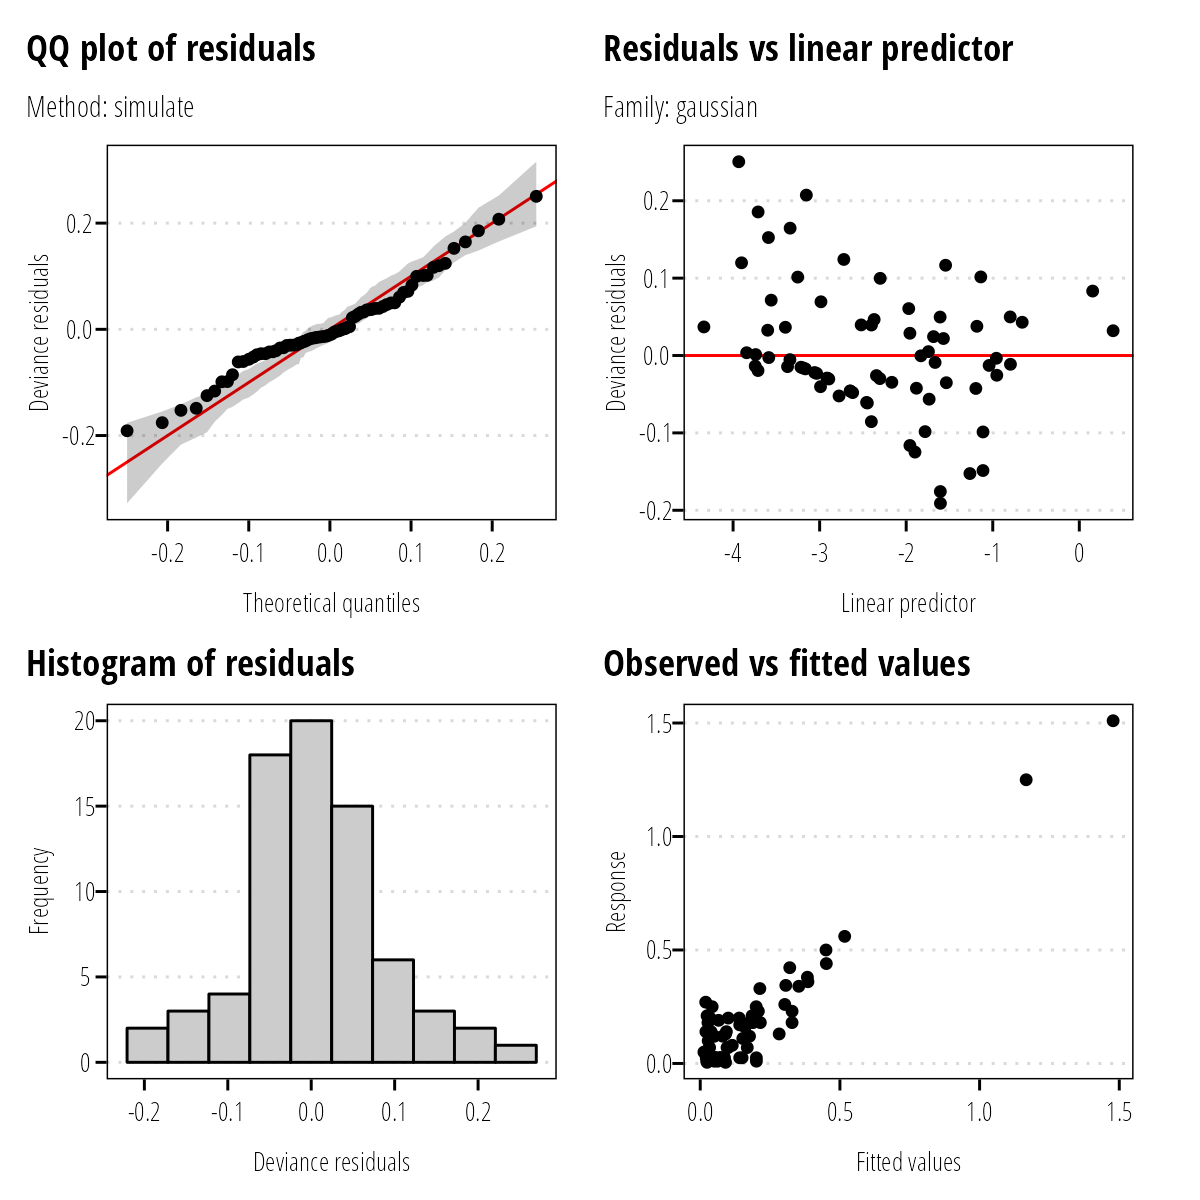
\includegraphics{model_assessment_files/figure-pdf/unnamed-chunk-4-1.png}

}

\caption{Diagnostic plot for NO\textsubscript{3}-N model at
USGS-08164000}

\end{figure}

\begin{figure}[h]

{\centering 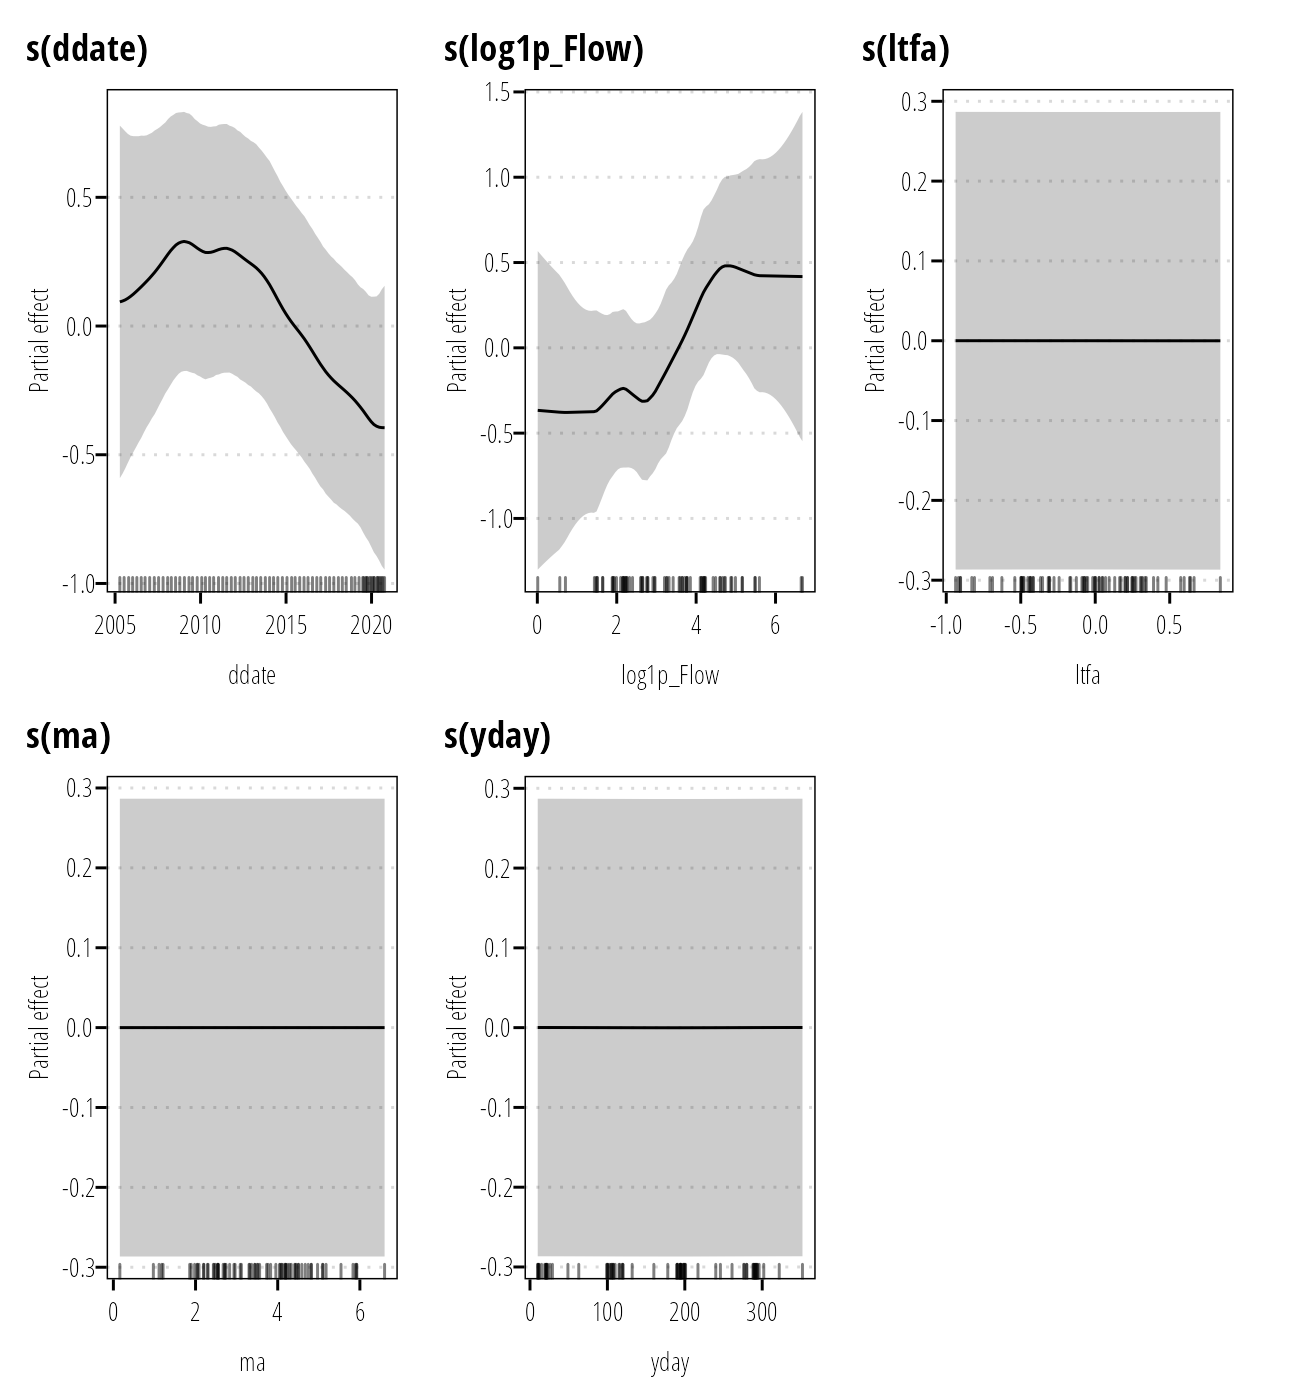
\includegraphics{model_assessment_files/figure-pdf/unnamed-chunk-5-1.png}

}

\caption{Partial effects of covariates in NO\textsubscript{3}-N model at
USGS-08164000}

\end{figure}

\begin{figure}[h]

{\centering 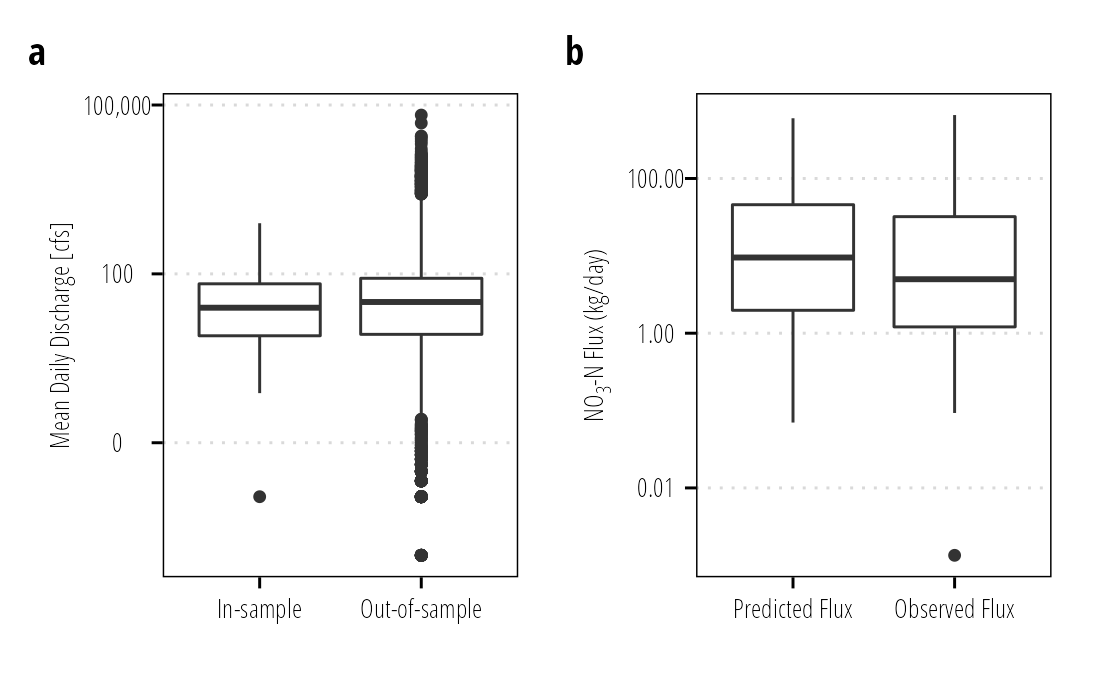
\includegraphics{model_assessment_files/figure-pdf/unnamed-chunk-6-1.png}

}

\caption{Comparisons of (a) in-sample and out-of-sample mean daily
discharge and (b) predicted daily fluxes (for both sampled and
non-sampled days) and measured daily fluxes.}

\end{figure}

\begin{figure}[h]

{\centering 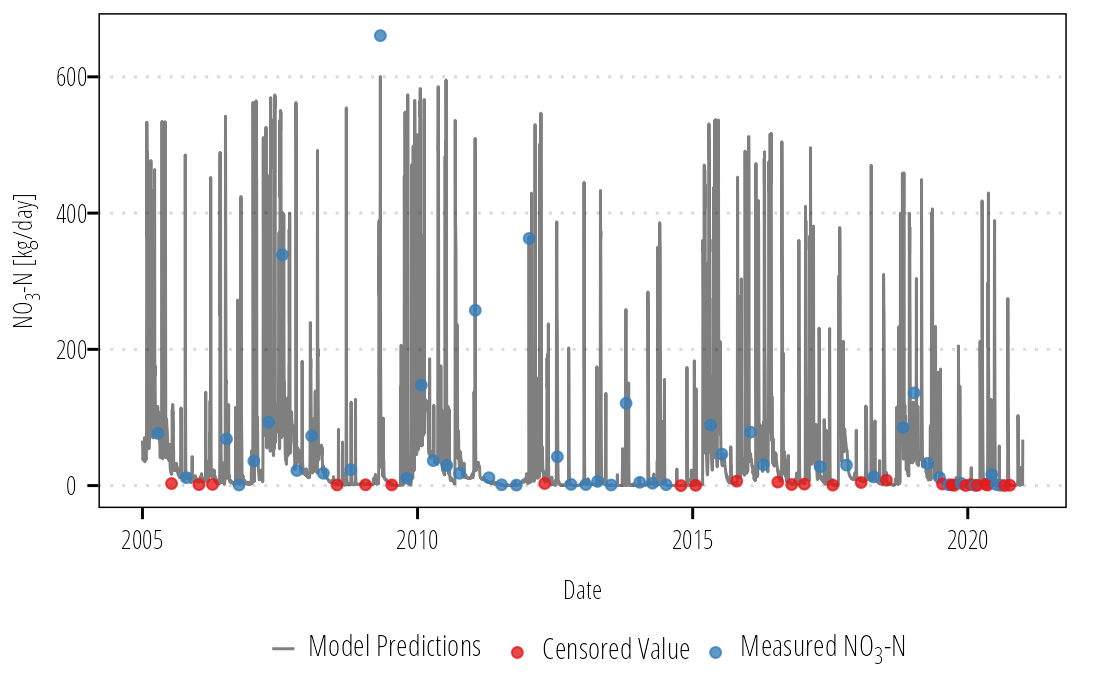
\includegraphics{model_assessment_files/figure-pdf/unnamed-chunk-7-1.png}

}

\caption{Time series plot of NO\textsubscript{3}-N model predictions and
observed values at USGS-08164000}

\end{figure}

\clearpage

\hypertarget{tp}{%
\subsubsection{TP}\label{tp}}

\begin{widestuff}

\caption{TP GAM summary - Lavaca River at Edna, USGS-08164000.}
\centering
\begin{tabular}[t]{llllllrll}
\toprule
Component & Term & Estimate & Std.Error & t-value & edf & ref.df & F-value & p-value\textsuperscript{1}\\
\midrule
A. parametric coefficients & (Intercept) & -1.611 & 0.045 & -35.811 &  &  &  & 0.000 ***\\
\cmidrule{1-9}
 & s(ddate) &  &  &  & 3.262 & 17 & 0.408 & 0.045 *\\

 & s(yday) &  &  &  & 1.266 & 8 & 0.352 & 0.094 +\\

 & s(log1p(Flow)) &  &  &  & 0.953 & 4 & 0.405 & 0.133\\

 & s(ma) &  &  &  & 0.000 & 5 & 0.000 & 0.510\\

\multirow[t]{-5}{*}{\raggedright\arraybackslash B. smooth terms} & s(stfa) &  &  &  & 2.585 & 4 & 2.857 & 0.003 **\\
\bottomrule
\multicolumn{9}{l}{\textsuperscript{1} Signif. codes: 0 <= '***' < 0.001 < '**' < 0.01 < '*' < 0.05 < '+' < 0.1}\\
\multicolumn{9}{l}{\textsuperscript{} Adjusted R-squared: 0.274, Deviance explained 0.250}\\
\multicolumn{9}{l}{\textsuperscript{} -REML : -70.944, Scale est: 0.162, N: 80}\\
\end{tabular}
\end{widestuff}

\hypertarget{tbl-TP308164000-CV}{}
\begin{longtable}[]{@{}lc@{}}
\caption{\label{tbl-TP308164000-CV}Summary of goodness-of-fit metrics
for 5-fold cross-validation of TP load GAM at Lavaca River at Edna,
USGS-08164000.}\tabularnewline
\toprule()
\textbf{Goodness of Fit Metric} & \textbf{Median (IQR)} \\
\midrule()
\endfirsthead
\toprule()
\textbf{Goodness of Fit Metric} & \textbf{Median (IQR)} \\
\midrule()
\endhead
KGE & 0.77 (0.71, 0.81) \\
R\textsuperscript{2} & 0.77 (0.72, 0.82) \\
Percent Bias & -7.45 (-9.10, -6.35) \\
\bottomrule()
\end{longtable}

\clearpage

\begin{figure}[h]

{\centering 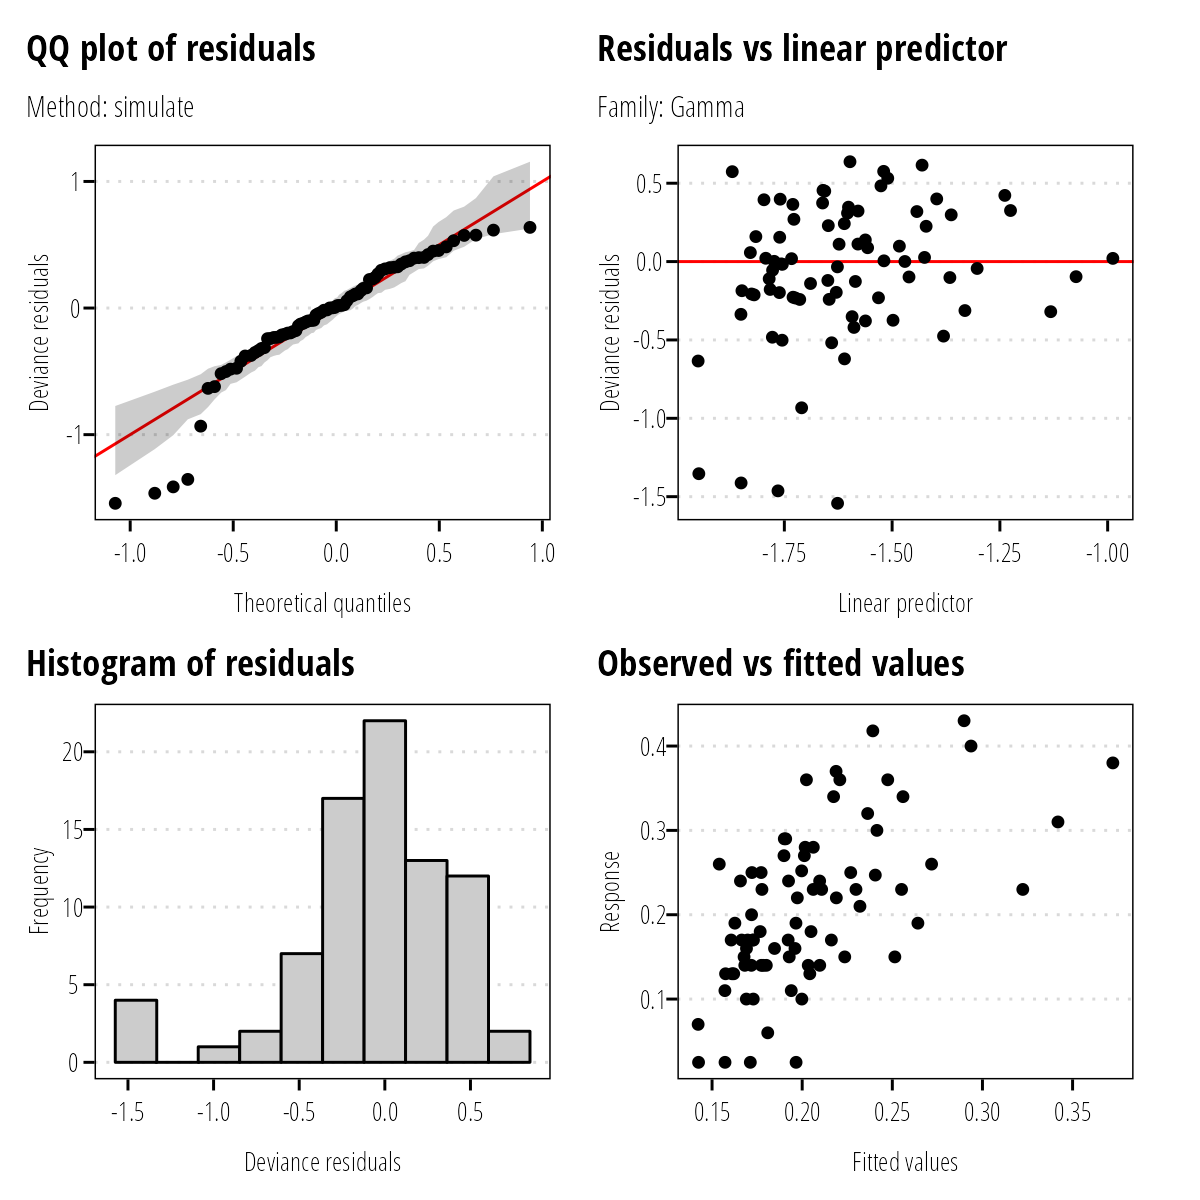
\includegraphics{model_assessment_files/figure-pdf/unnamed-chunk-10-1.png}

}

\caption{Diagnostic plot for TP model at USGS-08164000}

\end{figure}

\begin{figure}[h]

{\centering 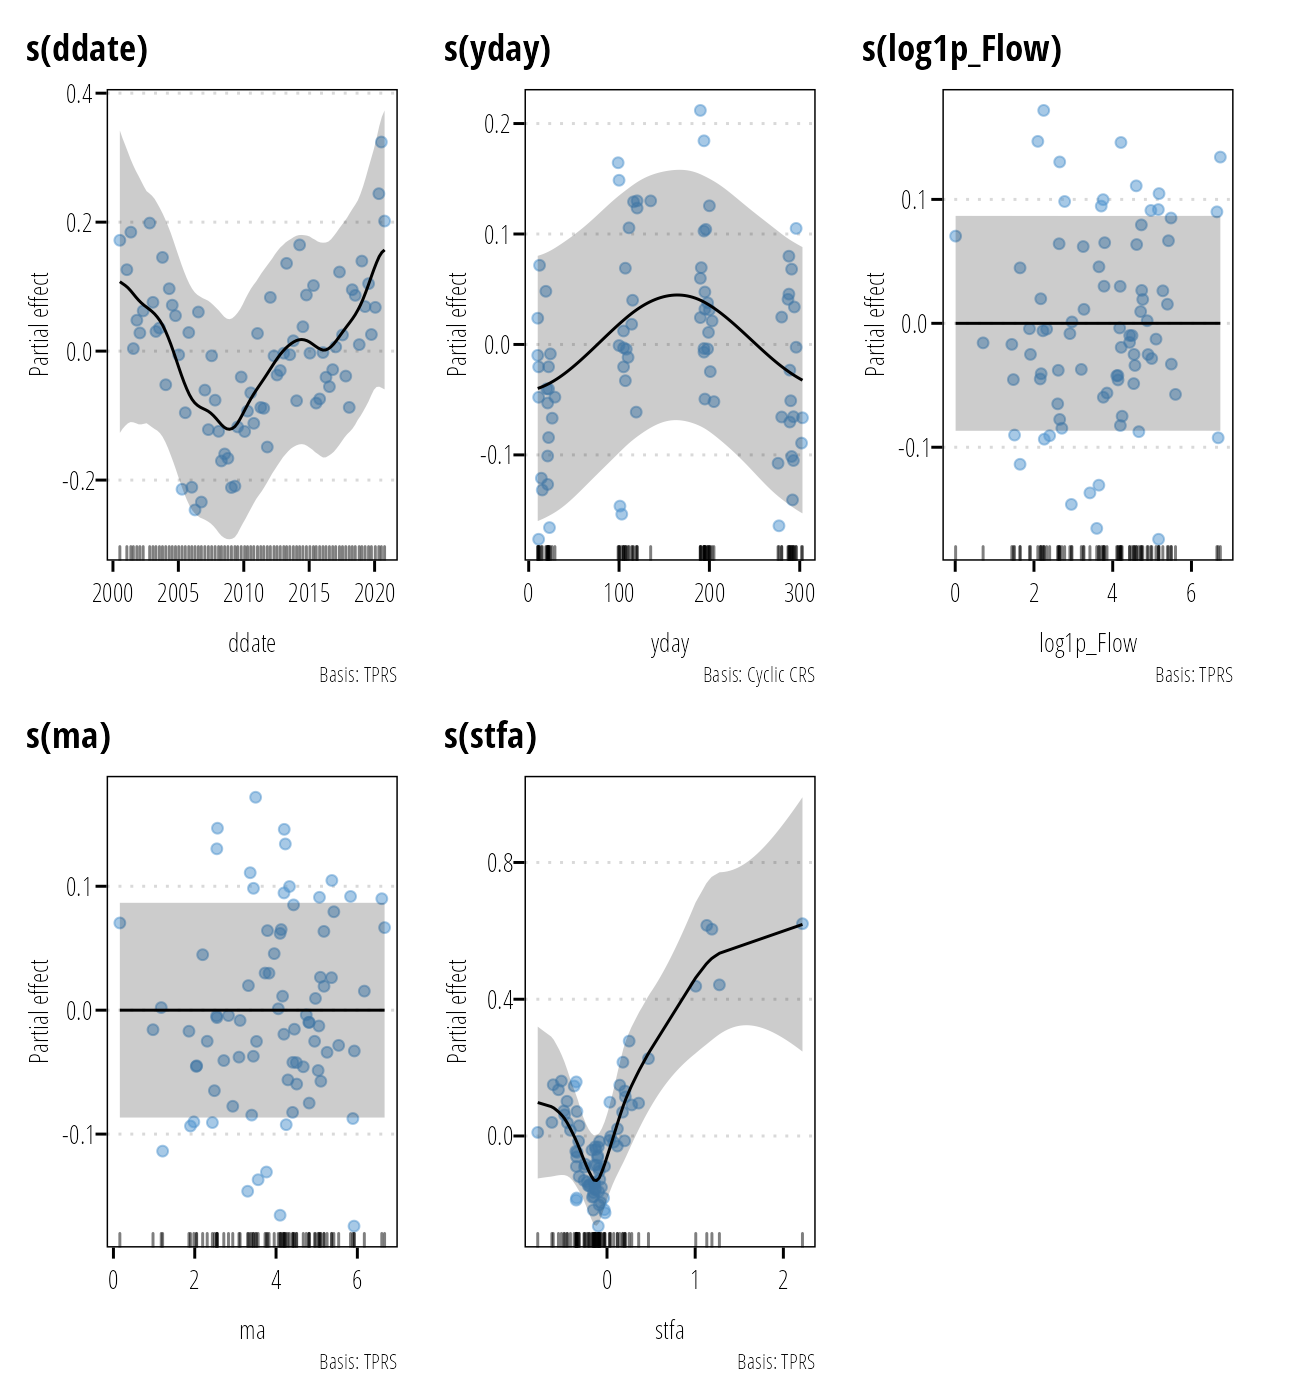
\includegraphics{model_assessment_files/figure-pdf/unnamed-chunk-11-1.png}

}

\caption{Partial effects of covariates in TP model at USGS-08164000}

\end{figure}

\begin{figure}[h]

{\centering 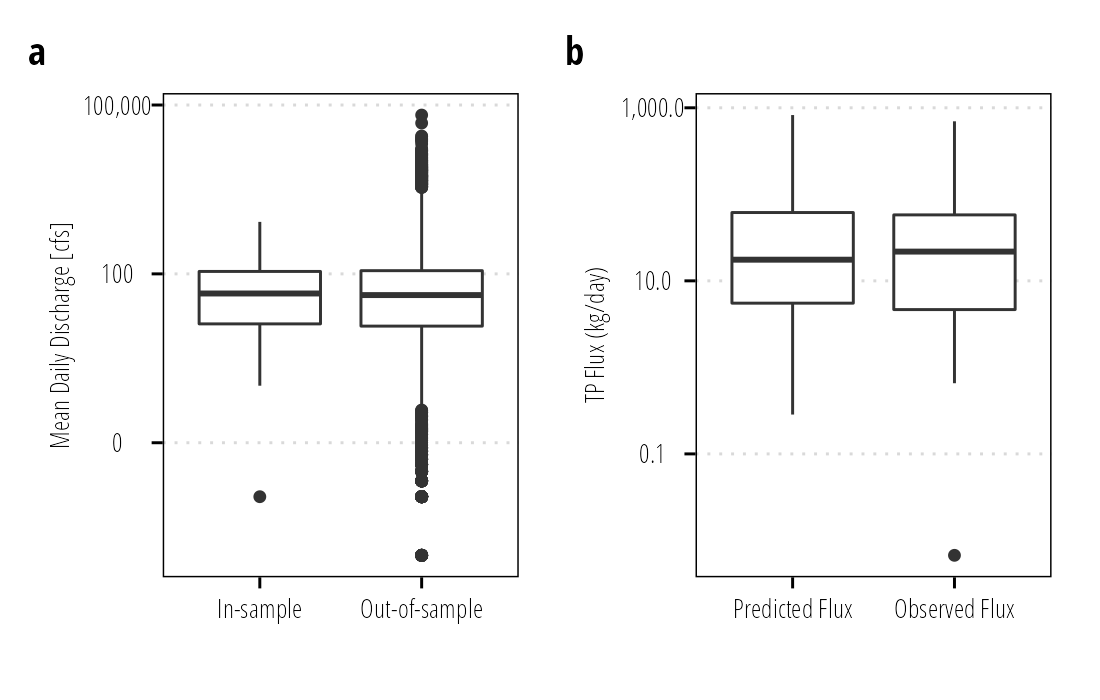
\includegraphics{model_assessment_files/figure-pdf/unnamed-chunk-12-1.png}

}

\caption{Comparisons of (a) in-sample and out-of-sample mean daily
discharge and (b) predicted daily fluxes (for both sampled and
non-sampled days) and measured daily fluxes.}

\end{figure}

\begin{figure}[h]

{\centering 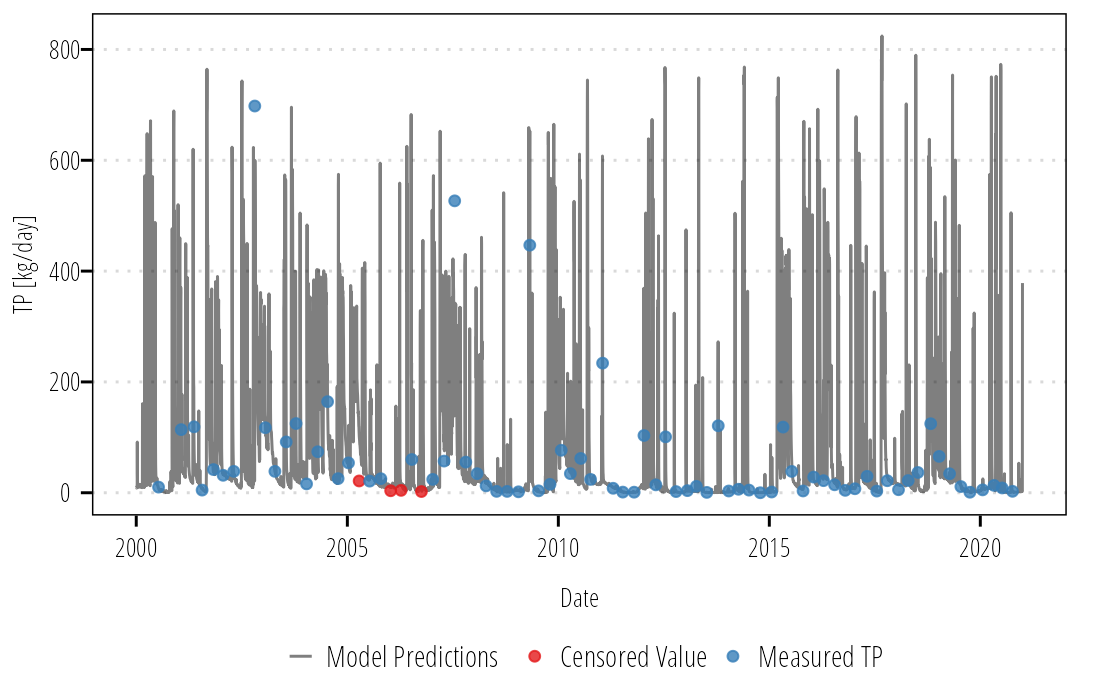
\includegraphics{model_assessment_files/figure-pdf/unnamed-chunk-13-1.png}

}

\caption{Time series plot of TP model predictions and observed values at
USGS-08164000}

\end{figure}

\clearpage

\hypertarget{navidad-river-at-strane-pk-nr-edna-08164390}{%
\subsection{Navidad River at Strane Pk nr Edna,
08164390}\label{navidad-river-at-strane-pk-nr-edna-08164390}}

\hypertarget{no3}{%
\subsubsection{\texorpdfstring{NO\textsubscript{3}}{NO3}}\label{no3}}

\begin{widestuff}

\caption{NO\textsubscript{3}-N GAM summary - Navidad River at Strane Pk nr Edna, USGS-08164390.}
\centering
\begin{tabular}[t]{llllllrll}
\toprule
Component & Term & Estimate & Std.Error & t-value & edf & ref.df & F-value & p-value\textsuperscript{1}\\
\midrule
A. parametric coefficients & (Intercept) & -2.010 & 0.100 & -20.154 &  &  &  & 0.000 ***\\
\cmidrule{1-9}
 & s(ddate) &  &  &  & 1.285 & 17 & 0.704 & 0.001 ***\\

 & s(yday) &  &  &  & 2.541 & 4 & 5.150 & 0.000 ***\\

 & s(log1p(Flow)) &  &  &  & 3.788 & 5 & 4.777 & 0.000 ***\\

 & s(stfa) &  &  &  & 2.992 & 5 & 3.209 & 0.001 ***\\

\multirow[t]{-5}{*}{\raggedright\arraybackslash B. smooth terms} & s(ma) &  &  &  & 0.000 & 4 & 0.000 & 0.308\\
\bottomrule
\multicolumn{9}{l}{\textsuperscript{1} Signif. codes: 0 <= '***' < 0.001 < '**' < 0.01 < '*' < 0.05 < '+' < 0.1}\\
\multicolumn{9}{l}{\textsuperscript{} Adjusted R-squared: 0.720, Deviance explained 0.770}\\
\multicolumn{9}{l}{\textsuperscript{} -REML : -46.798, Scale est: 0.00726, N: 59}\\
\end{tabular}
\end{widestuff}

\hypertarget{tbl-NO308164390-CV}{}
\begin{longtable}[]{@{}lc@{}}
\caption{\label{tbl-NO308164390-CV}Summary of goodness-of-fit metrics
for 5-fold cross-validation of NO\textsubscript{3}-N concentration GAM
at Navidad River at Strane Pk nr Edna,,
USGS-NO308164390.}\tabularnewline
\toprule()
\textbf{Goodness of Fit Metric} & \textbf{Median (IQR)} \\
\midrule()
\endfirsthead
\toprule()
\textbf{Goodness of Fit Metric} & \textbf{Median (IQR)} \\
\midrule()
\endhead
KGE & 0.60 (0.58, 0.65) \\
R\textsuperscript{2} & 0.71 (0.65, 0.77) \\
Percent Bias & -18.4 (-21.4, -16.5) \\
\bottomrule()
\end{longtable}

\clearpage

\begin{figure}[h]

{\centering 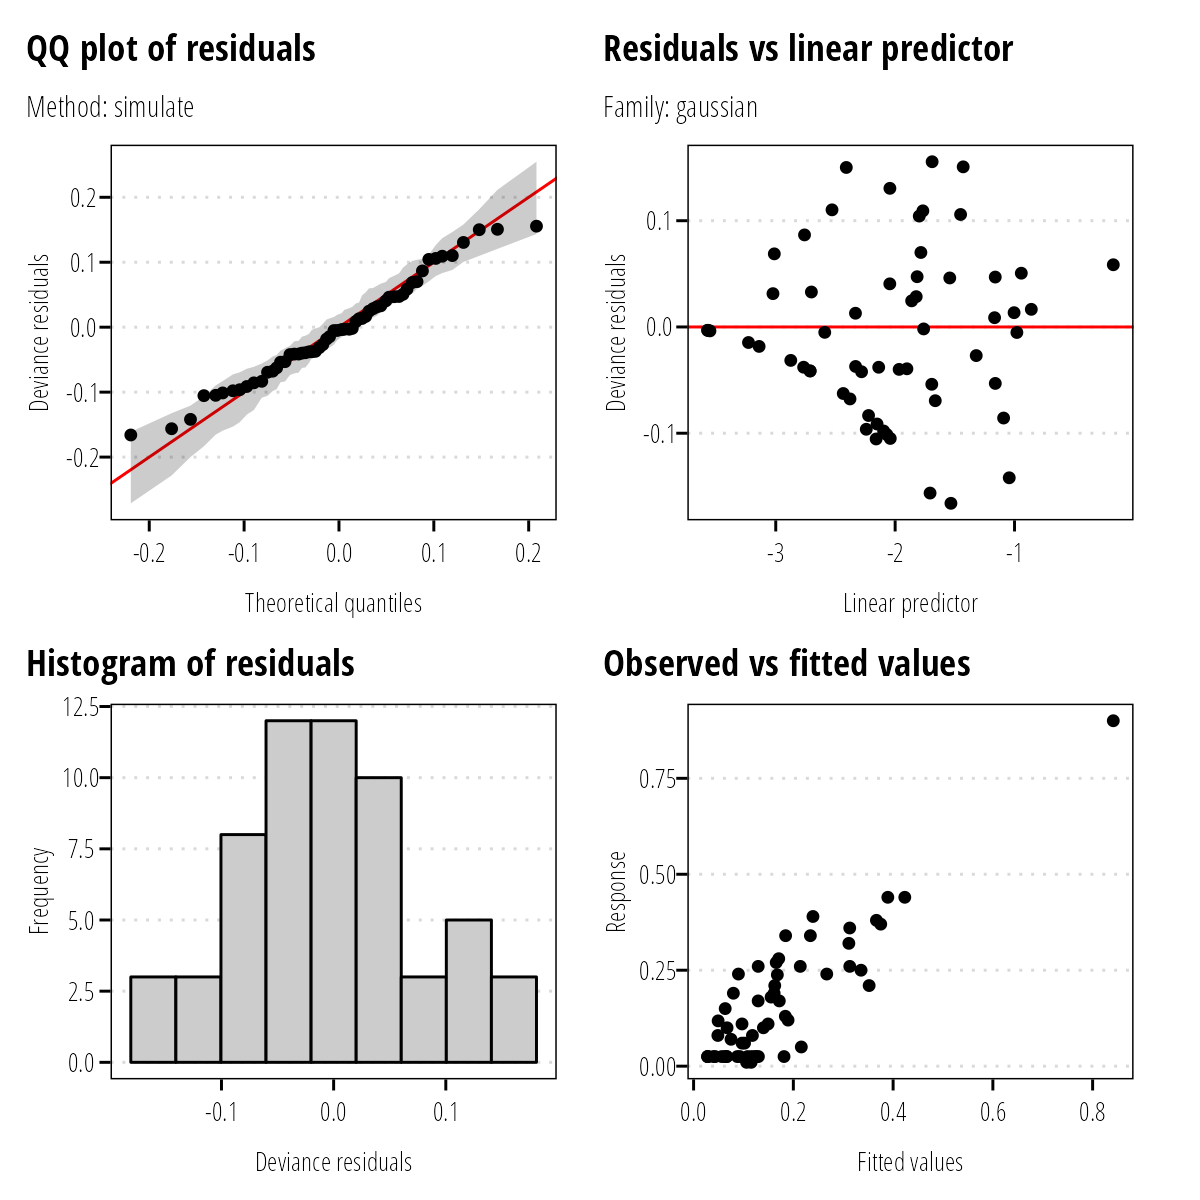
\includegraphics{model_assessment_files/figure-pdf/unnamed-chunk-16-1.png}

}

\caption{Diagnostic plot for NO\textsubscript{3} model at
USGS-08164390.}

\end{figure}

\begin{figure}[h]

{\centering 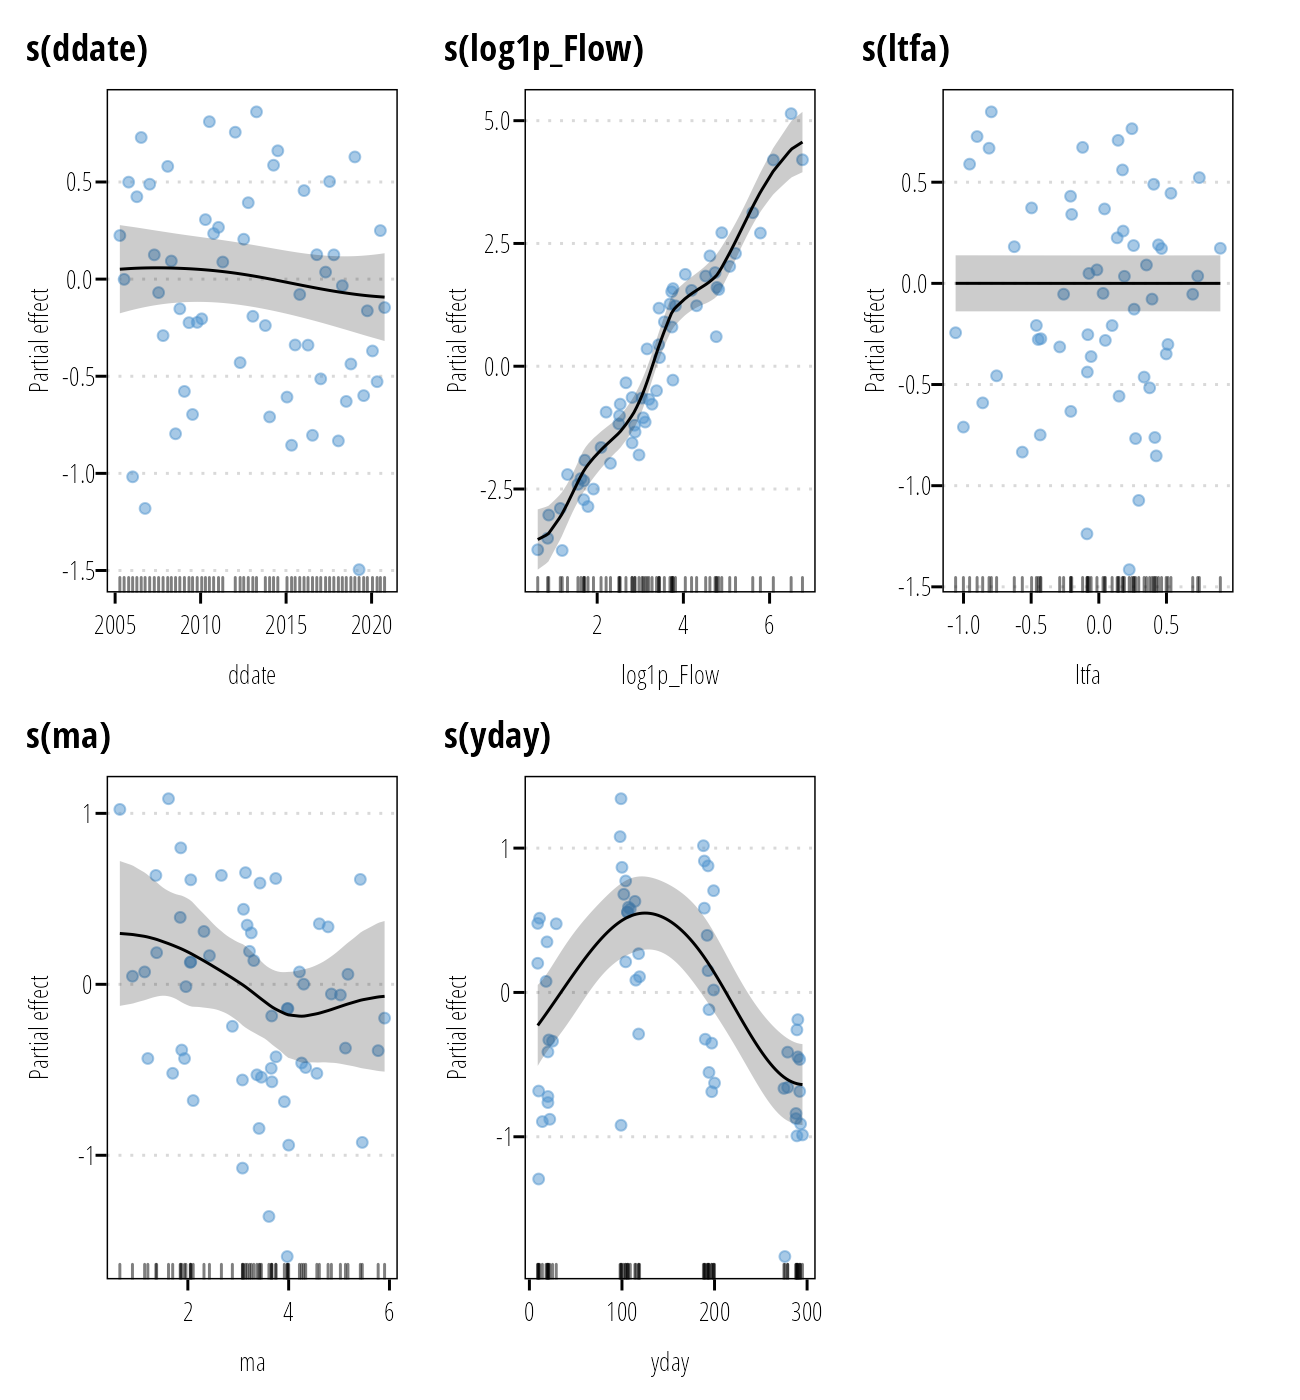
\includegraphics{model_assessment_files/figure-pdf/unnamed-chunk-17-1.png}

}

\caption{Partial effects of covariates in NO\textsubscript{3}-N model at
USGS-08164390.}

\end{figure}

\begin{figure}[h]

{\centering 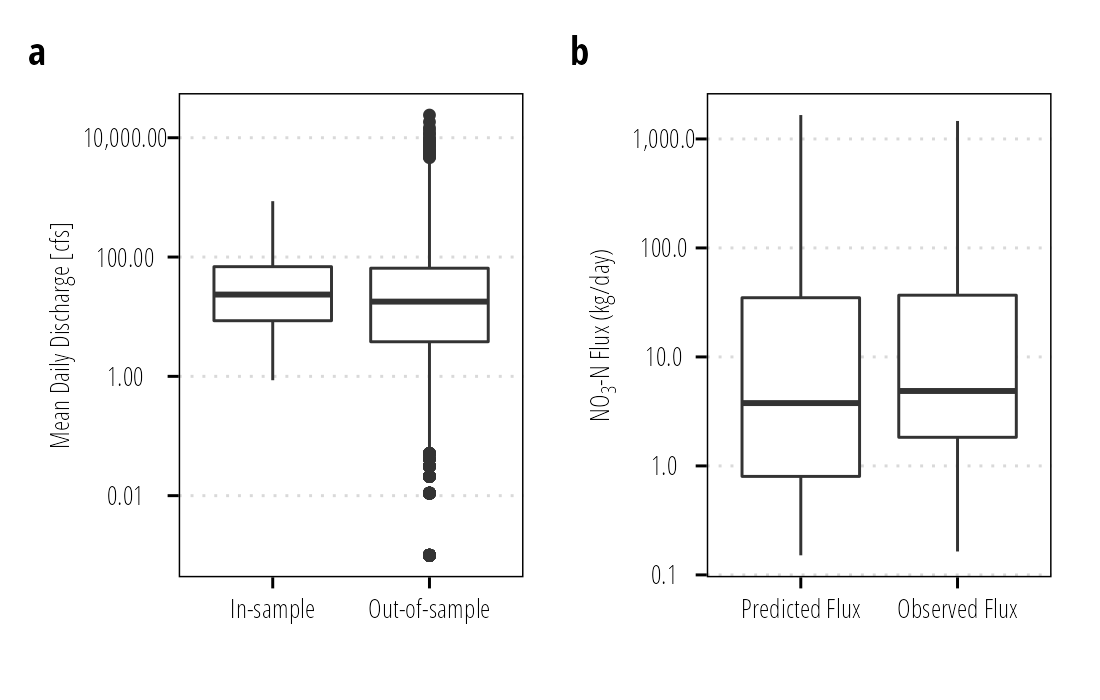
\includegraphics{model_assessment_files/figure-pdf/unnamed-chunk-18-1.png}

}

\caption{Comparisons of (a) in-sample and out-of-sample mean daily
discharge and (b) predicted daily fluxes (for both sampled and
non-sampled days) and measured daily fluxes.}

\end{figure}

\begin{figure}[h]

{\centering 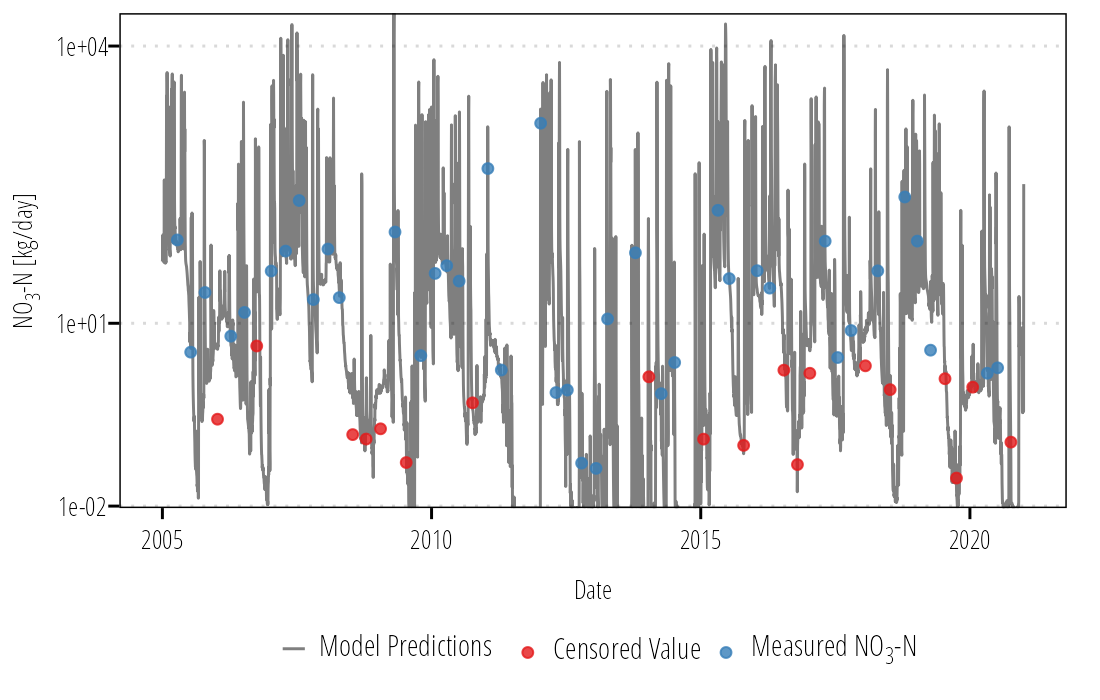
\includegraphics{model_assessment_files/figure-pdf/unnamed-chunk-19-1.png}

}

\caption{Time series plot of NO\textsubscript{3} model predictions and
observed values at USGS-08164390.}

\end{figure}

\clearpage

\hypertarget{tp-1}{%
\subsubsection{TP}\label{tp-1}}

\begin{widestuff}

\caption{TP GAM summary - Navidad River at Strane Pk nr Edna, USGS-08164390.}
\centering
\begin{tabular}[t]{llllllrll}
\toprule
Component & Term & Estimate & Std.Error & t-value & edf & ref.df & F-value & p-value\textsuperscript{1}\\
\midrule
A. parametric coefficients & (Intercept) & -1.597 & 0.038 & -42.298 &  &  &  & 0.000 ***\\
\cmidrule{1-9}
 & s(ddate) &  &  &  & 7.120 & 17 & 3.465 & 0.000 ***\\

 & s(yday) &  &  &  & 0.456 & 4 & 0.147 & 0.270\\

 & s(log1p(Flow)) &  &  &  & 2.630 & 5 & 2.428 & 0.002 **\\

 & s(stfa) &  &  &  & 0.000 & 5 & 0.000 & 0.690\\

\multirow[t]{-5}{*}{\raggedright\arraybackslash B. smooth terms} & s(ma) &  &  &  & 0.000 & 5 & 0.000 & 0.759\\
\bottomrule
\multicolumn{9}{l}{\textsuperscript{1} Signif. codes: 0 <= '***' < 0.001 < '**' < 0.01 < '*' < 0.05 < '+' < 0.1}\\
\multicolumn{9}{l}{\textsuperscript{} Adjusted R-squared: 0.550, Deviance explained 0.486}\\
\multicolumn{9}{l}{\textsuperscript{} -REML : -76.491, Scale est: 0.110, N: 77}\\
\end{tabular}
\end{widestuff}

\hypertarget{tbl-TP08164390-CV}{}
\begin{longtable}[]{@{}lc@{}}
\caption{\label{tbl-TP08164390-CV}Summary of goodness-of-fit metrics for
5-fold cross-validation of TP load GAM at Navidad River at Strane Pk nr
Edna, USGS-08164390.}\tabularnewline
\toprule()
\textbf{Goodness of Fit Metric} & \textbf{Median (IQR)} \\
\midrule()
\endfirsthead
\toprule()
\textbf{Goodness of Fit Metric} & \textbf{Median (IQR)} \\
\midrule()
\endhead
KGE & 0.951 (0.944, 0.960) \\
R\textsuperscript{2} & 0.982 (0.973, 0.984) \\
Percent Bias & -9.10 (-10.10, -8.27) \\
\bottomrule()
\end{longtable}

\clearpage

\begin{figure}[h]

{\centering 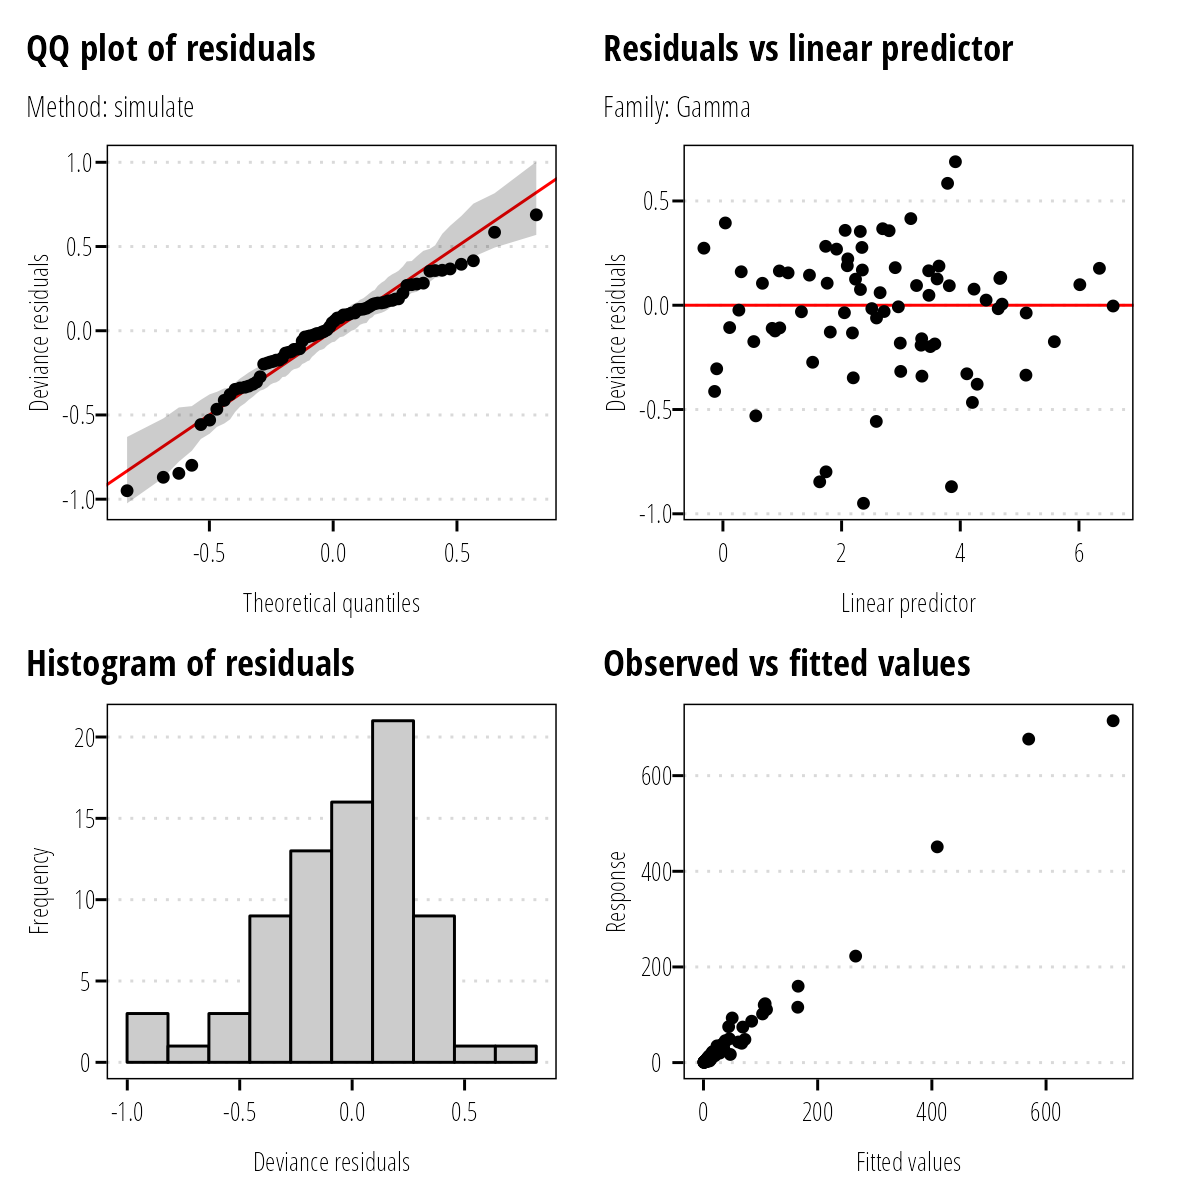
\includegraphics{model_assessment_files/figure-pdf/unnamed-chunk-22-1.png}

}

\caption{Diagnostic plot for TP model at USGS-08164390.}

\end{figure}

\begin{figure}[h]

{\centering 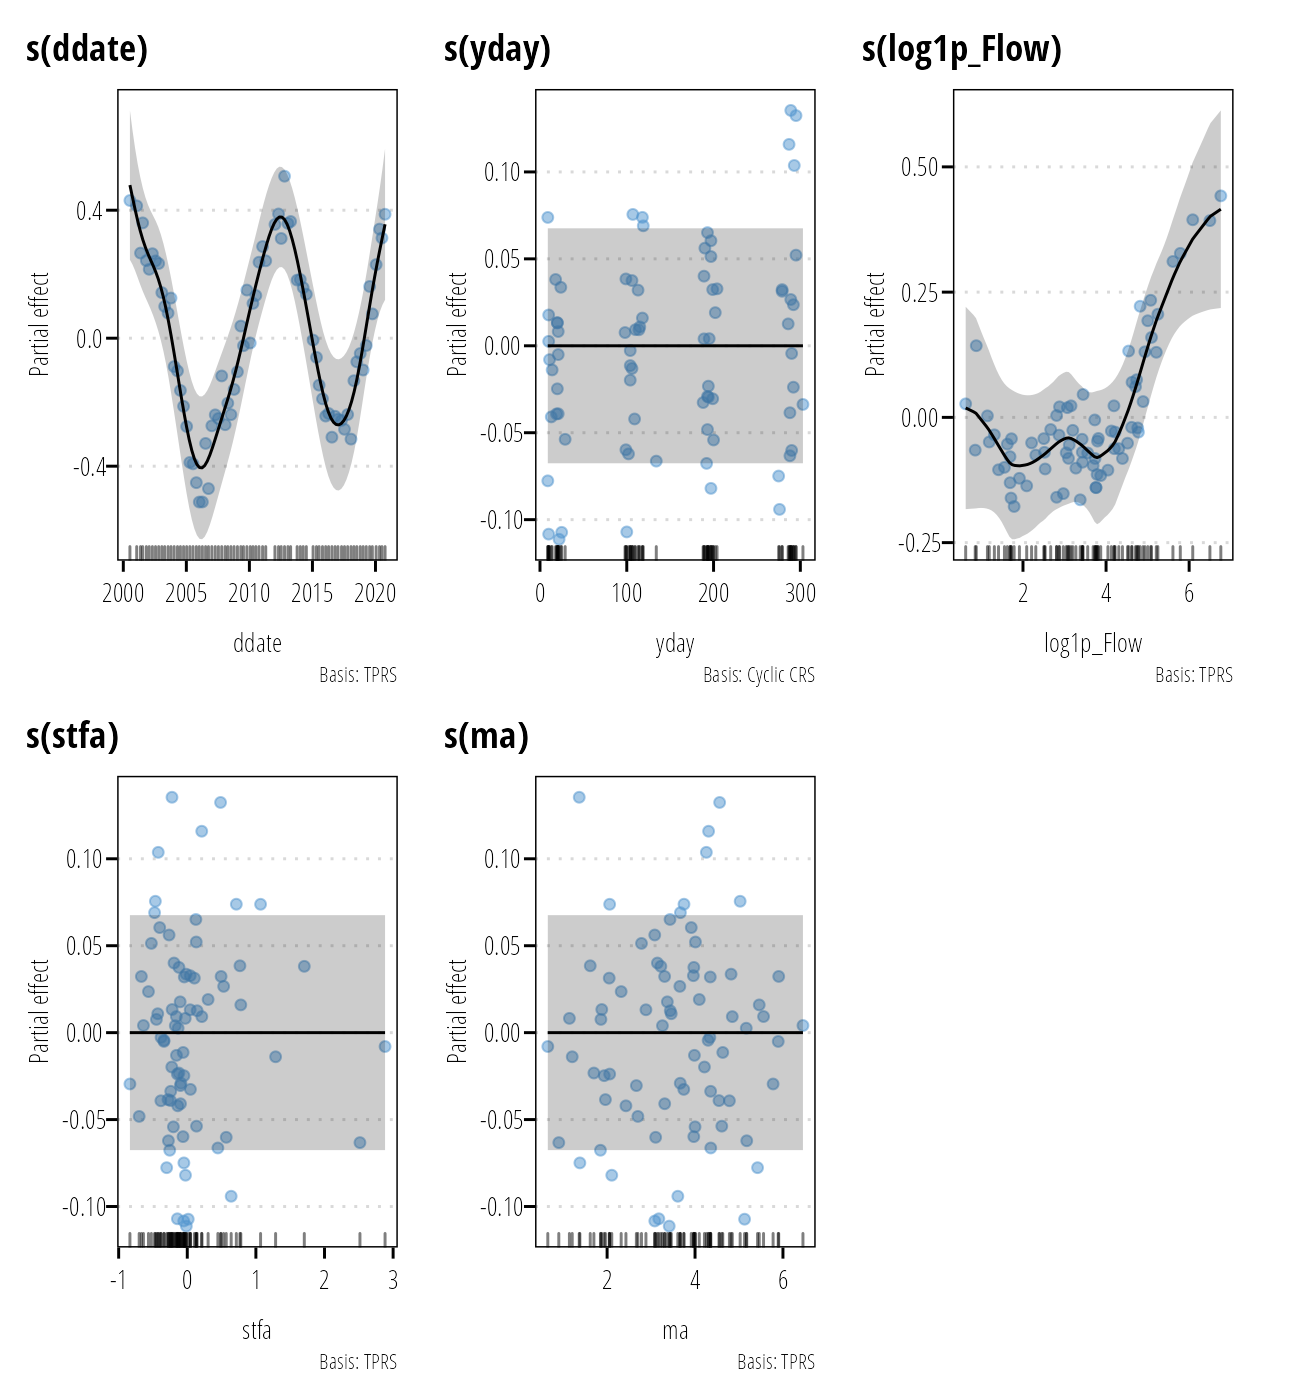
\includegraphics{model_assessment_files/figure-pdf/unnamed-chunk-23-1.png}

}

\caption{Partial effects of covariates in TP model at USGS-08164390.}

\end{figure}

\begin{figure}[h]

{\centering 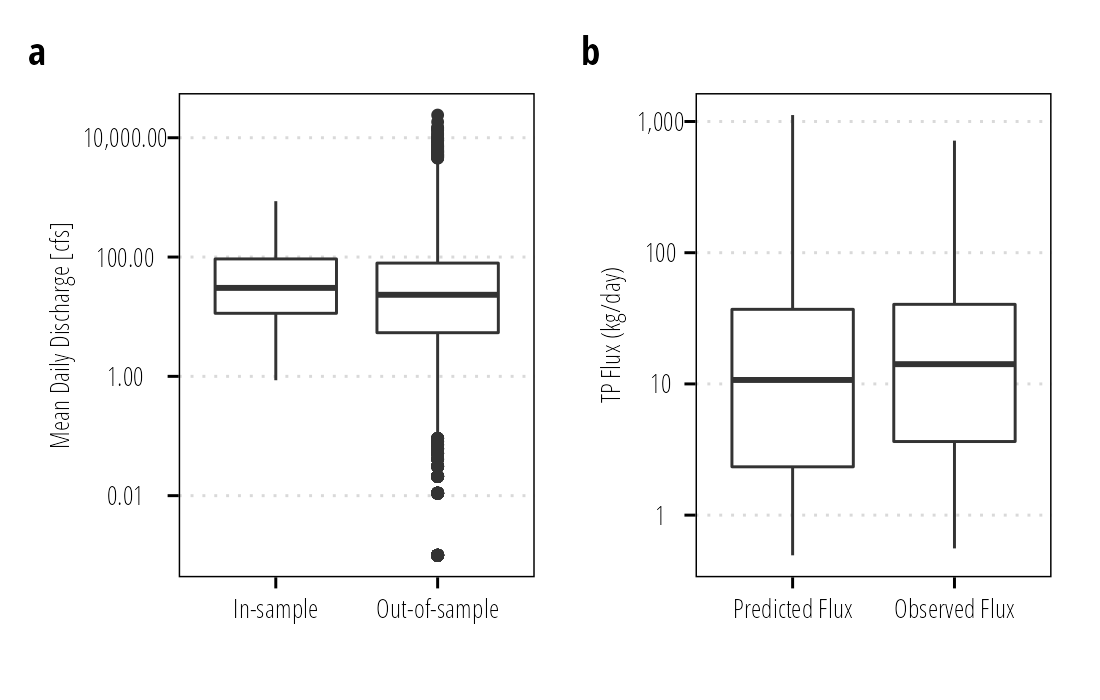
\includegraphics{model_assessment_files/figure-pdf/unnamed-chunk-24-1.png}

}

\caption{Comparisons of (a) in-sample and out-of-sample mean daily
discharge and (b) predicted daily fluxes (for both sampled and
non-sampled days) and measured daily fluxes.}

\end{figure}

\begin{figure}[h]

{\centering 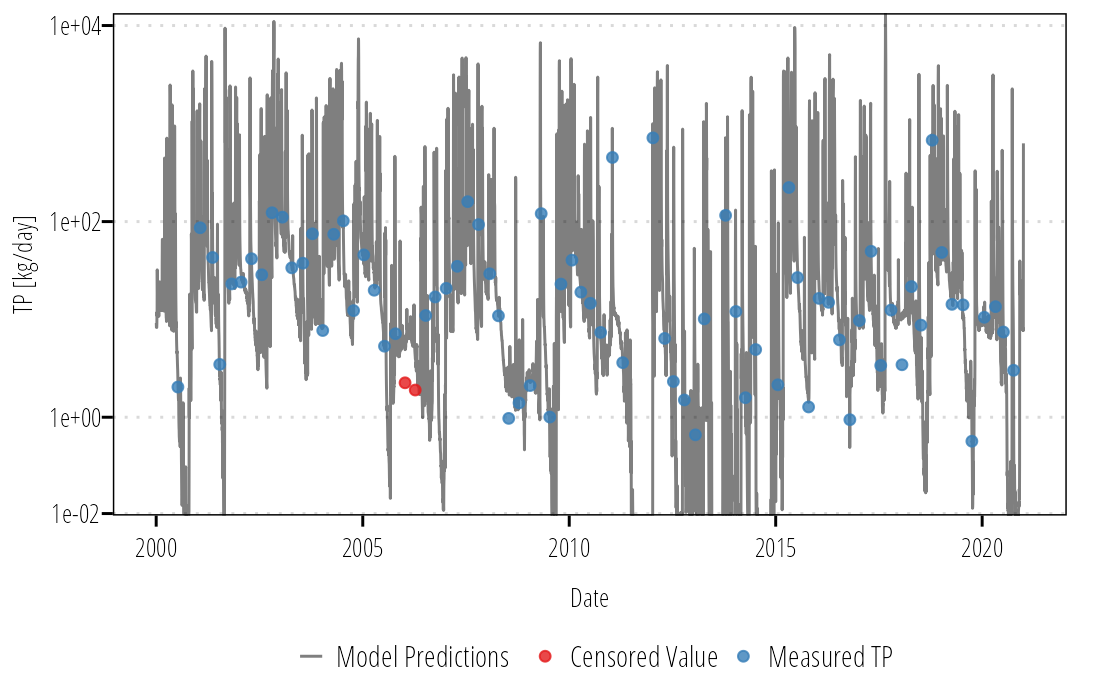
\includegraphics{model_assessment_files/figure-pdf/unnamed-chunk-25-1.png}

}

\caption{Time series plot of TP model predictions and observed values at
USGS-08164390.}

\end{figure}

\clearpage

\hypertarget{sandy-creek-nr-ganado-usgs-08164450}{%
\subsection{Sandy Creek nr Ganado,
USGS-08164450}\label{sandy-creek-nr-ganado-usgs-08164450}}

\hypertarget{no3-1}{%
\subsubsection{\texorpdfstring{NO\textsubscript{3}}{NO3}}\label{no3-1}}

\begin{widestuff}

\caption{NO\textsubscript{3}-N GAM summary - Sandy Creek nr Ganado, USGS-08164450.}
\centering
\begin{tabular}[t]{llllllrll}
\toprule
Component & Term & Estimate & Std.Error & t-value & edf & ref.df & F-value & p-value\textsuperscript{1}\\
\midrule
A. parametric coefficients & (Intercept) & -1.942 & 0.081 & -24.046 &  &  &  & 0.000 ***\\
\cmidrule{1-9}
 & s(ddate) &  &  &  & 0.000 & 17 & 0.000 & 0.916\\

 & s(yday) &  &  &  & 2.018 & 4 & 2.777 & 0.003 **\\

 & s(log1p(Flow)) &  &  &  & 2.338 & 9 & 0.481 & 0.101\\

 & s(stfa) &  &  &  & 0.000 & 5 & 0.000 & 0.585\\

\multirow[t]{-5}{*}{\raggedright\arraybackslash B. smooth terms} & s(ma) &  &  &  & 4.201 & 5 & 5.113 & 0.000 ***\\
\bottomrule
\multicolumn{9}{l}{\textsuperscript{1} Signif. codes: 0 <= '***' < 0.001 < '**' < 0.01 < '*' < 0.05 < '+' < 0.1}\\
\multicolumn{9}{l}{\textsuperscript{} Adjusted R-squared: 0.261, Deviance explained 0.505}\\
\multicolumn{9}{l}{\textsuperscript{} -REML : -51.428, Scale est: 0.365, N: 56}\\
\end{tabular}
\end{widestuff}

\hypertarget{tbl-NO308164450-CV}{}
\begin{longtable}[]{@{}lc@{}}
\caption{\label{tbl-NO308164450-CV}Summary of goodness-of-fit metrics
for 5-fold cross-validation of NO\textsubscript{3}-N concentration GAM
at Sandy Creek nr Ganado, USGS-08164450.}\tabularnewline
\toprule()
\textbf{Goodness of Fit Metric} & \textbf{Median (IQR)} \\
\midrule()
\endfirsthead
\toprule()
\textbf{Goodness of Fit Metric} & \textbf{Median (IQR)} \\
\midrule()
\endhead
KGE & 0.47 (0.34, 0.50) \\
R\textsuperscript{2} & 0.49 (0.38, 0.57) \\
Percent Bias & -15 (-20, -8) \\
\bottomrule()
\end{longtable}

\clearpage

\begin{figure}[h]

{\centering 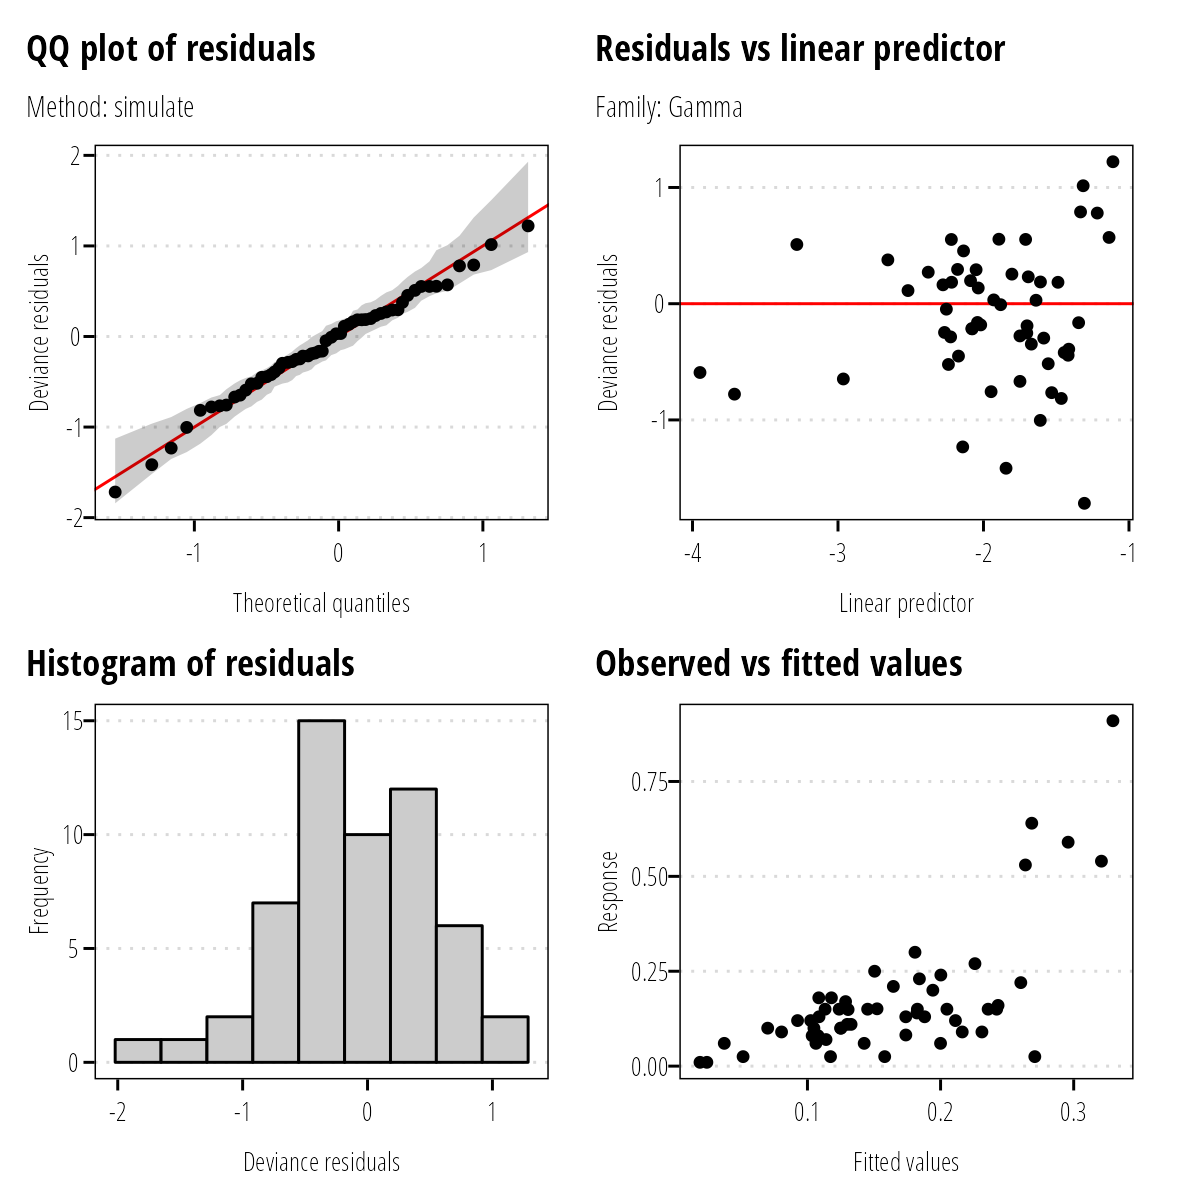
\includegraphics{model_assessment_files/figure-pdf/unnamed-chunk-28-1.png}

}

\caption{Diagnostic plot for NO\textsubscript{3} model at
USGS-08164450.}

\end{figure}

\begin{figure}[h]

{\centering 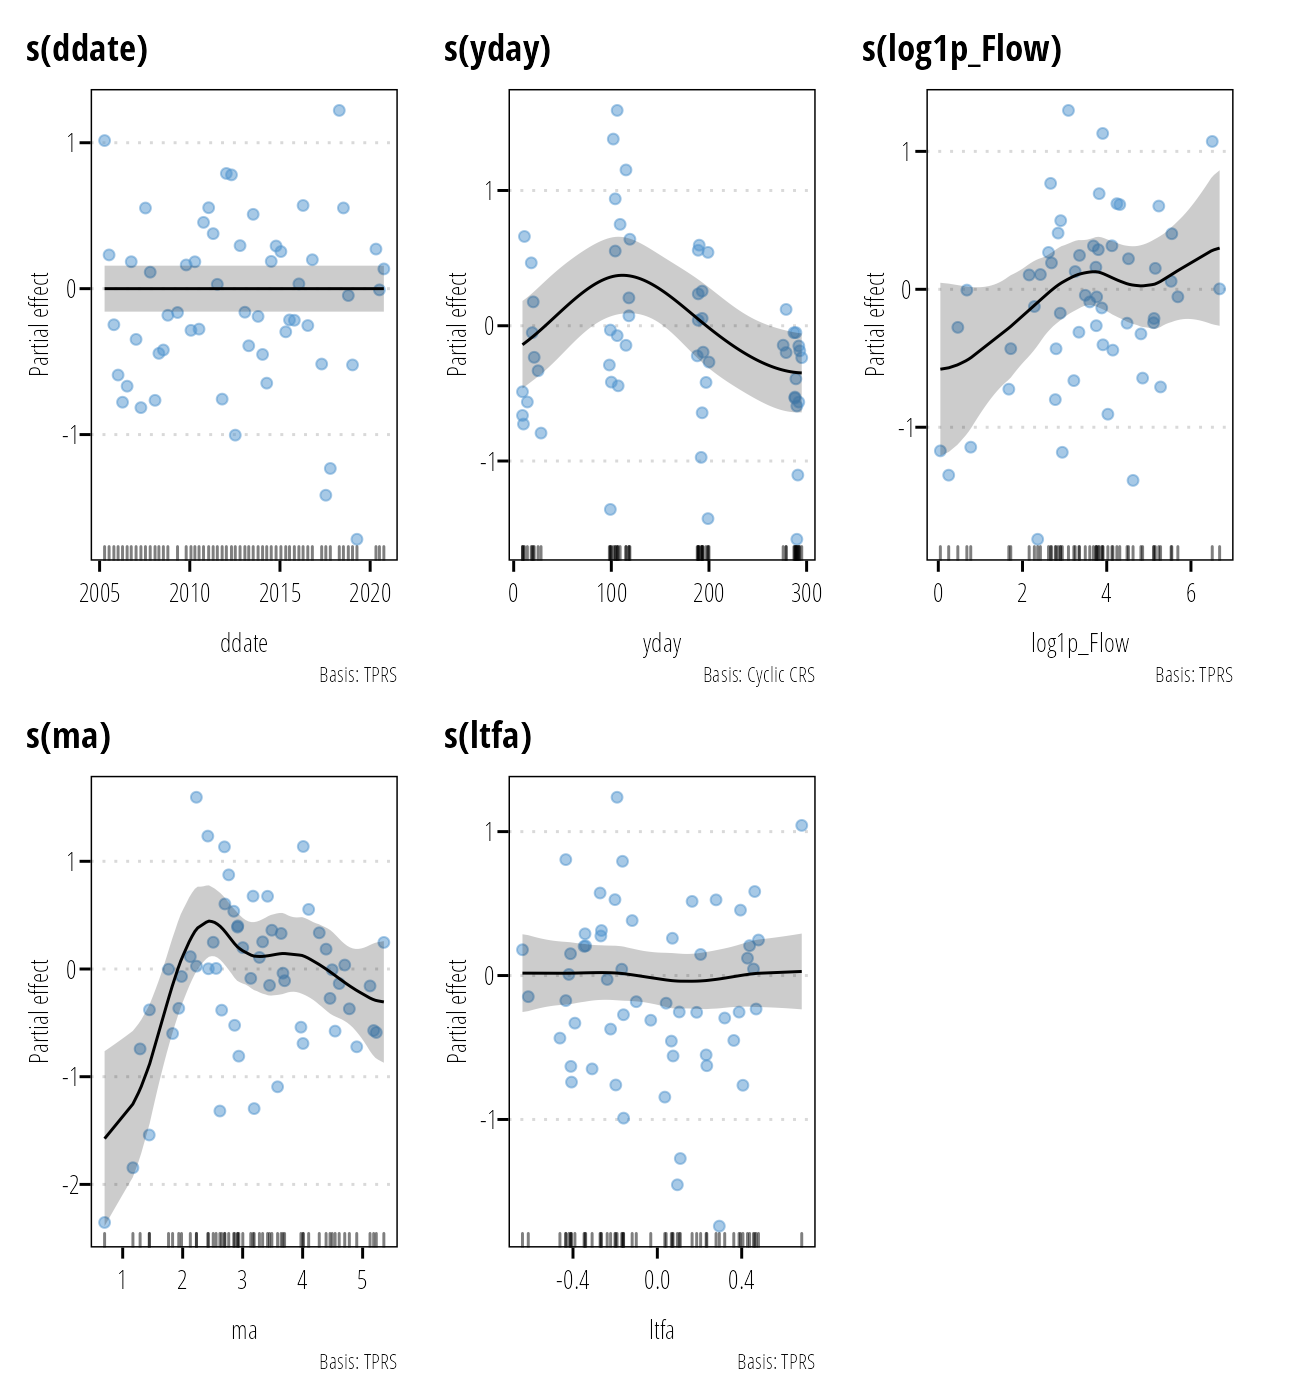
\includegraphics{model_assessment_files/figure-pdf/unnamed-chunk-29-1.png}

}

\caption{Partial effects of covariates in NO\textsubscript{3}-N model at
USGS-08164450.}

\end{figure}

\begin{figure}[h]

{\centering 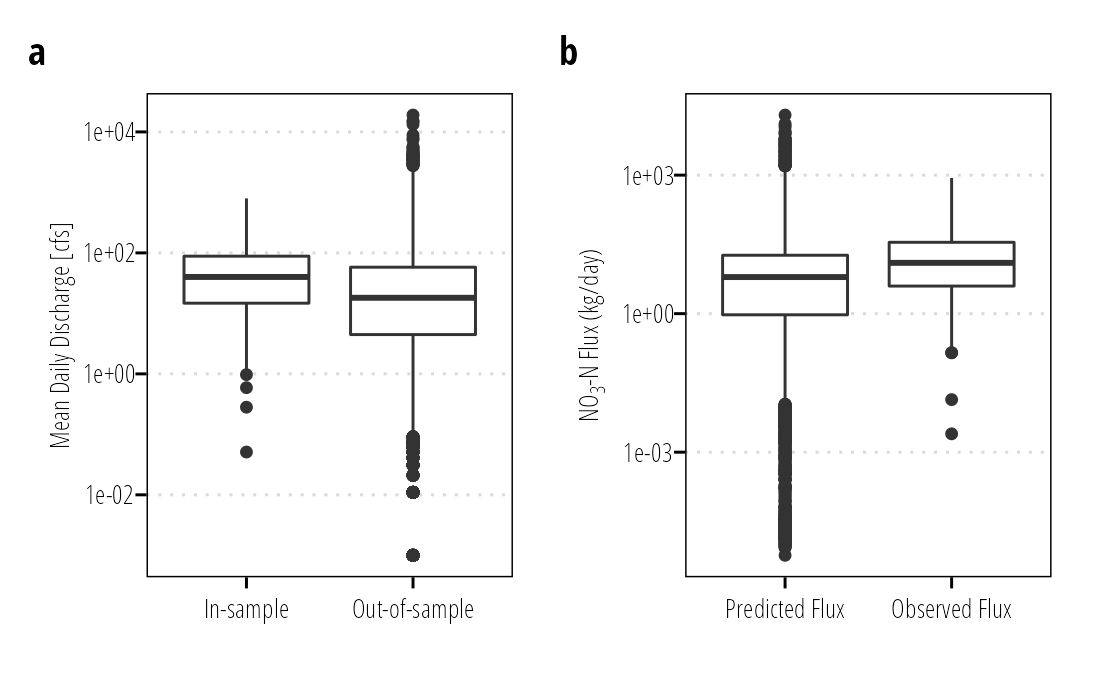
\includegraphics{model_assessment_files/figure-pdf/unnamed-chunk-30-1.png}

}

\caption{Comparisons of (a) in-sample and out-of-sample mean daily
discharge and (b) predicted daily fluxes (for both sampled and
non-sampled days) and measured daily fluxes.}

\end{figure}

\begin{figure}[h]

{\centering 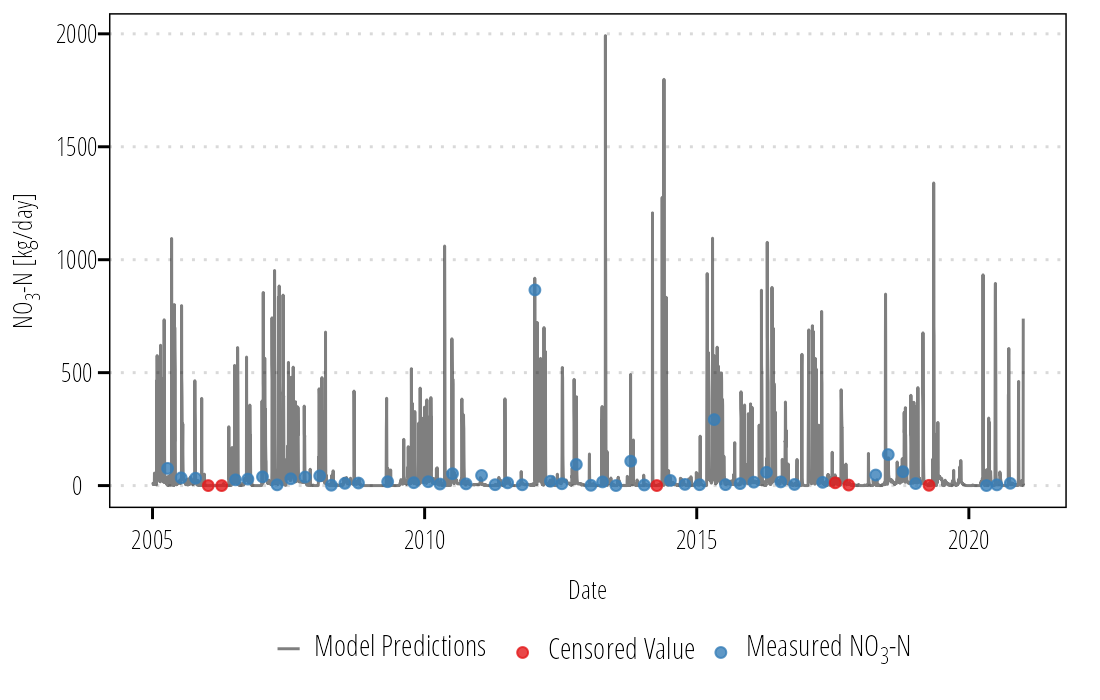
\includegraphics{model_assessment_files/figure-pdf/unnamed-chunk-31-1.png}

}

\caption{Time series plot of NO\textsubscript{3} model predictions and
observed values at USGS-08164450.}

\end{figure}

\clearpage

\hypertarget{tp-2}{%
\subsubsection{TP}\label{tp-2}}

\begin{widestuff}

\caption{TP GAM summary - Sandy Creek nr Ganado, USGS-08164450.}
\centering
\begin{tabular}[t]{llllllrll}
\toprule
Component & Term & Estimate & Std.Error & t-value & edf & ref.df & F-value & p-value\textsuperscript{1}\\
\midrule
A. parametric coefficients & (Intercept) & -1.729 & 0.067 & -25.973 &  &  &  & 0.000 ***\\
\cmidrule{1-9}
 & s(ddate) &  &  &  & 9.316 & 17 & 4.295 & 0.000 ***\\

 & s(yday) &  &  &  & 0.000 & 4 & 0.000 & 0.730\\

 & s(log1p(Flow)) &  &  &  & 6.939 & 9 & 2.967 & 0.000 ***\\

 & s(stfa) &  &  &  & 2.097 & 5 & 0.757 & 0.090 +\\

\multirow[t]{-5}{*}{\raggedright\arraybackslash B. smooth terms} & s(ma) &  &  &  & 2.171 & 4 & 3.529 & 0.000 ***\\
\bottomrule
\multicolumn{9}{l}{\textsuperscript{1} Signif. codes: 0 <= '***' < 0.001 < '**' < 0.01 < '*' < 0.05 < '+' < 0.1}\\
\multicolumn{9}{l}{\textsuperscript{} Adjusted R-squared: 0.757, Deviance explained 0.824}\\
\multicolumn{9}{l}{\textsuperscript{} -REML : -34.024, Scale est: 0.00944, N: 75}\\
\end{tabular}
\end{widestuff}

\hypertarget{tbl-TP08164450-CV}{}
\begin{longtable}[]{@{}lc@{}}
\caption{\label{tbl-TP08164450-CV}Summary of goodness-of-fit metrics for
5-fold cross-validation of TP load GAM at Sandy Creek nr Ganado,
USGS-08164450.}\tabularnewline
\toprule()
\textbf{Goodness of Fit Metric} & \textbf{Median (IQR)} \\
\midrule()
\endfirsthead
\toprule()
\textbf{Goodness of Fit Metric} & \textbf{Median (IQR)} \\
\midrule()
\endhead
KGE & 0.78 (0.56, 0.81) \\
R\textsuperscript{2} & 0.81 (0.67, 0.86) \\
Percent Bias & -6 (-9, -3) \\
\bottomrule()
\end{longtable}

\clearpage

\begin{figure}[h]

{\centering 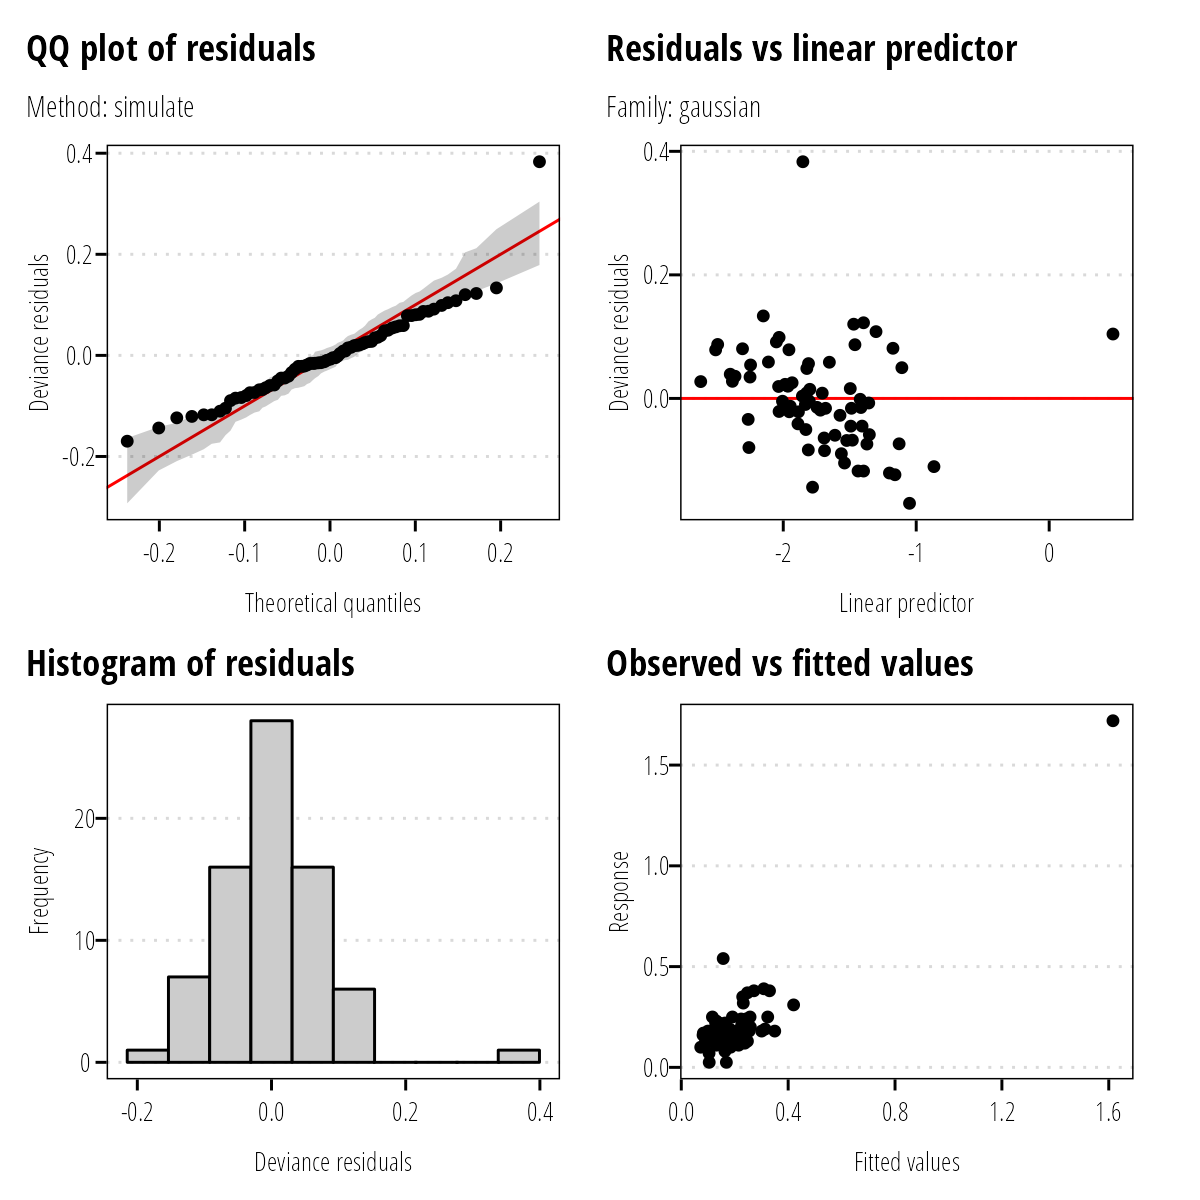
\includegraphics{model_assessment_files/figure-pdf/unnamed-chunk-34-1.png}

}

\caption{Diagnostic plot for TP model at USGS-08164450.}

\end{figure}

\begin{figure}[h]

{\centering 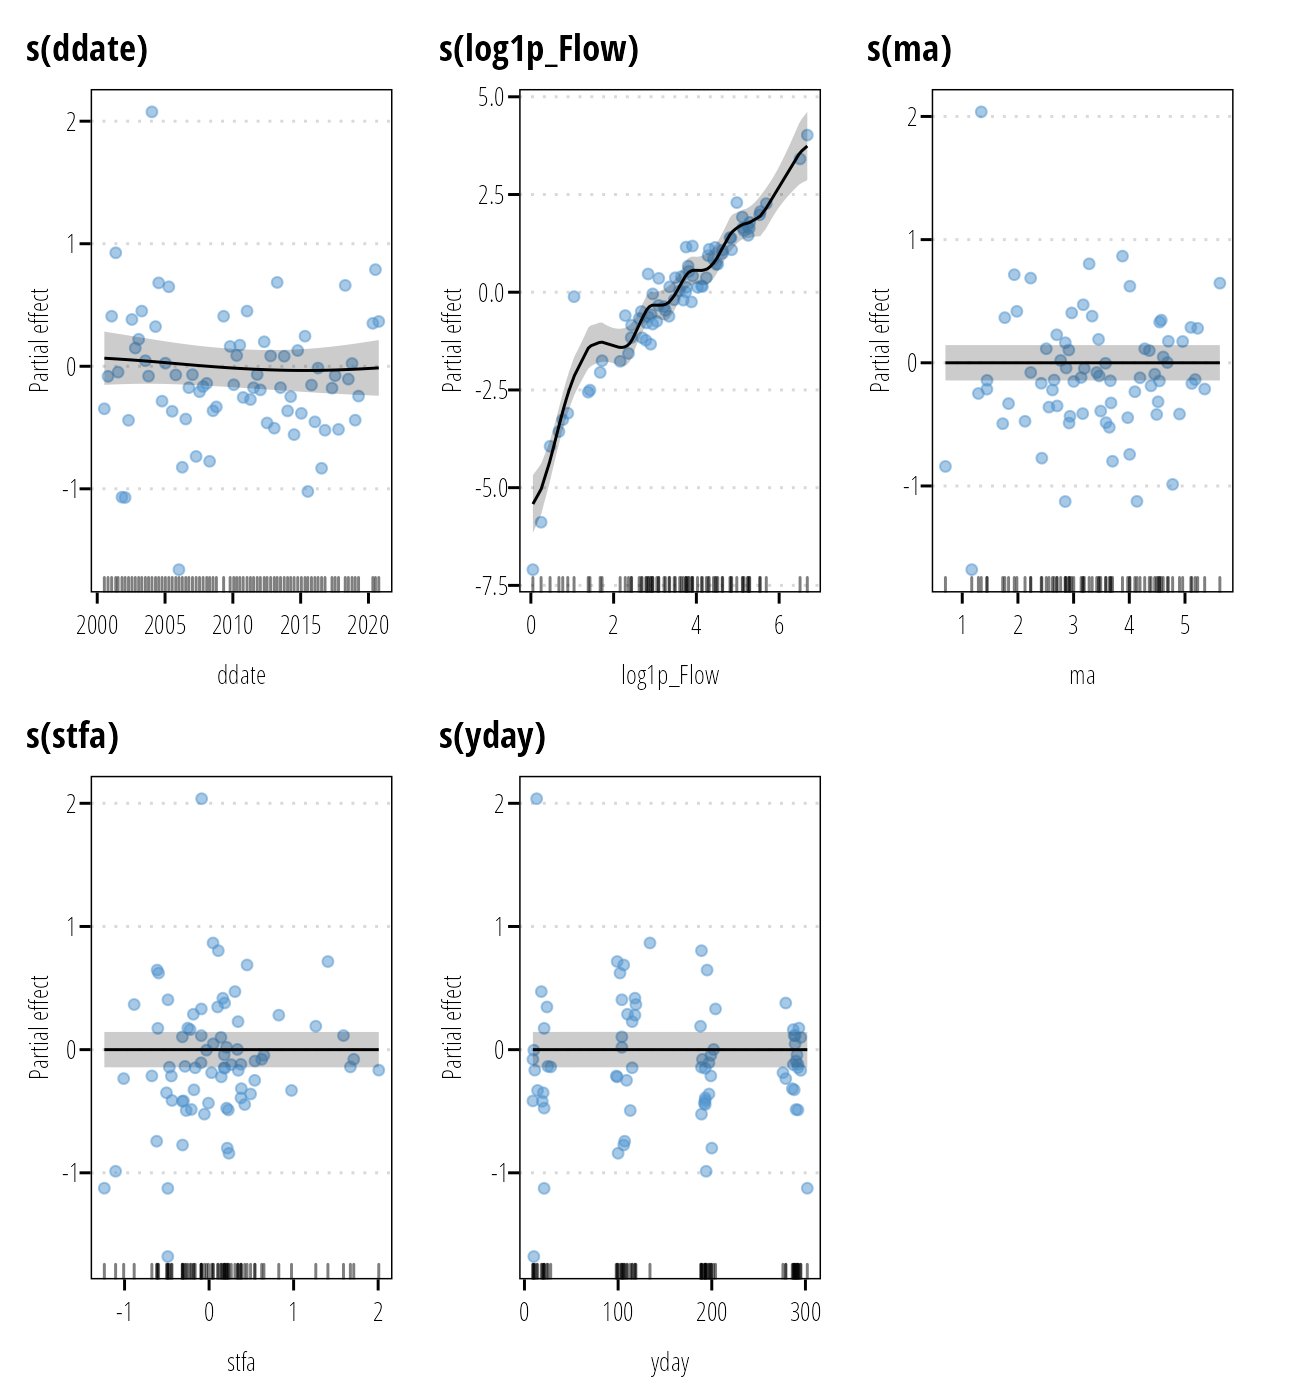
\includegraphics{model_assessment_files/figure-pdf/unnamed-chunk-35-1.png}

}

\caption{Partial effects of covariates in TP model at USGS-08164450.}

\end{figure}

\begin{figure}[h]

{\centering 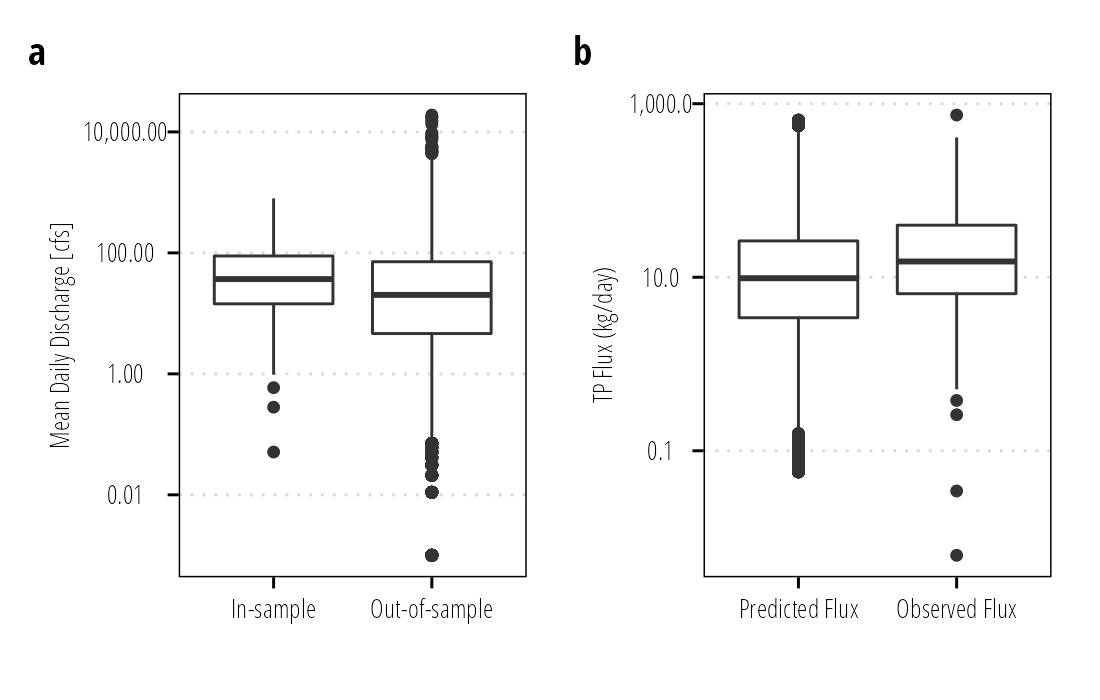
\includegraphics{model_assessment_files/figure-pdf/unnamed-chunk-36-1.png}

}

\caption{Comparisons of (a) in-sample and out-of-sample mean daily
discharge and (b) predicted daily fluxes (for both sampled and
non-sampled days) and measured daily fluxes.}

\end{figure}

\begin{figure}[h]

{\centering 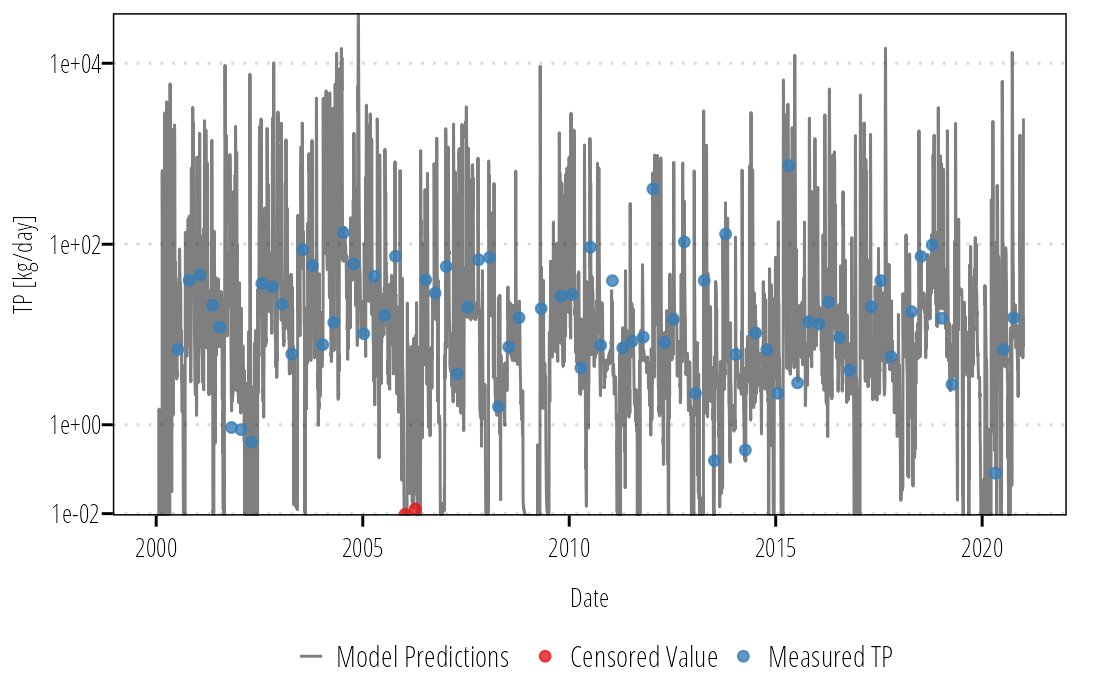
\includegraphics{model_assessment_files/figure-pdf/unnamed-chunk-37-1.png}

}

\caption{Time series plot of TP model predictions and observed values at
USGS-08164450.}

\end{figure}

\clearpage

\hypertarget{e-mustang-creek-nr-louise-usgs-08164504}{%
\subsection{E Mustang Creek nr Louise,
USGS-08164504}\label{e-mustang-creek-nr-louise-usgs-08164504}}

\hypertarget{no3-2}{%
\subsubsection{\texorpdfstring{NO\textsubscript{3}}{NO3}}\label{no3-2}}

\begin{widestuff}

\caption{NO\textsubscript{3}-N GAM summary - E Mustang Creek nr Louise, USGS-08164504.}
\centering
\begin{tabular}[t]{llllllrll}
\toprule
Component & Term & Estimate & Std.Error & t-value & edf & ref.df & F-value & p-value\textsuperscript{1}\\
\midrule
A. parametric coefficients & (Intercept) & -0.481 & 0.159 & -3.029 &  &  &  & 0.004 **\\
\cmidrule{1-9}
 & s(ddate) &  &  &  & 0.000 & 17 & 0.000 & 0.788\\

 & s(yday) &  &  &  & 2.557 & 4 & 6.592 & 0.000 ***\\

 & s(log1p(Flow)) &  &  &  & 2.793 & 4 & 3.688 & 0.001 **\\

 & s(ma) &  &  &  & 0.000 & 5 & 0.000 & 0.684\\

\multirow[t]{-5}{*}{\raggedright\arraybackslash B. smooth terms} & s(stfa) &  &  &  & 0.003 & 4 & 0.000 & 0.529\\
\bottomrule
\multicolumn{9}{l}{\textsuperscript{1} Signif. codes: 0 <= '***' < 0.001 < '**' < 0.01 < '*' < 0.05 < '+' < 0.1}\\
\multicolumn{9}{l}{\textsuperscript{} Adjusted R-squared: 0.348, Deviance explained 0.498}\\
\multicolumn{9}{l}{\textsuperscript{} -REML : 43.671, Scale est: 1.541, N: 61}\\
\end{tabular}
\end{widestuff}

\hypertarget{tbl-NO308164504-CV}{}
\begin{longtable}[]{@{}lc@{}}
\caption{\label{tbl-NO308164504-CV}Summary of goodness-of-fit metrics
for 5-fold cross-validation of NO\textsubscript{3}-N load GAM at E
Mustang Creek nr Louise, USGS-08164504.}\tabularnewline
\toprule()
\textbf{Goodness of Fit Metric} & \textbf{Median (IQR)} \\
\midrule()
\endfirsthead
\toprule()
\textbf{Goodness of Fit Metric} & \textbf{Median (IQR)} \\
\midrule()
\endhead
KGE & 0.37 (0.26, 0.41) \\
R\textsuperscript{2} & 0.54 (0.48, 0.57) \\
Percent Bias & -47 (-54, -44) \\
\bottomrule()
\end{longtable}

\clearpage

\begin{figure}[h]

{\centering 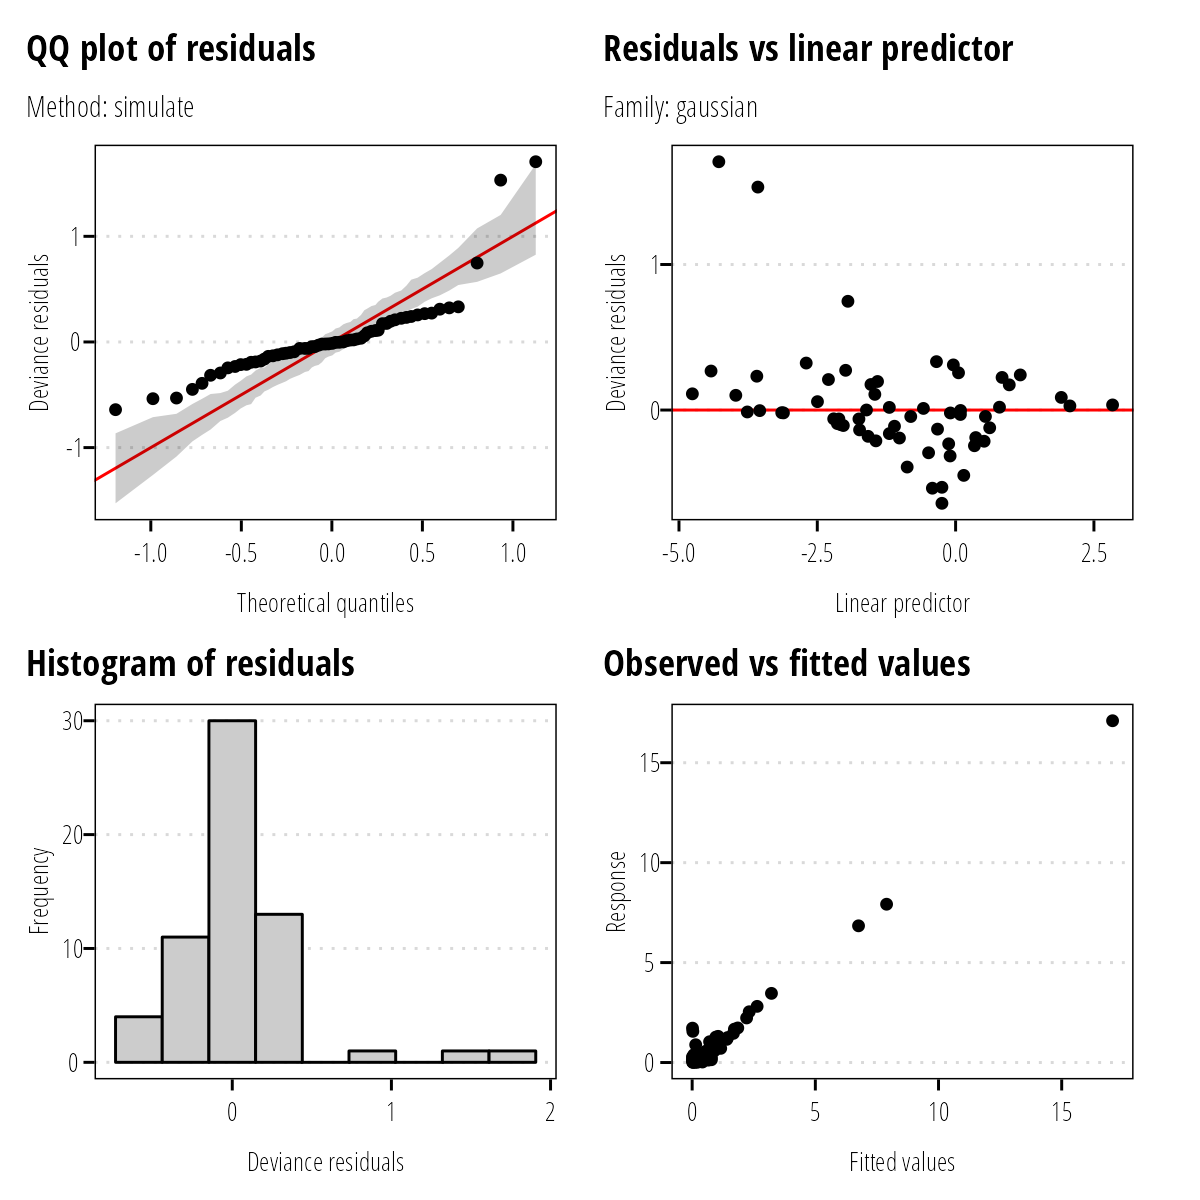
\includegraphics{model_assessment_files/figure-pdf/unnamed-chunk-40-1.png}

}

\caption{Diagnostic plot for NO\textsubscript{3} model at USGS-08164504}

\end{figure}

\begin{figure}[h]

{\centering 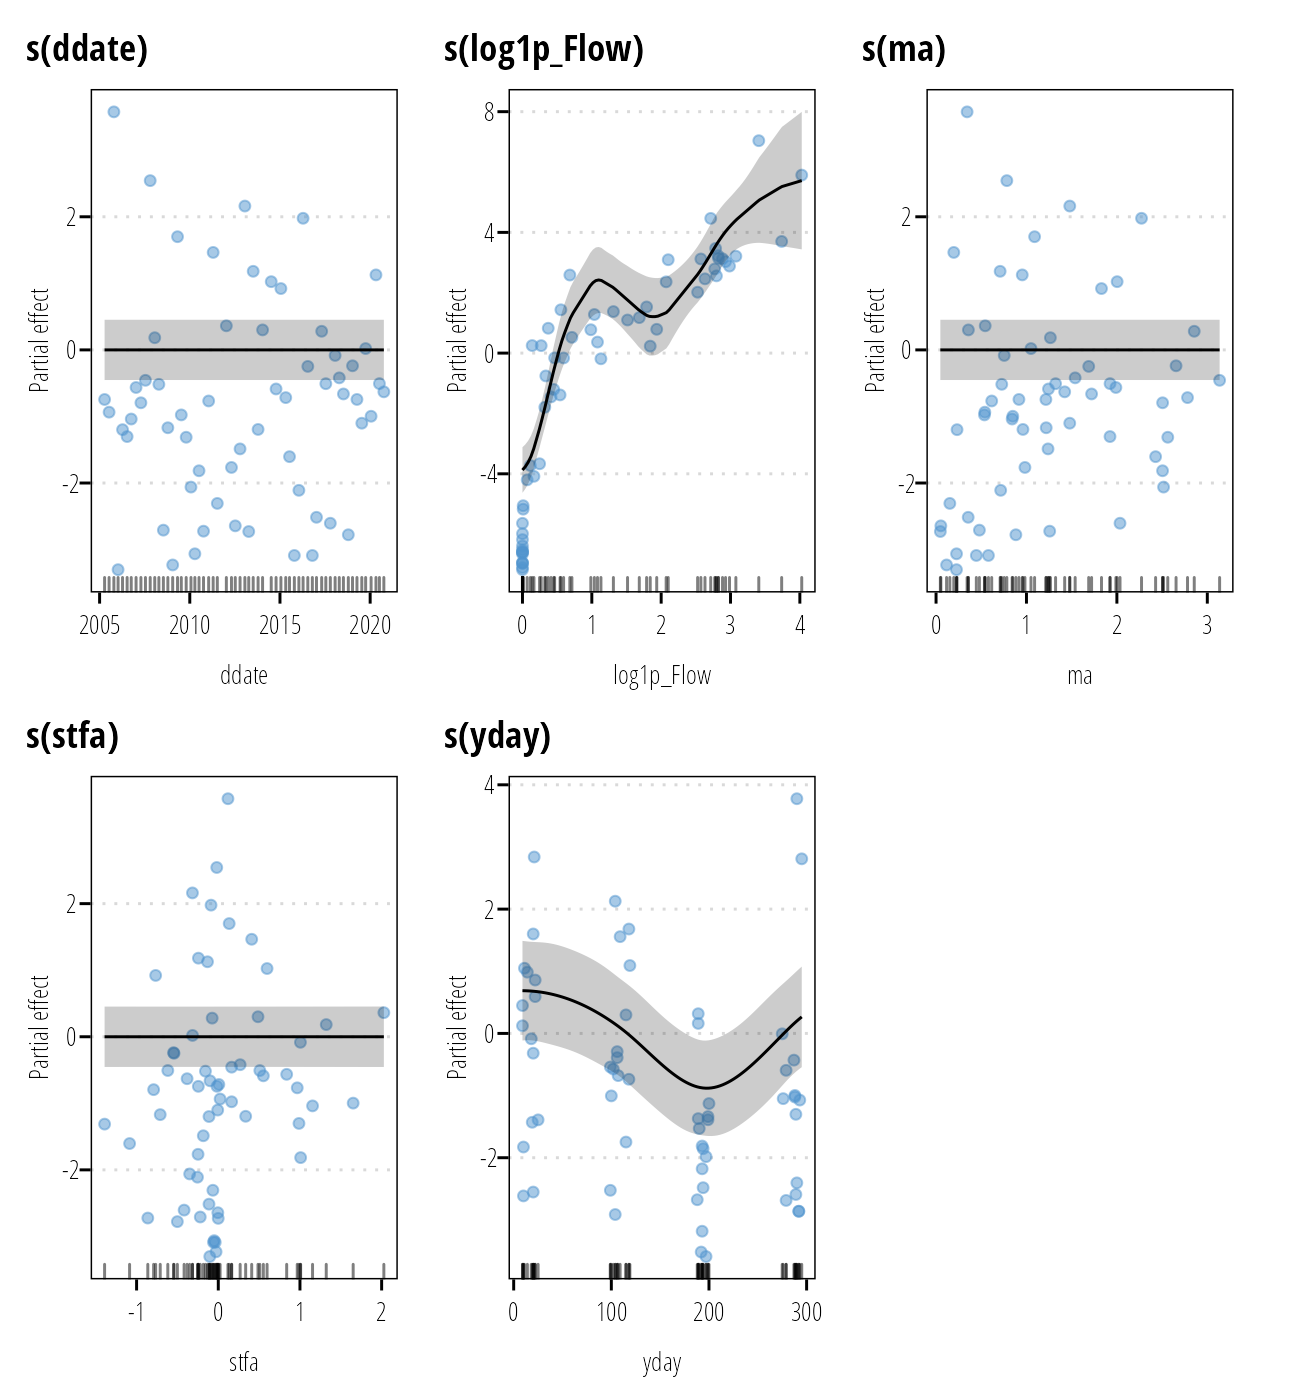
\includegraphics{model_assessment_files/figure-pdf/unnamed-chunk-41-1.png}

}

\caption{Partial effects of covariates in NO\textsubscript{3}-N model at
USGS-08164504}

\end{figure}

\begin{figure}[h]

{\centering 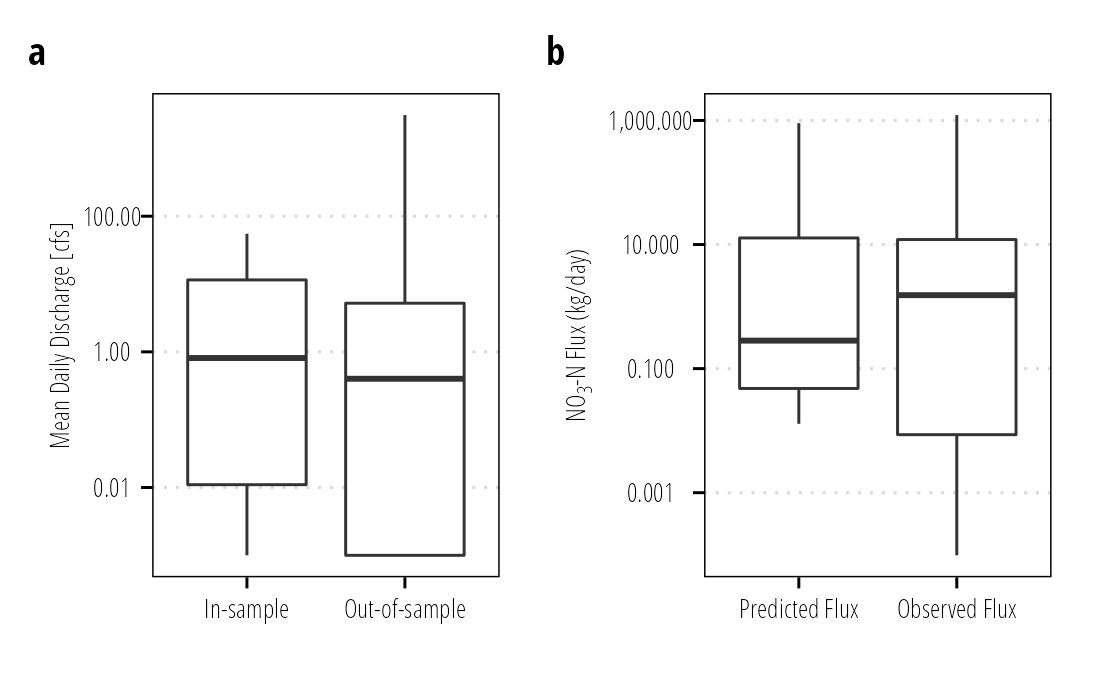
\includegraphics{model_assessment_files/figure-pdf/unnamed-chunk-42-1.png}

}

\caption{Comparisons of (a) in-sample and out-of-sample mean daily
discharge and (b) predicted daily fluxes (for both sampled and
non-sampled days) and measured daily fluxes.}

\end{figure}

\begin{figure}[h]

{\centering 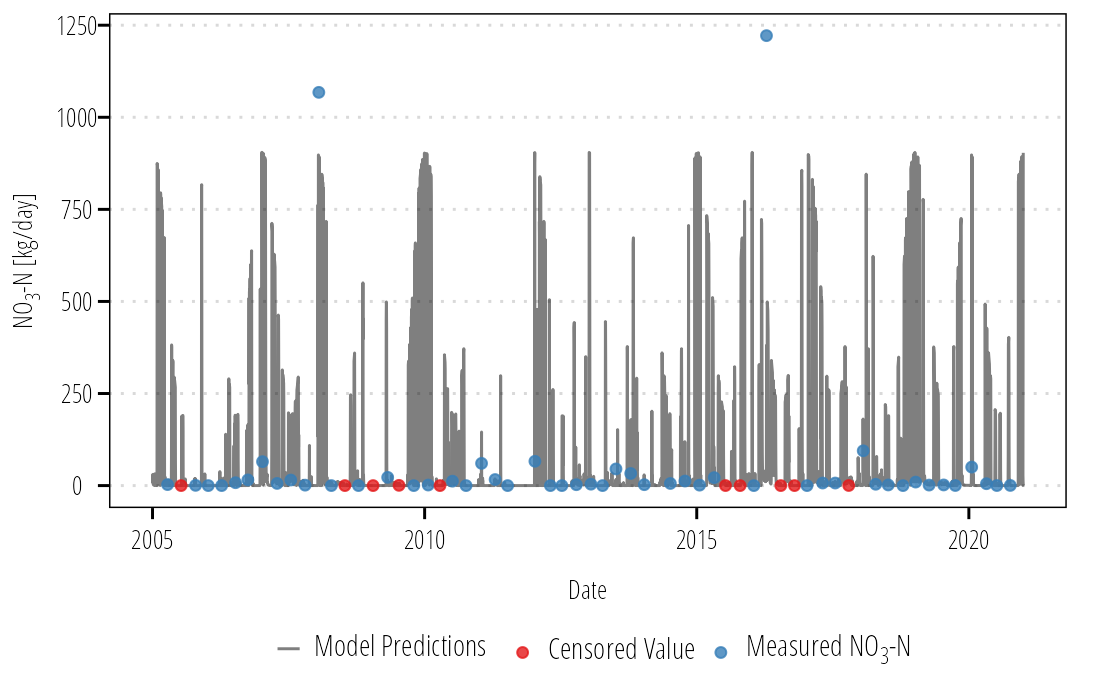
\includegraphics{model_assessment_files/figure-pdf/unnamed-chunk-43-1.png}

}

\caption{Time series plot of NO\textsubscript{3} model predictions and
observed values at USGS-08164504}

\end{figure}

\clearpage

\hypertarget{tp-3}{%
\subsubsection{TP}\label{tp-3}}

\begin{widestuff}

\caption{TP GAM summary - E Mustang Creek nr Louise, USGS-08164504.}
\centering
\begin{tabular}[t]{llllllrll}
\toprule
Component & Term & Estimate & Std.Error & t-value & edf & ref.df & F-value & p-value\textsuperscript{1}\\
\midrule
A. parametric coefficients & (Intercept) & -1.001 & 0.081 & -12.331 &  &  &  & 0.000 ***\\
\cmidrule{1-9}
 & s(ddate) &  &  &  & 0.044 & 17 & 0.003 & 0.343\\

 & s(yday) &  &  &  & 0.385 & 8 & 0.057 & 0.293\\

 & s(log1p(Flow)) &  &  &  & 1.642 & 4 & 1.416 & 0.005 **\\

 & s(ma) &  &  &  & 1.184 & 5 & 0.447 & 0.086 +\\

\multirow[t]{-5}{*}{\raggedright\arraybackslash B. smooth terms} & s(stfa) &  &  &  & 1.015 & 4 & 0.415 & 0.117\\
\bottomrule
\multicolumn{9}{l}{\textsuperscript{1} Signif. codes: 0 <= '***' < 0.001 < '**' < 0.01 < '*' < 0.05 < '+' < 0.1}\\
\multicolumn{9}{l}{\textsuperscript{} Adjusted R-squared: 0.263, Deviance explained 0.246}\\
\multicolumn{9}{l}{\textsuperscript{} -REML : -2.438, Scale est: 0.521, N: 79}\\
\end{tabular}
\end{widestuff}

\hypertarget{tbl-TP08164504-CV}{}
\begin{longtable}[]{@{}lc@{}}
\caption{\label{tbl-TP08164504-CV}Summary of goodness-of-fit metrics for
5-fold cross-validation of TP load GAM at E Mustang Creek nr Louise,
USGS-08164504.}\tabularnewline
\toprule()
\textbf{Goodness of Fit Metric} & \textbf{Median (IQR)} \\
\midrule()
\endfirsthead
\toprule()
\textbf{Goodness of Fit Metric} & \textbf{Median (IQR)} \\
\midrule()
\endhead
KGE & 0.851 (0.812, 0.855) \\
R\textsuperscript{2} & 0.854 (0.839, 0.859) \\
Percent Bias & -9.2 (-12.7, -7.5) \\
\bottomrule()
\end{longtable}

\clearpage

\begin{figure}[h]

{\centering 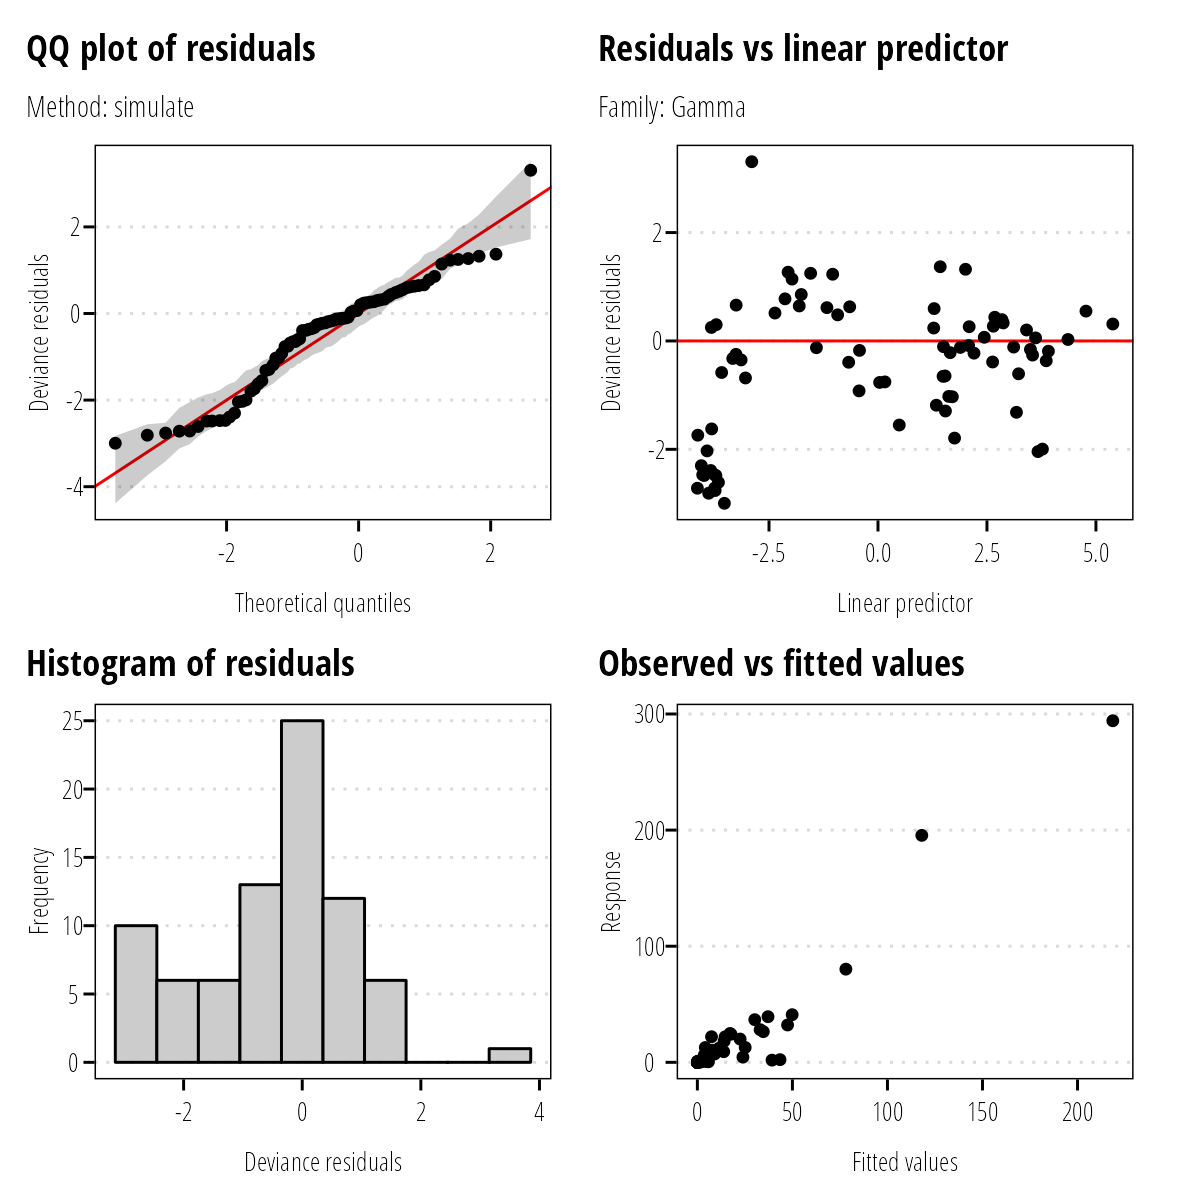
\includegraphics{model_assessment_files/figure-pdf/unnamed-chunk-46-1.png}

}

\caption{Diagnostic plot for TP model at USGS-08164504}

\end{figure}

\begin{figure}[h]

{\centering 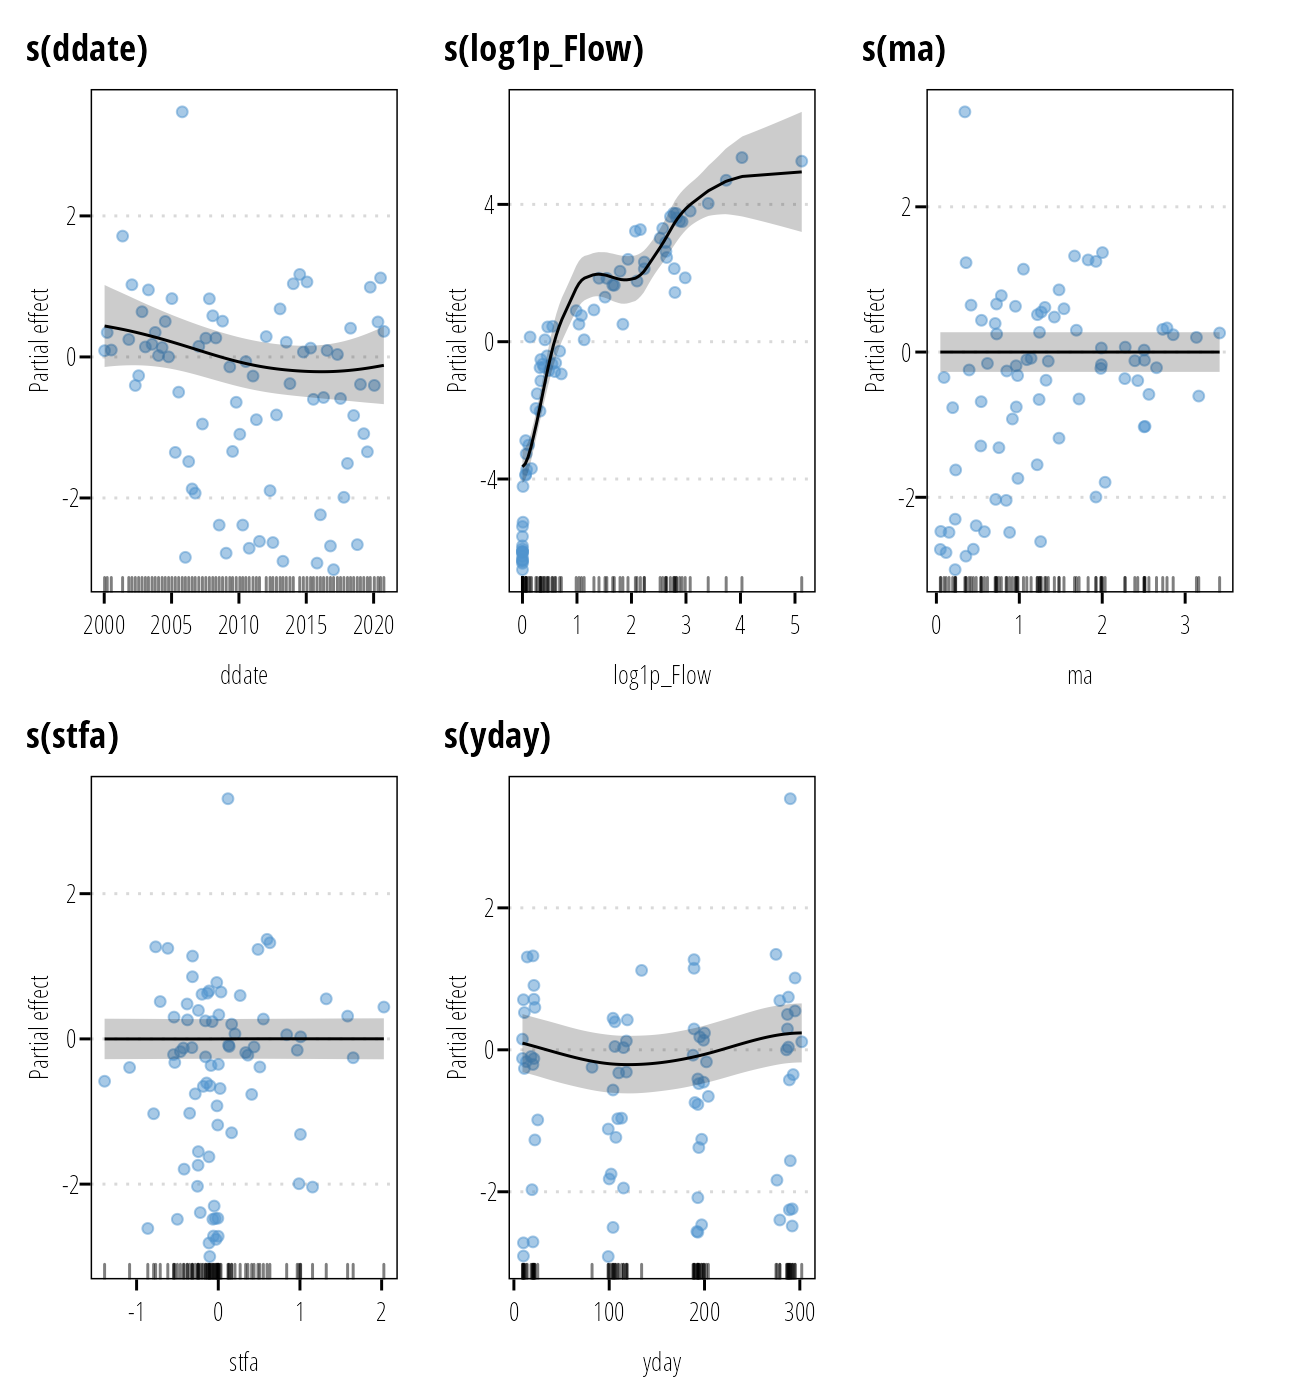
\includegraphics{model_assessment_files/figure-pdf/unnamed-chunk-47-1.png}

}

\caption{Partial effects of covariates in TP model at USGS-08164504}

\end{figure}

\begin{figure}[h]

{\centering 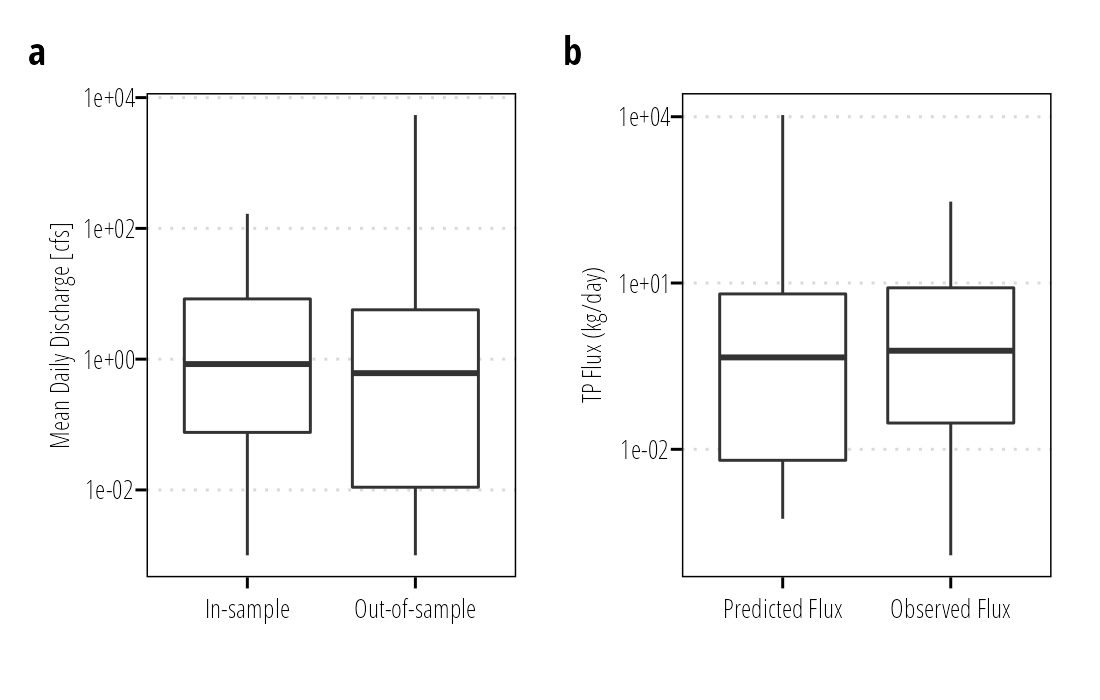
\includegraphics{model_assessment_files/figure-pdf/unnamed-chunk-48-1.png}

}

\caption{Comparisons of (a) in-sample and out-of-sample mean daily
discharge and (b) predicted daily fluxes (for both sampled and
non-sampled days) and measured daily fluxes.}

\end{figure}

\begin{figure}[h]

{\centering 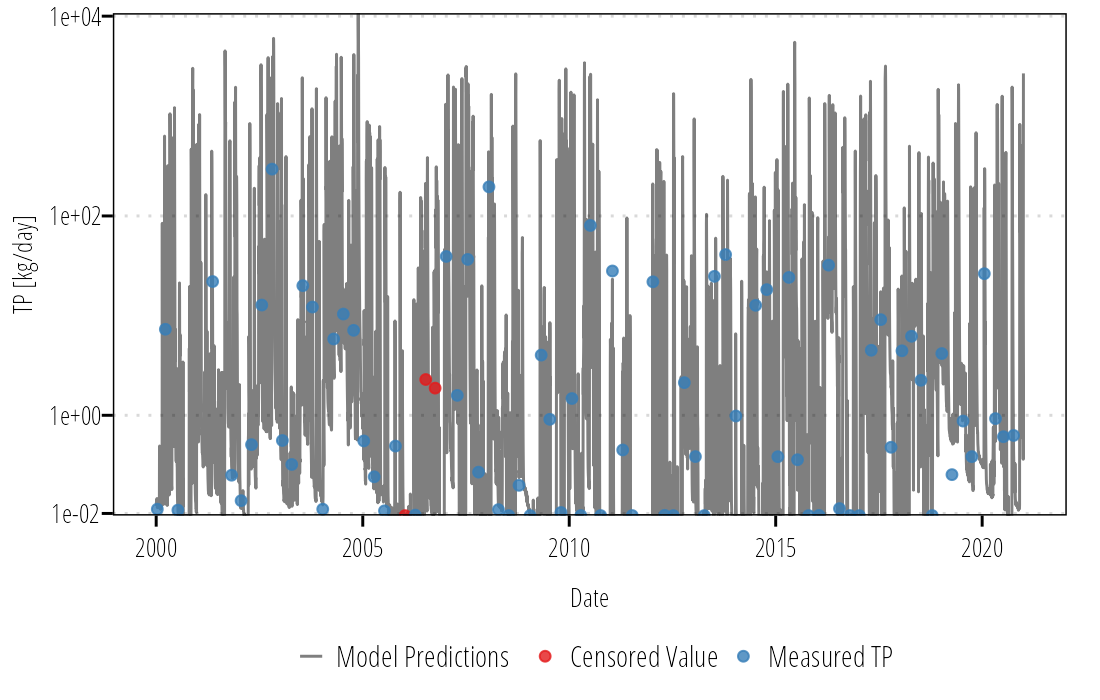
\includegraphics{model_assessment_files/figure-pdf/unnamed-chunk-49-1.png}

}

\caption{Time series plot of TP model predictions and observed values at
USGS-08164504}

\end{figure}

\clearpage

\hypertarget{w-mustang-creek-nr-ganado-usgs-08164503}{%
\subsection{W Mustang Creek nr Ganado,
USGS-08164503}\label{w-mustang-creek-nr-ganado-usgs-08164503}}

\hypertarget{no3-3}{%
\subsubsection{\texorpdfstring{NO\textsubscript{3}}{NO3}}\label{no3-3}}

\begin{widestuff}

\caption{NO\textsubscript{3}-N GAM summary - W Mustang Creek nr Ganado, USGS-08164503.}
\centering
\begin{tabular}[t]{llllllrll}
\toprule
Component & Term & Estimate & Std.Error & t-value & edf & ref.df & F-value & p-value\textsuperscript{1}\\
\midrule
A. parametric coefficients & (Intercept) & -1.217 & 0.085 & -14.372 &  &  &  & 0.000 ***\\
\cmidrule{1-9}
 & s(ddate) &  &  &  & 1.161 & 17 & 0.210 & 0.048 *\\

 & s(yday) &  &  &  & 2.554 & 4 & 8.892 & 0.000 ***\\

 & s(log1p(Flow)) &  &  &  & 5.355 & 6 & 7.166 & 0.000 ***\\

 & s(ma) &  &  &  & 0.855 & 5 & 0.267 & 0.151\\

\multirow[t]{-5}{*}{\raggedright\arraybackslash B. smooth terms} & s(stfa) &  &  &  & 1.272 & 5 & 0.352 & 0.199\\
\bottomrule
\multicolumn{9}{l}{\textsuperscript{1} Signif. codes: 0 <= '***' < 0.001 < '**' < 0.01 < '*' < 0.05 < '+' < 0.1}\\
\multicolumn{9}{l}{\textsuperscript{} Adjusted R-squared: 0.566, Deviance explained 0.632}\\
\multicolumn{9}{l}{\textsuperscript{} -REML : -2.104, Scale est: 0.452, N: 63}\\
\end{tabular}
\end{widestuff}

\hypertarget{tbl-NO08164503-CV}{}
\begin{longtable}[]{@{}lc@{}}
\caption{\label{tbl-NO08164503-CV}Summary of goodness-of-fit metrics for
5-fold cross-validation of NO\textsubscript{3}-N load GAM at W Mustang
Creek nr Ganado, USGS-08164503.}\tabularnewline
\toprule()
\textbf{Goodness of Fit Metric} & \textbf{Median (IQR)} \\
\midrule()
\endfirsthead
\toprule()
\textbf{Goodness of Fit Metric} & \textbf{Median (IQR)} \\
\midrule()
\endhead
KGE & 0.51 (0.32, 0.69) \\
R\textsuperscript{2} & 0.55 (0.44, 0.70) \\
Percent Bias & -17 (-22, -11) \\
\bottomrule()
\end{longtable}

\clearpage

\begin{figure}[h]

{\centering 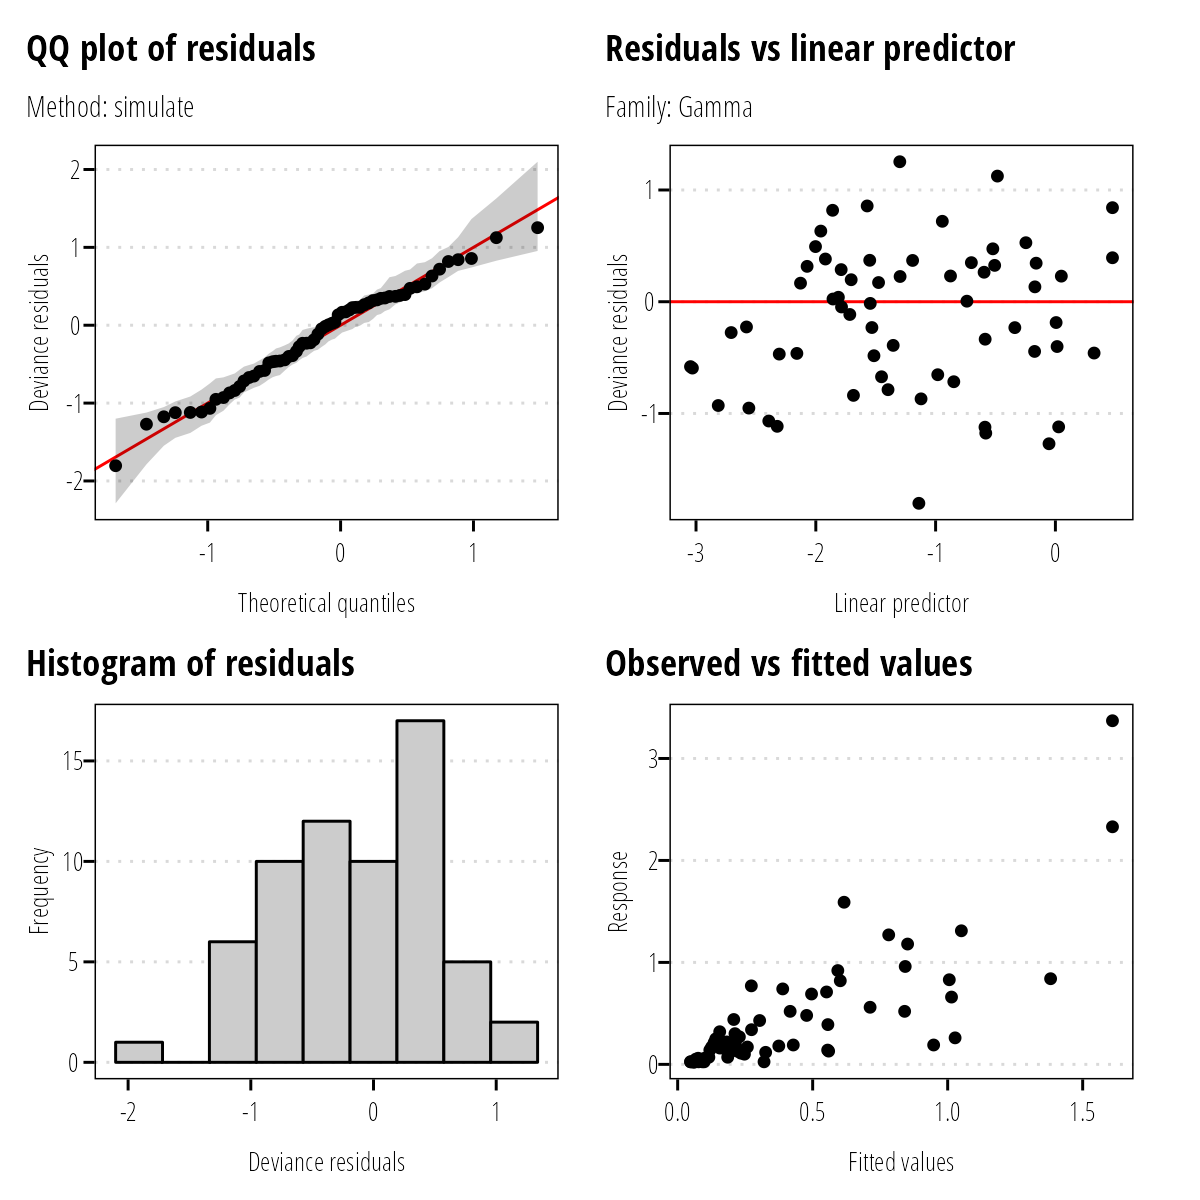
\includegraphics{model_assessment_files/figure-pdf/unnamed-chunk-52-1.png}

}

\caption{Diagnostic plot for NO\textsubscript{3} model at USGS-08164503}

\end{figure}

\begin{figure}[h]

{\centering 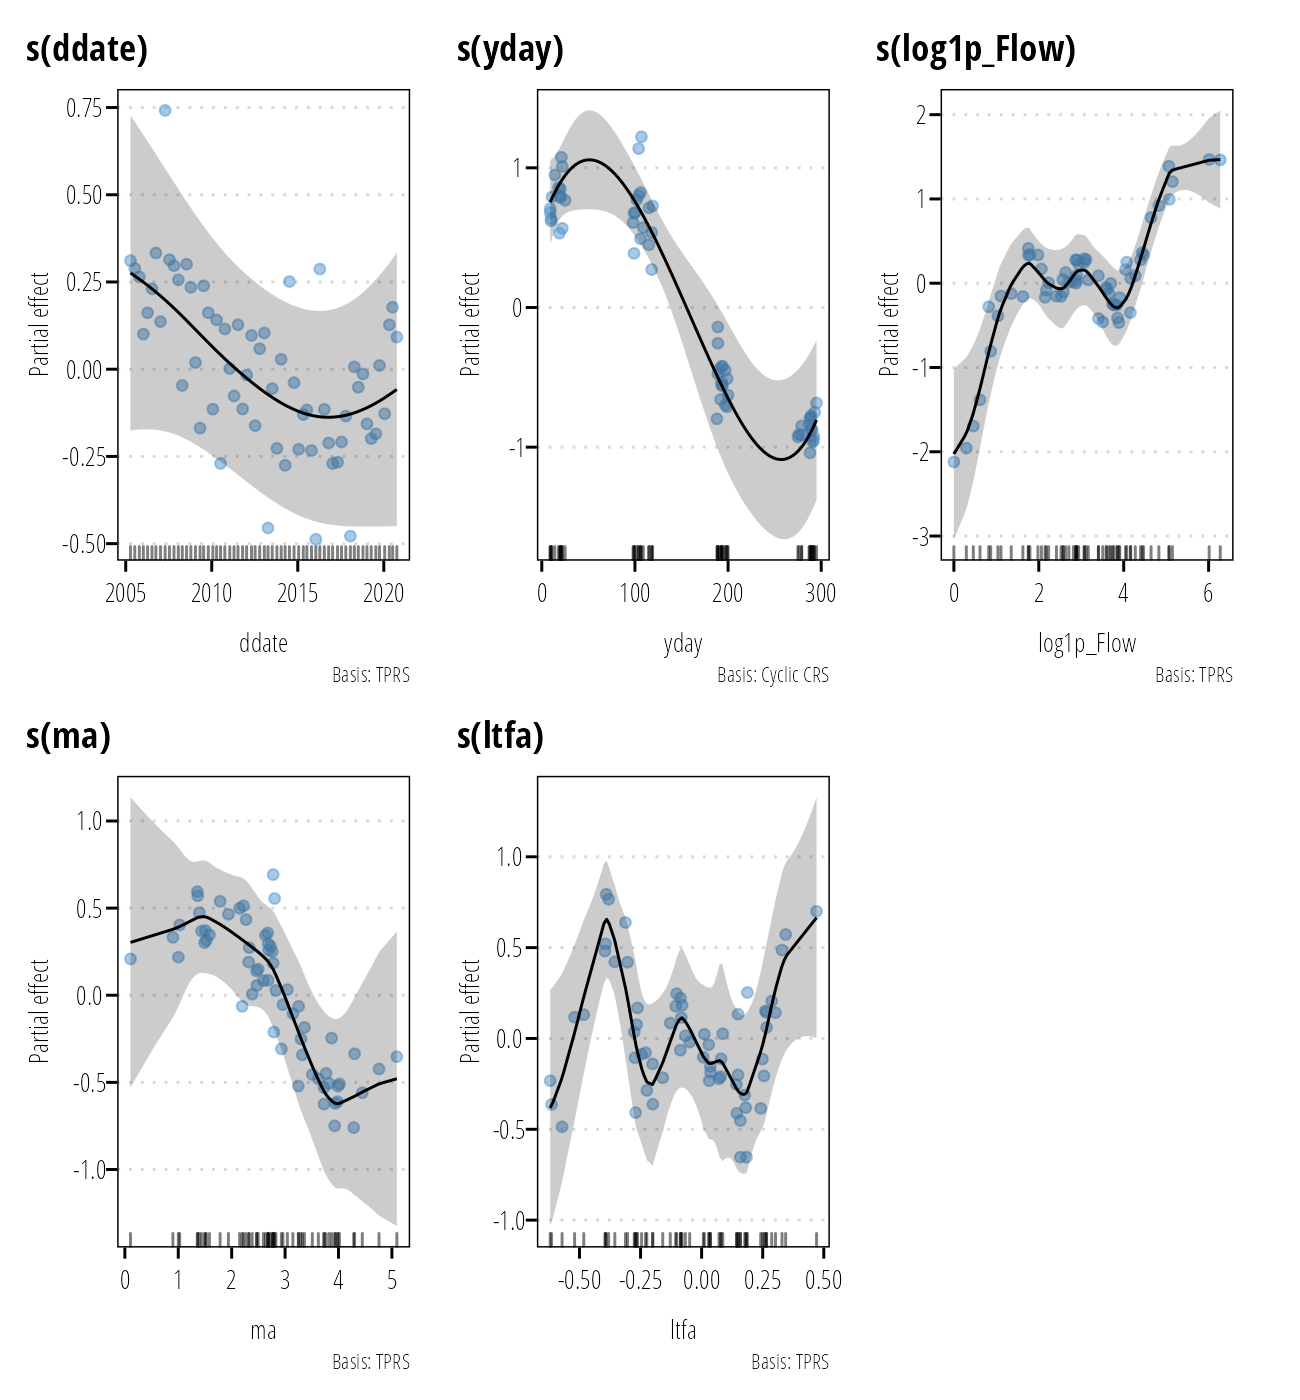
\includegraphics{model_assessment_files/figure-pdf/unnamed-chunk-53-1.png}

}

\caption{Partial effects of covariates in NO\textsubscript{3}-N model at
USGS-08164503}

\end{figure}

\begin{figure}[h]

{\centering 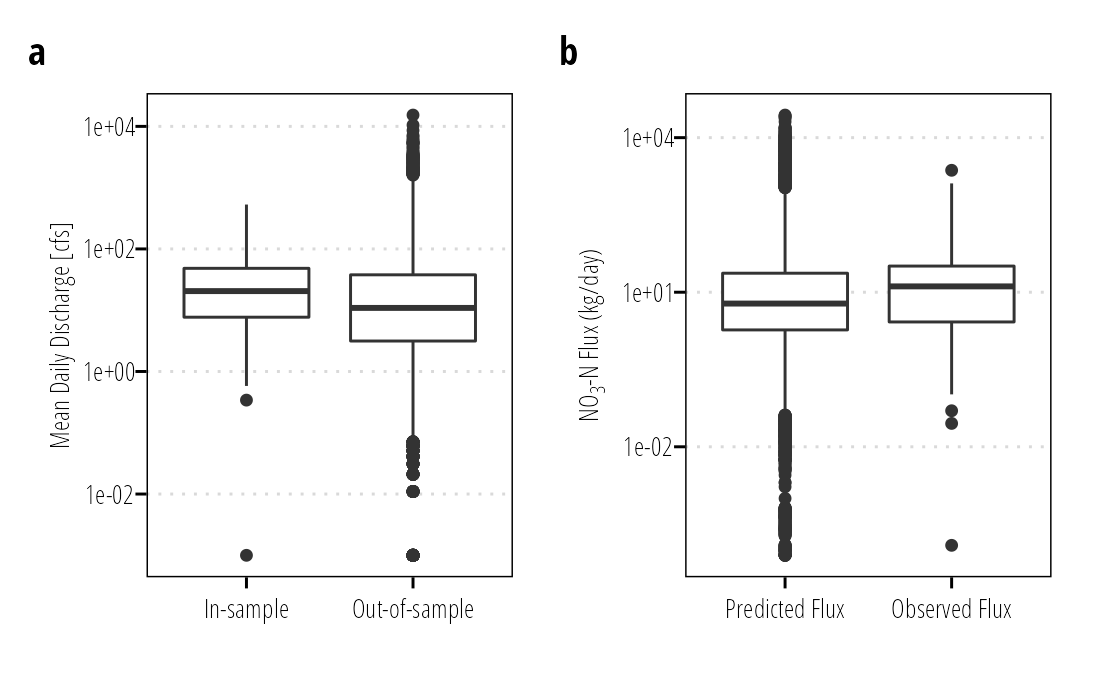
\includegraphics{model_assessment_files/figure-pdf/unnamed-chunk-54-1.png}

}

\caption{Comparisons of (a) in-sample and out-of-sample mean daily
discharge and (b) predicted daily fluxes (for both sampled and
non-sampled days) and measured daily fluxes.}

\end{figure}

\begin{figure}[h]

{\centering 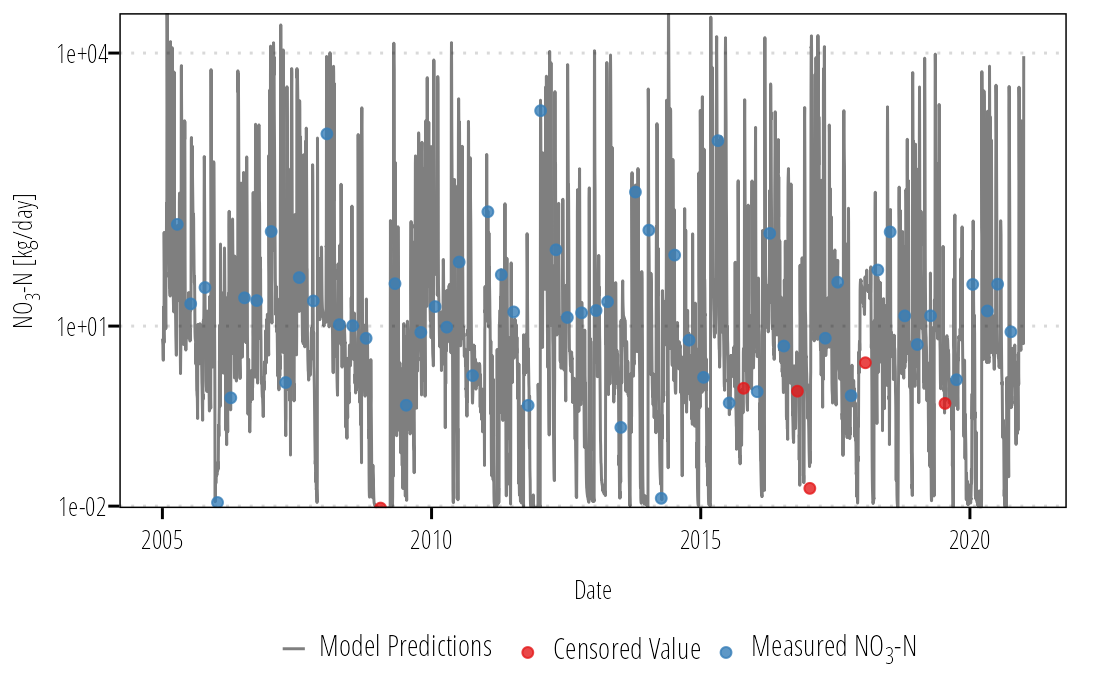
\includegraphics{model_assessment_files/figure-pdf/unnamed-chunk-55-1.png}

}

\caption{Time series plot of NO\textsubscript{3} model predictions and
observed values at USGS-08164503}

\end{figure}

\clearpage

\hypertarget{tp-4}{%
\subsubsection{TP}\label{tp-4}}

\begin{widestuff}

\caption{TP GAM summary - W Mustang Creek nr Ganado, USGS-08164503.}
\centering
\begin{tabular}[t]{llllllrll}
\toprule
Component & Term & Estimate & Std.Error & t-value & edf & ref.df & F-value & p-value\textsuperscript{1}\\
\midrule
A. parametric coefficients & (Intercept) & -1.150 & 0.063 & -18.148 &  &  &  & 0.000 ***\\
\cmidrule{1-9}
 & s(ddate) &  &  &  & 2.054 & 17 & 0.411 & 0.025 *\\

 & s(yday) &  &  &  & 0.000 & 4 & 0.000 & 0.573\\

 & s(log1p(Flow)) &  &  &  & 0.000 & 9 & 0.000 & 0.648\\

 & s(stfa) &  &  &  & 0.235 & 5 & 0.050 & 0.342\\

\multirow[t]{-5}{*}{\raggedright\arraybackslash B. smooth terms} & s(ma) &  &  &  & 0.285 & 5 & 0.067 & 0.293\\
\bottomrule
\multicolumn{9}{l}{\textsuperscript{1} Signif. codes: 0 <= '***' < 0.001 < '**' < 0.01 < '*' < 0.05 < '+' < 0.1}\\
\multicolumn{9}{l}{\textsuperscript{} Adjusted R-squared: 0.0843, Deviance explained 0.142}\\
\multicolumn{9}{l}{\textsuperscript{} -REML : -33.755, Scale est: 0.325, N: 81}\\
\end{tabular}
\end{widestuff}

\hypertarget{tbl-TP08164503-CV}{}
\begin{longtable}[]{@{}lc@{}}
\caption{\label{tbl-TP08164503-CV}Summary of goodness-of-fit metrics for
5-fold cross-validation of TP load GAM at W Mustang Creek nr Ganado,
USGS-08164503.}\tabularnewline
\toprule()
\textbf{Goodness of Fit Metric} & \textbf{Median (IQR)} \\
\midrule()
\endfirsthead
\toprule()
\textbf{Goodness of Fit Metric} & \textbf{Median (IQR)} \\
\midrule()
\endhead
KGE & 0.864 (0.838, 0.882) \\
R\textsuperscript{2} & 0.890 (0.887, 0.896) \\
Percent Bias & -6.50 (-9.12, -4.70) \\
\bottomrule()
\end{longtable}

\clearpage

\begin{figure}[h]

{\centering 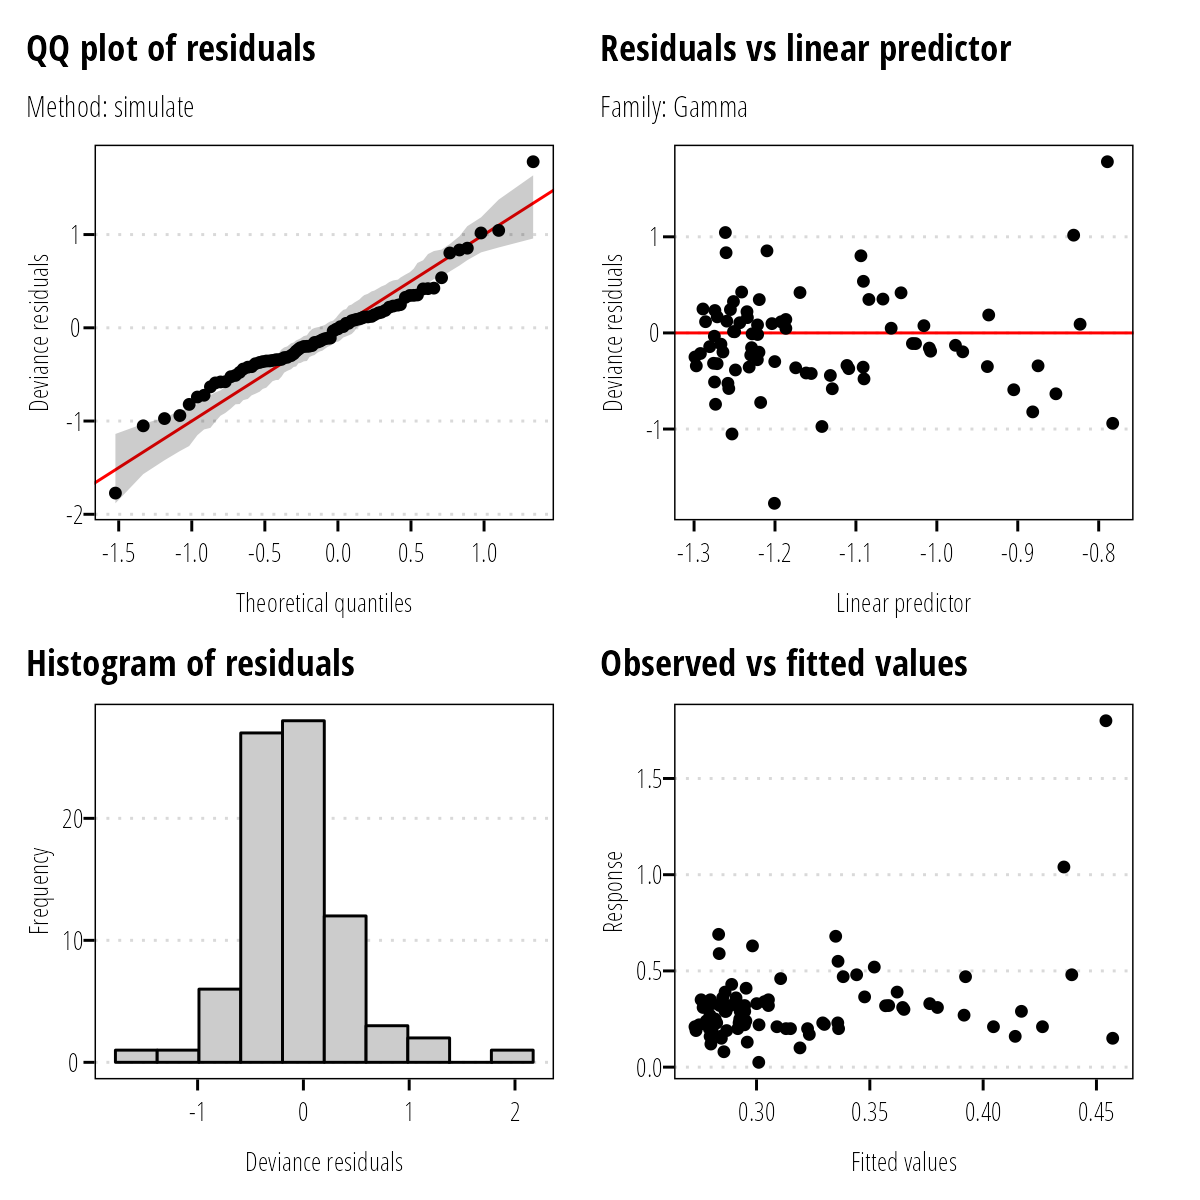
\includegraphics{model_assessment_files/figure-pdf/unnamed-chunk-58-1.png}

}

\caption{Diagnostic plot for TP model at USGS-08164503}

\end{figure}

\begin{figure}[h]

{\centering 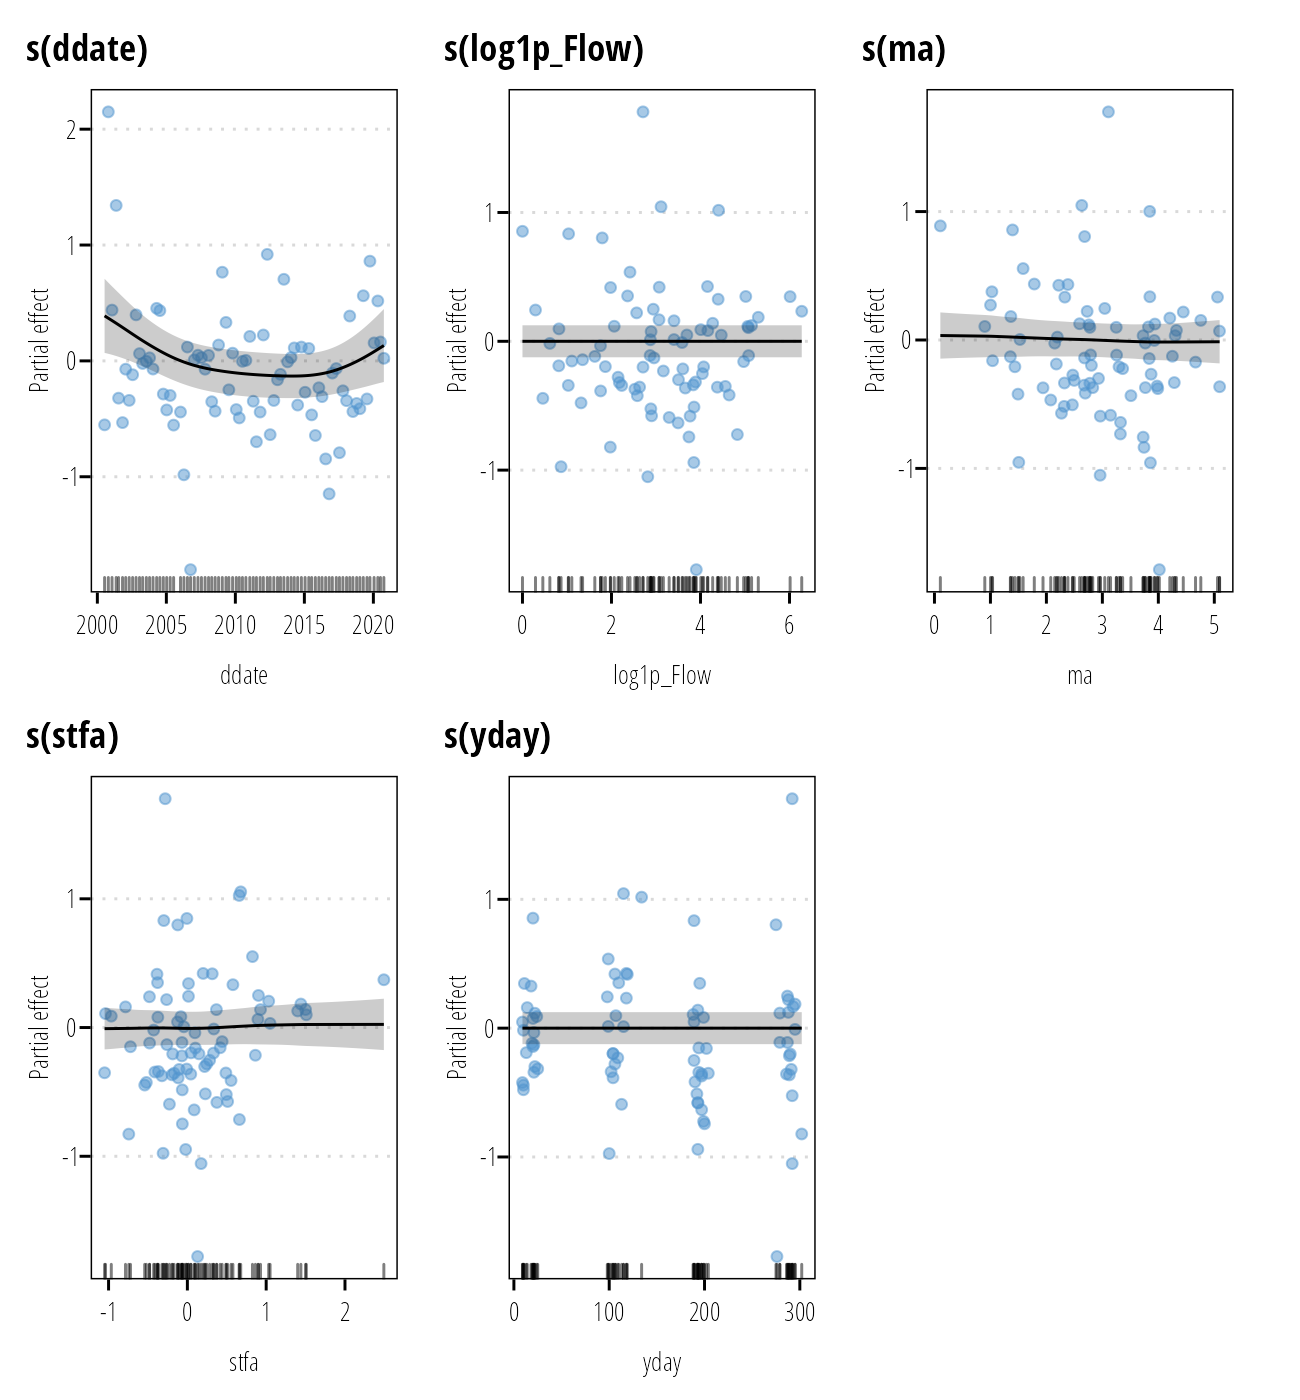
\includegraphics{model_assessment_files/figure-pdf/unnamed-chunk-59-1.png}

}

\caption{Partial effects of covariates in TP model at USGS-08164503}

\end{figure}

\begin{figure}[h]

{\centering 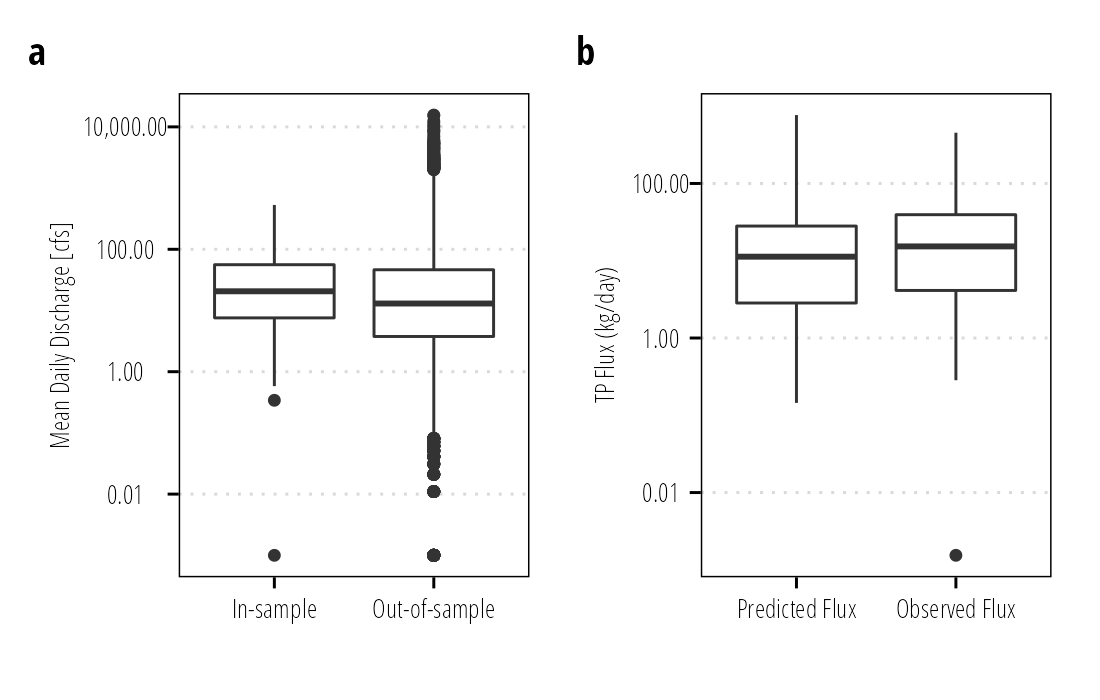
\includegraphics{model_assessment_files/figure-pdf/unnamed-chunk-60-1.png}

}

\caption{Comparisons of (a) in-sample and out-of-sample mean daily
discharge and (b) predicted daily fluxes (for both sampled and
non-sampled days) and measured daily fluxes.}

\end{figure}

\begin{figure}[h]

{\centering 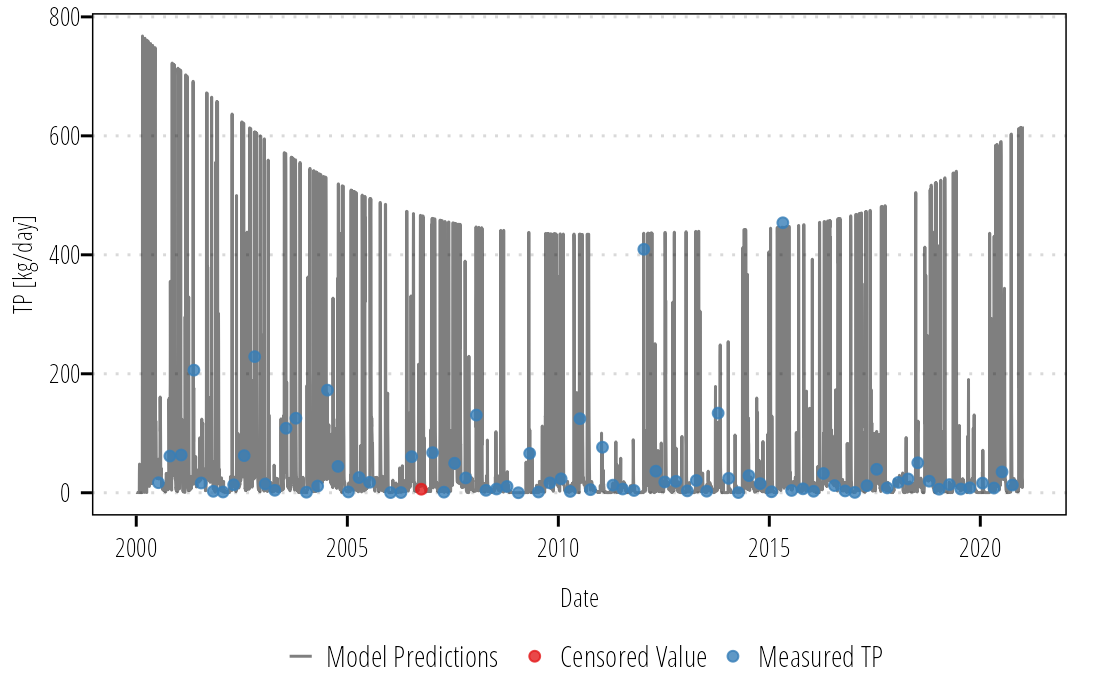
\includegraphics{model_assessment_files/figure-pdf/unnamed-chunk-61-1.png}

}

\caption{Time series plot of TP model predictions and observed values at
USGS-08164503}

\end{figure}

\clearpage

\hypertarget{palmetto-bend-dam}{%
\subsection{Palmetto Bend Dam}\label{palmetto-bend-dam}}

\hypertarget{no3-4}{%
\subsubsection{\texorpdfstring{NO\textsubscript{3}}{NO3}}\label{no3-4}}

\begin{widestuff}

\caption{NO\textsubscript{3}-N GAM summary - Navidad River at Palmetto Bend Dam.}
\centering
\begin{tabular}[t]{llllllrll}
\toprule
Component & Term & Estimate & Std.Error & t-value & edf & ref.df & F-value & p-value\textsuperscript{1}\\
\midrule
A. parametric coefficients & (Intercept) & -1.456 & 0.078 & -18.664 &  &  &  & 0.000 ***\\
\cmidrule{1-9}
 & s(ddate) &  &  &  & 11.783 & 14 & 3.702 & 0.000 ***\\

 & s(yday) &  &  &  & 2.924 & 8 & 6.812 & 0.000 ***\\

 & s(log1p(Inflow)) &  &  &  & 0.000 & 4 & 0.000 & 0.353\\

 & s(log1p(Flow)) &  &  &  & 2.804 & 9 & 1.303 & 0.002 **\\

 & s(stfa) &  &  &  & 1.154 & 4 & 0.619 & 0.070 +\\

\multirow[t]{-6}{*}{\raggedright\arraybackslash B. smooth terms} & s(ma) &  &  &  & 3.478 & 5 & 2.980 & 0.001 **\\
\bottomrule
\multicolumn{9}{l}{\textsuperscript{1} Signif. codes: 0 <= '***' < 0.001 < '**' < 0.01 < '*' < 0.05 < '+' < 0.1}\\
\multicolumn{9}{l}{\textsuperscript{} Adjusted R-squared: 0.811, Deviance explained 0.878}\\
\multicolumn{9}{l}{\textsuperscript{} -REML : -11.573, Scale est: 0.0128, N: 62}\\
\end{tabular}
\end{widestuff}

\hypertarget{tbl-NO3PalmettoBend-CV}{}
\begin{longtable}[]{@{}lc@{}}
\caption{\label{tbl-NO3PalmettoBend-CV}Summary of goodness-of-fit
metrics for 5-fold cross-validation of NO\textsubscript{3}-N load GAM at
Palmetto Bend Dam.}\tabularnewline
\toprule()
\textbf{Goodness of Fit Metric} & \textbf{Median (IQR)} \\
\midrule()
\endfirsthead
\toprule()
\textbf{Goodness of Fit Metric} & \textbf{Median (IQR)} \\
\midrule()
\endhead
KGE & 0.49 (0.31, 0.66) \\
R\textsuperscript{2} & 0.79 (0.69, 0.89) \\
Percent Bias & -43 (-57, -32) \\
\bottomrule()
\end{longtable}

\clearpage

\begin{figure}[h]

{\centering 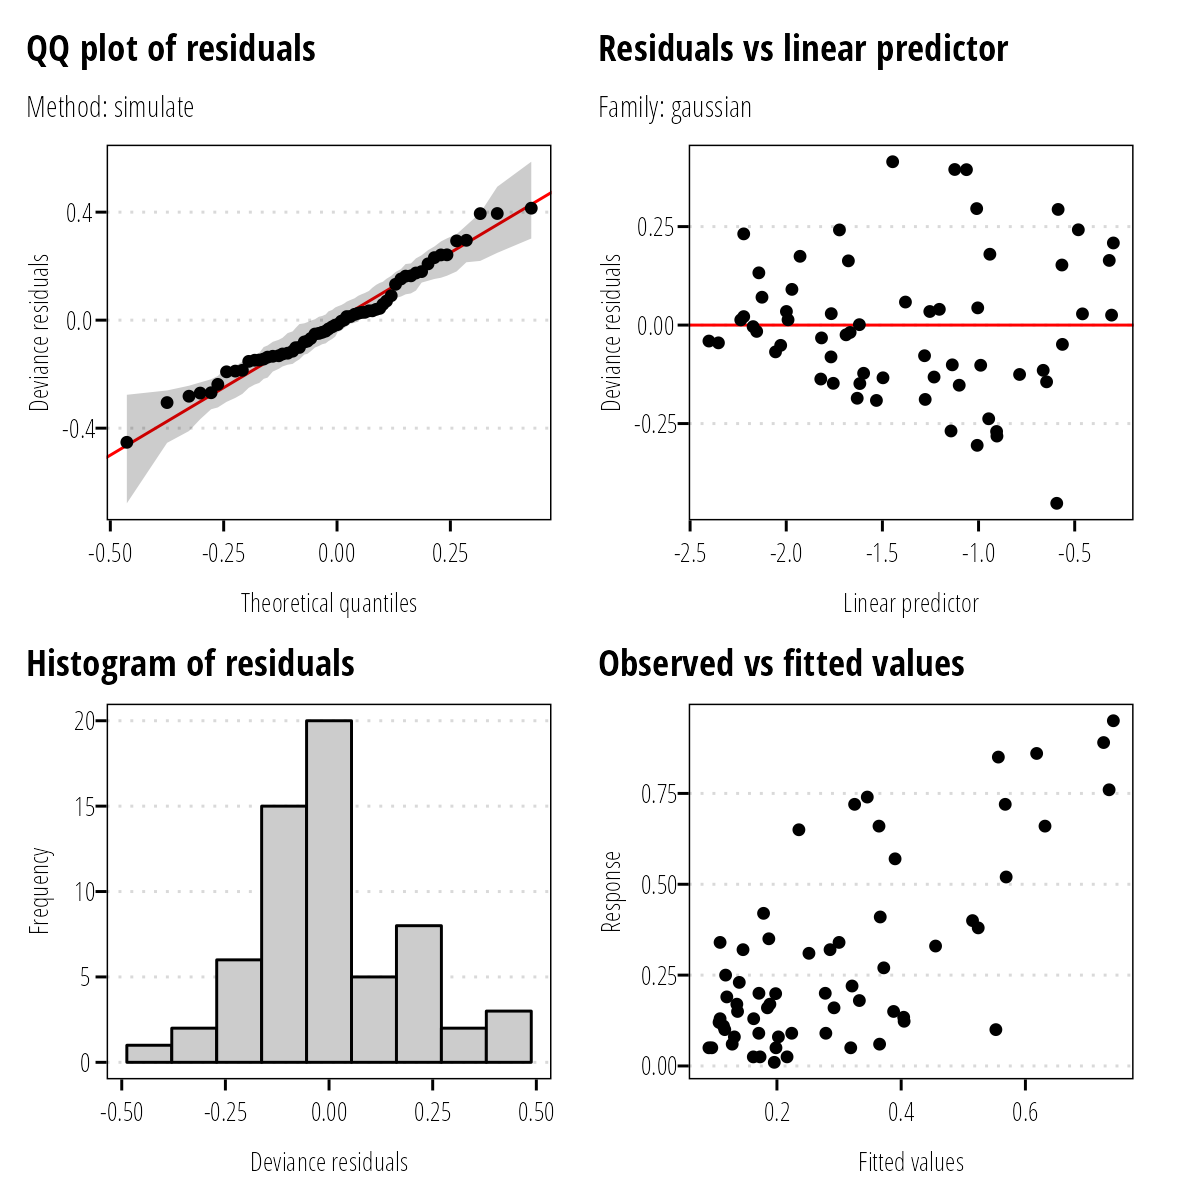
\includegraphics{model_assessment_files/figure-pdf/unnamed-chunk-64-1.png}

}

\caption{Diagnostic plot for NO\textsubscript{3} model below Palmetto
Bend Dam.}

\end{figure}

\begin{figure}[h]

{\centering 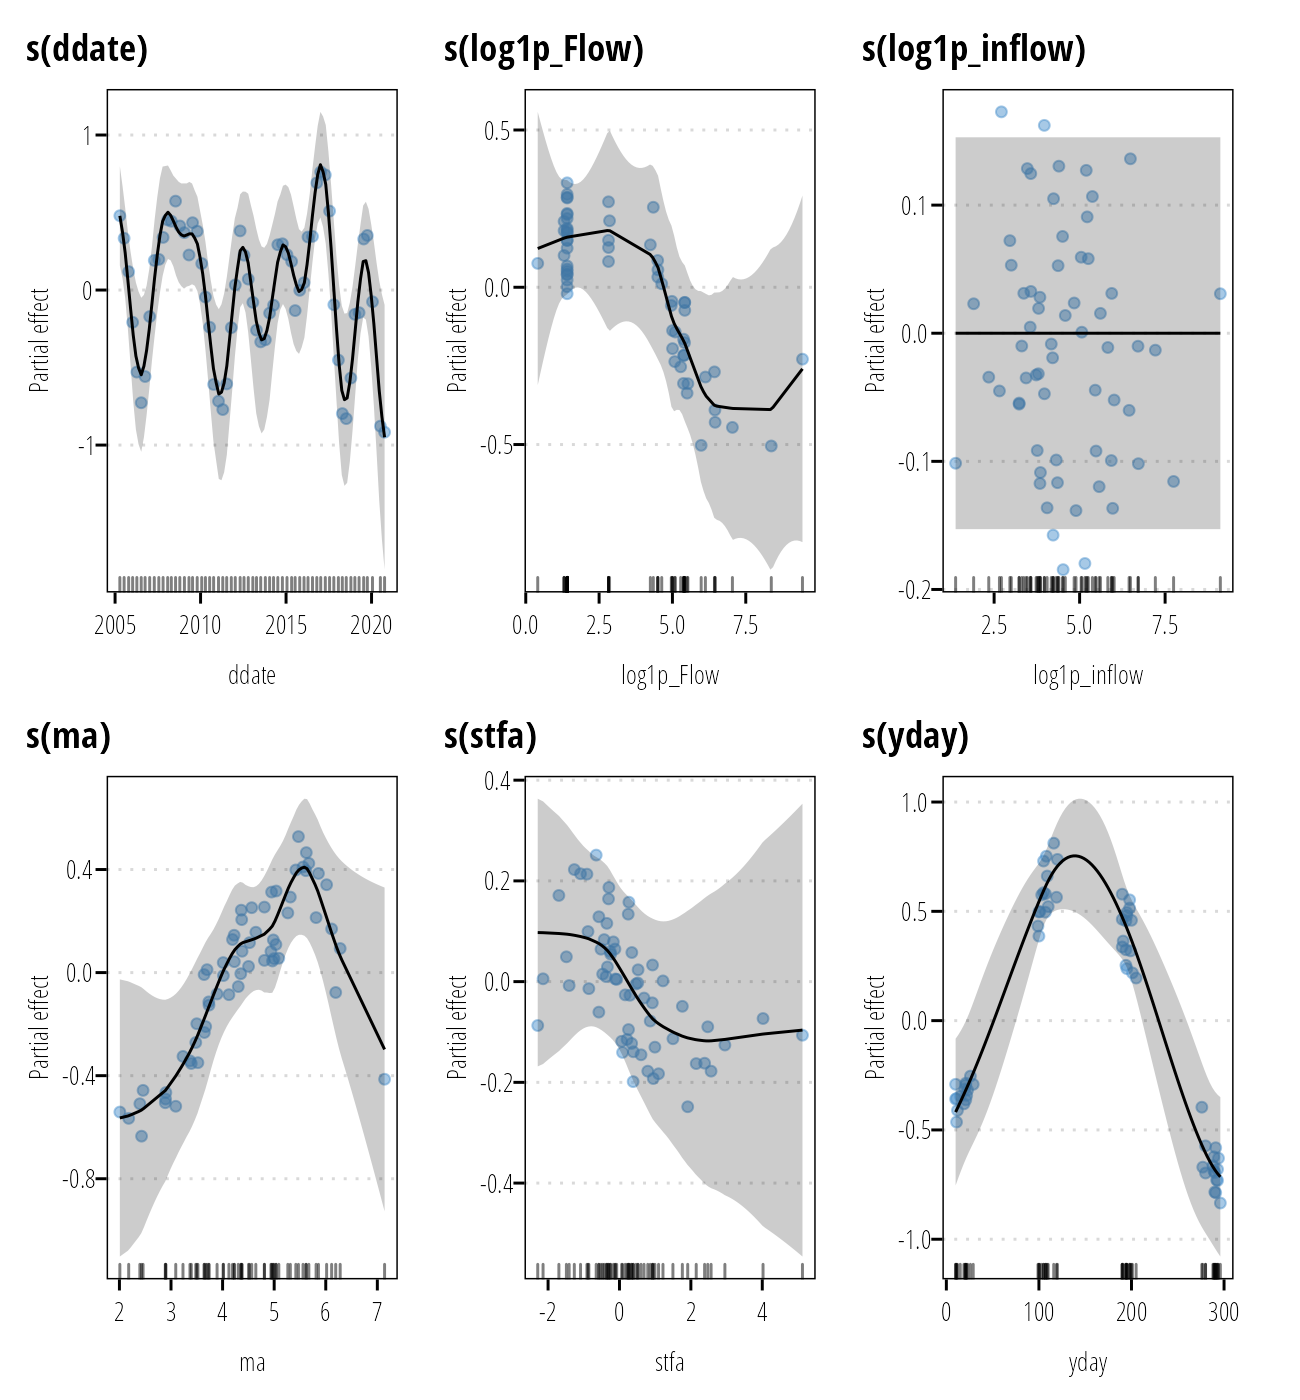
\includegraphics{model_assessment_files/figure-pdf/unnamed-chunk-65-1.png}

}

\caption{Partial effects of covariates in NO\textsubscript{3}-N model
below Palmetto Bend Dam.}

\end{figure}

\begin{figure}[h]

{\centering 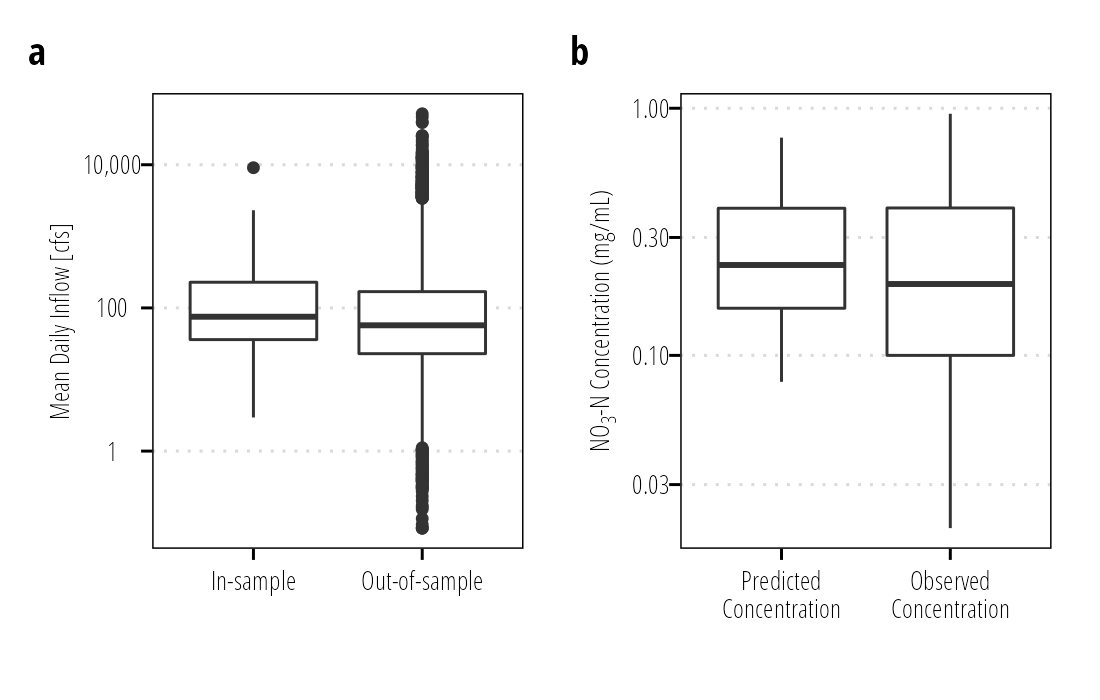
\includegraphics{model_assessment_files/figure-pdf/unnamed-chunk-66-1.png}

}

\caption{Comparisons of (a) in-sample and out-of-sample mean daily
inflows and (b) predicted daily concentration (for both sampled and
non-sampled days) and measured daily concentration.}

\end{figure}

\begin{figure}[h]

{\centering 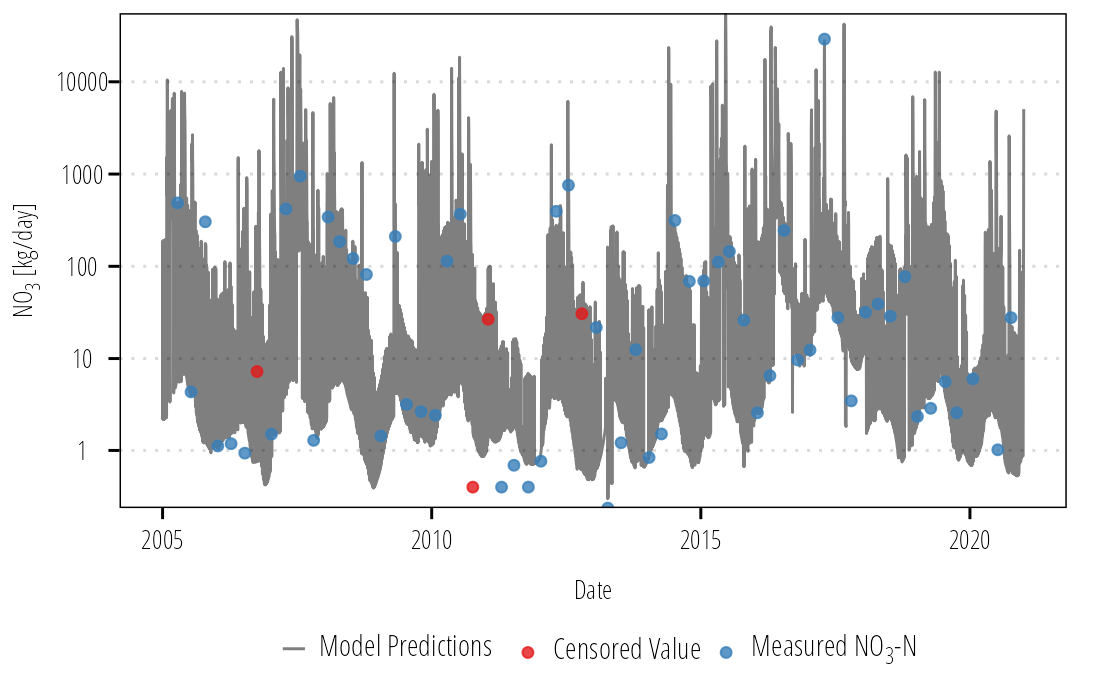
\includegraphics{model_assessment_files/figure-pdf/unnamed-chunk-67-1.png}

}

\caption{Time series plot of NO\textsubscript{3} model predictions and
observed values below Palmetto Bend Dam.}

\end{figure}

\clearpage

\hypertarget{tp-5}{%
\subsubsection{TP}\label{tp-5}}

\begin{widestuff}

\caption{TP GAM summary - Navidad River at Palmetto Bend Dam.}
\centering
\begin{tabular}[t]{llllllrll}
\toprule
Component & Term & Estimate & Std.Error & t-value & edf & ref.df & F-value & p-value\textsuperscript{1}\\
\midrule
A. parametric coefficients & (Intercept) & -1.624 & 0.037 & -44.377 &  &  &  & 0.000 ***\\
\cmidrule{1-9}
 & s(ddate) &  &  &  & 3.214 & 8 & 1.862 & 0.001 ***\\

 & s(yday) &  &  &  & 1.309 & 8 & 0.374 & 0.088 +\\

 & s(log1p(Inflow)) &  &  &  & 0.003 & 9 & 0.000 & 0.360\\

 & s(log1p(Flow)) &  &  &  & 1.104 & 4 & 0.561 & 0.098 +\\

 & s(stfa) &  &  &  & 0.000 & 5 & 0.000 & 0.470\\

\multirow[t]{-6}{*}{\raggedright\arraybackslash B. smooth terms} & s(ma) &  &  &  & 2.262 & 5 & 1.669 & 0.006 **\\
\bottomrule
\multicolumn{9}{l}{\textsuperscript{1} Signif. codes: 0 <= '***' < 0.001 < '**' < 0.01 < '*' < 0.05 < '+' < 0.1}\\
\multicolumn{9}{l}{\textsuperscript{} Adjusted R-squared: 0.321, Deviance explained 0.388}\\
\multicolumn{9}{l}{\textsuperscript{} -REML : -99.963, Scale est: 0.00403, N: 81}\\
\end{tabular}
\end{widestuff}

\hypertarget{tbl-TPPalmettoBend-CV}{}
\begin{longtable}[]{@{}lc@{}}
\caption{\label{tbl-TPPalmettoBend-CV}Summary of goodness-of-fit metrics
for 5-fold cross-validation of TP GAM at Palmetto Bend
Dam.}\tabularnewline
\toprule()
\textbf{Goodness of Fit Metric} & \textbf{Median (IQR)} \\
\midrule()
\endfirsthead
\toprule()
\textbf{Goodness of Fit Metric} & \textbf{Median (IQR)} \\
\midrule()
\endhead
KGE & 0.877 (0.862, 0.911) \\
R\textsuperscript{2} & 0.961 (0.956, 0.975) \\
Percent Bias & -17.6 (-21.1, -12.7) \\
\bottomrule()
\end{longtable}

\clearpage

\begin{figure}[h]

{\centering 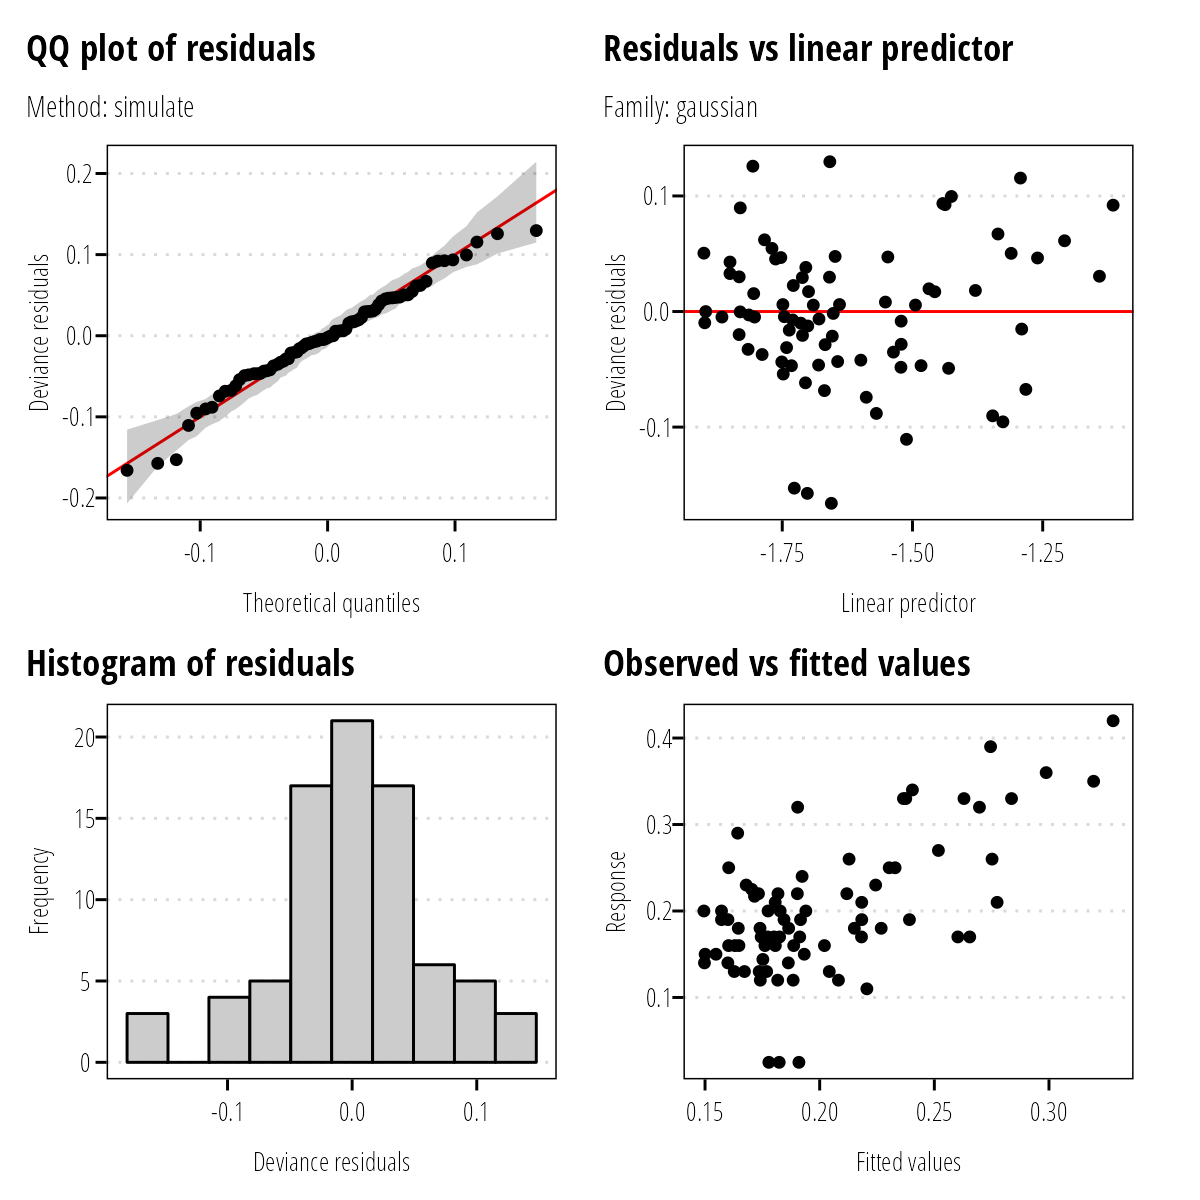
\includegraphics{model_assessment_files/figure-pdf/unnamed-chunk-70-1.png}

}

\caption{Diagnostic plot for TP model below Palmetto Bend Dam.}

\end{figure}

\begin{figure}[h]

{\centering 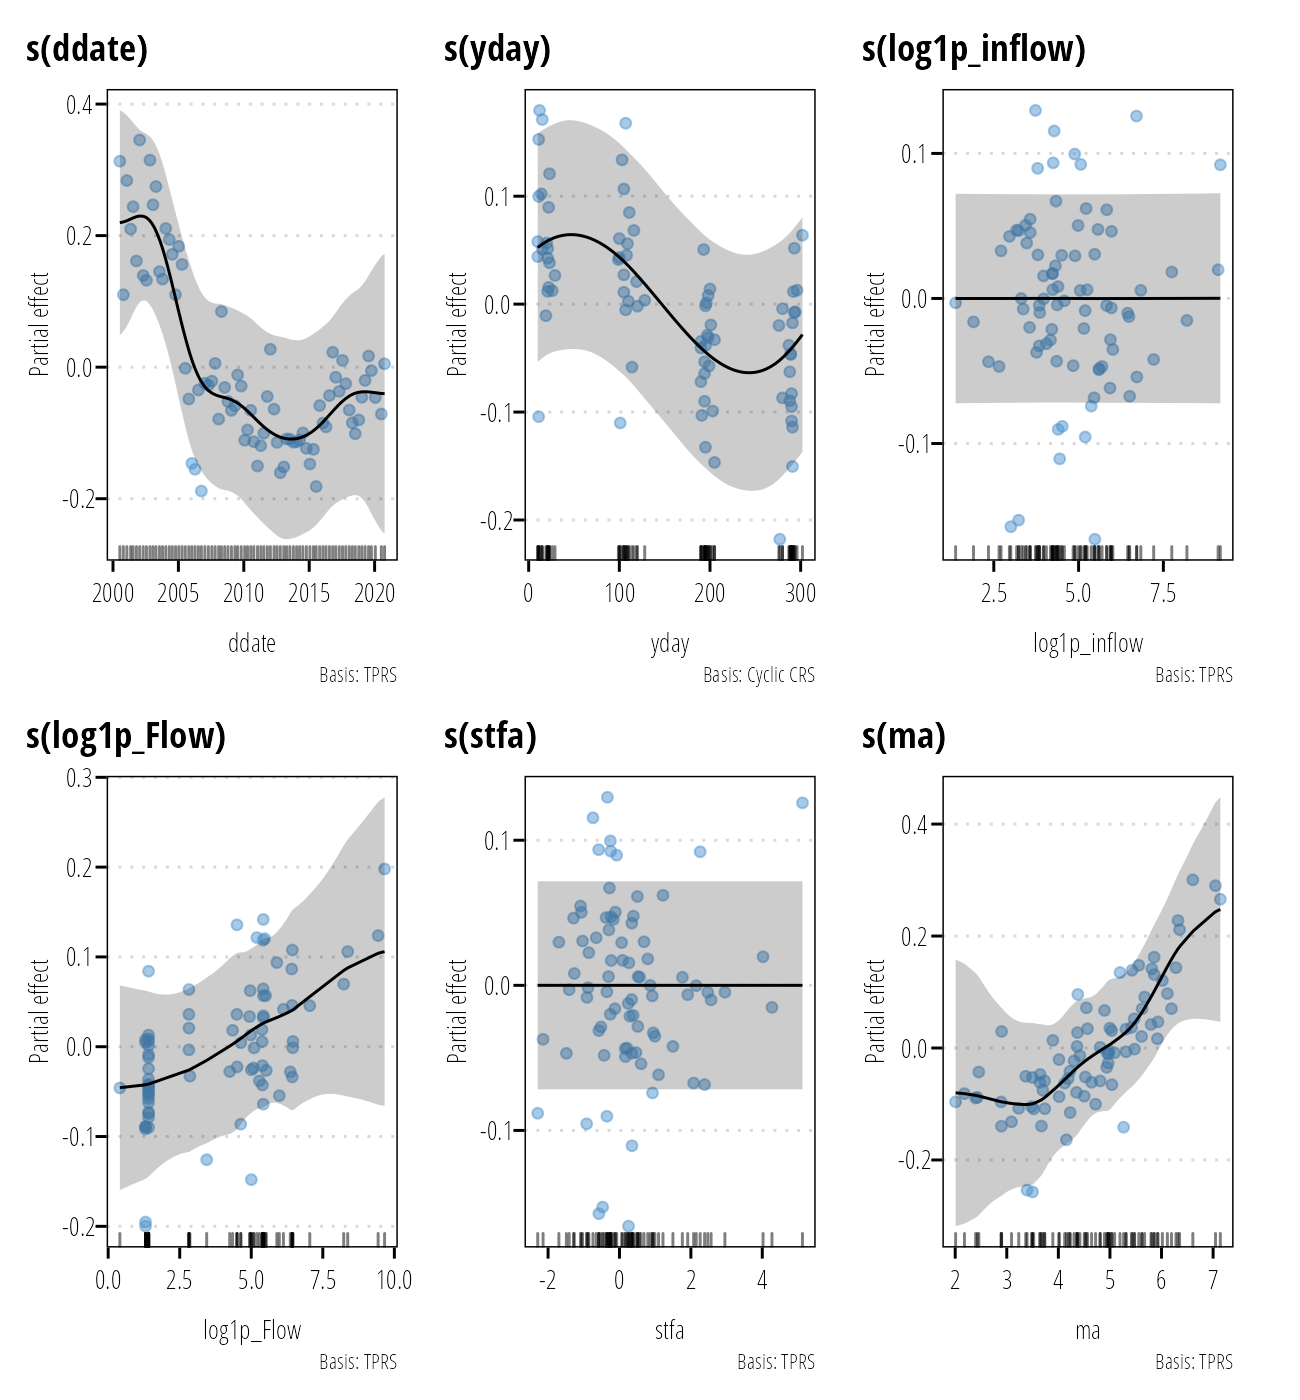
\includegraphics{model_assessment_files/figure-pdf/unnamed-chunk-71-1.png}

}

\caption{Partial effects of covariates in TP model below Palmetto Bend
Dam.}

\end{figure}

\begin{figure}[h]

{\centering 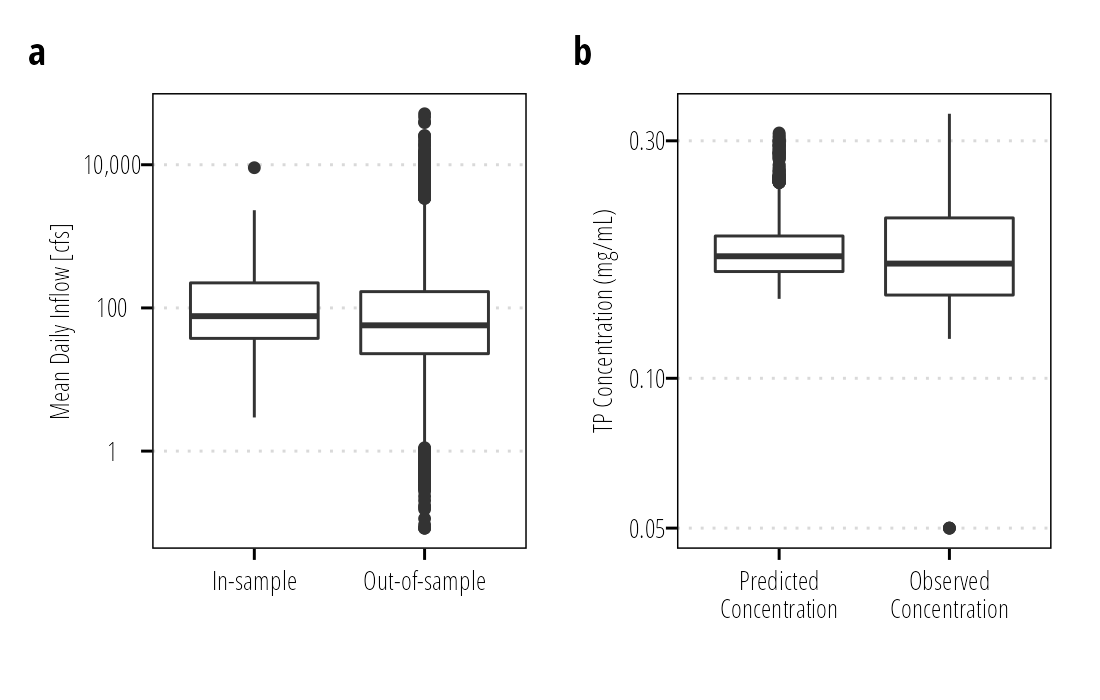
\includegraphics{model_assessment_files/figure-pdf/unnamed-chunk-72-1.png}

}

\caption{Comparisons of (a) in-sample and out-of-sample mean daily
inflows and (b) predicted daily concentration (for both sampled and
non-sampled days) and measured daily concentration.}

\end{figure}

\begin{figure}[h]

{\centering 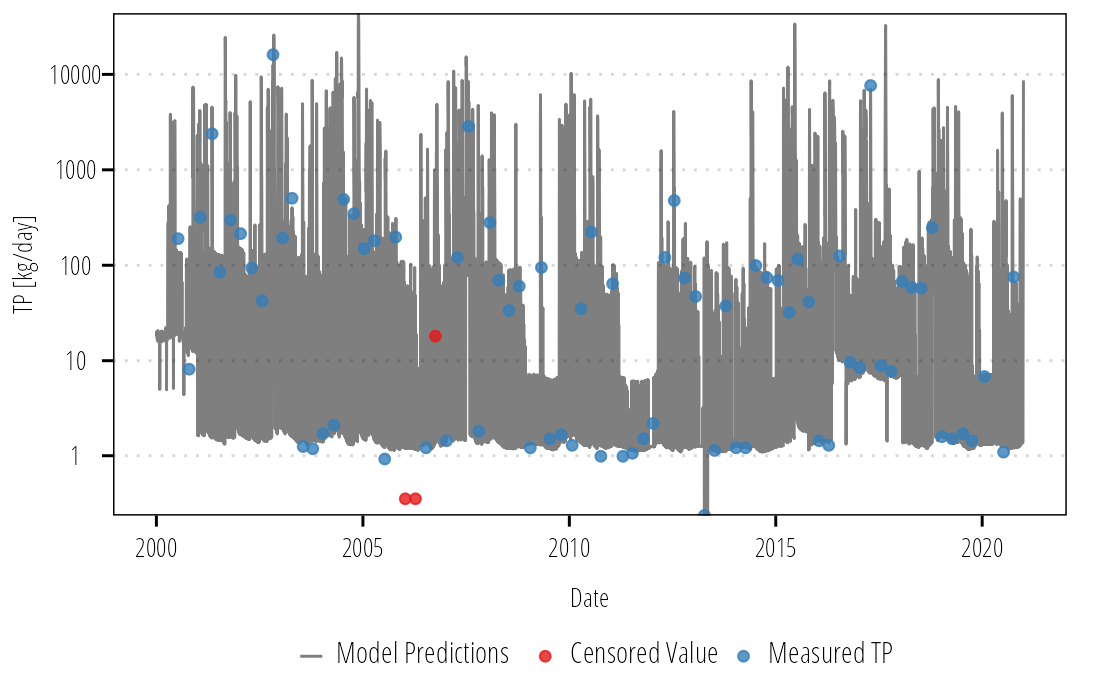
\includegraphics{model_assessment_files/figure-pdf/unnamed-chunk-73-1.png}

}

\caption{Time series plot of TP model predictions and observed values
below Palmetto Bend Dam.}

\end{figure}

\clearpage

\hypertarget{references}{%
\subsection*{References}\label{references}}
\addcontentsline{toc}{subsection}{References}

\hypertarget{refs}{}
\begin{CSLReferences}{1}{0}
\leavevmode\vadjust pre{\hypertarget{ref-beckNumericalQualitativeContrasts2017}{}}%
Beck, M.W., and Murphy, R.R. 2017. Numerical and qualitative contrasts
of two statistical models for water quality change in tidal waters.
JAWRA Journal of the American Water Resources Association 53 (1):
197--219. \url{https://doi.org/10.1111/1752-1688.12489}.

\leavevmode\vadjust pre{\hypertarget{ref-bergbuschUnexpectedShiftPhytoplankton2021}{}}%
Bergbusch, N.T., Hayes, N.M., Simpson, G.L., and Leavitt, P.R. 2021.
Unexpected shift from phytoplankton to periphyton in eutrophic streams
due to wastewater influx. Limnology and Oceanography 66 (7): 2745--61.
\url{https://doi.org/10.1002/lno.11786}.

\leavevmode\vadjust pre{\hypertarget{ref-kuhnertQuantifyingTotalSuspended2012}{}}%
Kuhnert, P.M., Henderson, B.L., Lewis, S.E., Bainbridge, Z.T.,
Wilkinson, S.N., and Brodie, J.E. 2012. Quantifying total suspended
sediment export from the Burdekin River catchment using the loads
regression estimator tool: REGRESSION ESTIMATOR TOOL FOR POLLUTANT
LOADS. Water Resources Research 48 (4).
\url{https://doi.org/10.1029/2011WR011080}.

\leavevmode\vadjust pre{\hypertarget{ref-mcdowellImplicationsLagTimes2021}{}}%
McDowell, R.W., Simpson, Z.P., Ausseil, A.G., Etheridge, Z., and Law, R.
2021. The implications of lag times between nitrate leaching losses and
riverine loads for water quality policy. Scientific Reports 11 (1):
16450. \url{https://doi.org/10.1038/s41598-021-95302-1}.

\leavevmode\vadjust pre{\hypertarget{ref-robsonPredictionSedimentParticulate2015a}{}}%
Robson, B.J., and Dourdet, V. 2015. Prediction of sediment, particulate
nutrient and dissolved nutrient concentrations in a dry tropical river
to provide input to a mechanistic coastal water quality model.
Environmental Modelling \& Software 63 (January): 97--108.
\url{https://doi.org/10.1016/j.envsoft.2014.08.009}.

\leavevmode\vadjust pre{\hypertarget{ref-zhangImprovingRiverineConstituent2017}{}}%
Zhang, Q., and Ball, W.P. 2017. Improving riverine constituent
concentration and flux estimation by accounting for antecedent discharge
conditions. Journal of Hydrology 547 (April): 387--402.
\url{https://doi.org/10.1016/j.jhydrol.2016.12.052}.

\end{CSLReferences}



\end{document}
